% !TEX encoding = utf8
% !TEX root = main.tex


%%%%%%%%%%%%%%%%%%%%%%%%%%%%%%%%%%%%%%%%%%%%%%%%%%%%  Esempio con molte opzioni
\documentclass[11pt,twoside,oldstyle,classica,greek]{toptesi}
%%%%%%%%%%%%%%%%%%%%%%%%%%%%%%%%%%%%%%%%%%%%%%%%%%%%

% Commentare la riga seguente se si è specificata l'opzione "pdfa"
\usepackage{hyperref}

\hypersetup{%
    pdfpagemode={UseOutlines},
    bookmarksopen,
    pdfstartview={FitH},
    colorlinks,
    linkcolor={blue},
    citecolor={red},
    urlcolor={blue}
  }
%
%%%%%%% Esempio di composizione di tesi di laurea con PDFLATEX <---------------- !
%
\usepackage[utf8]{inputenc}% per macchine Linux/Mac/UNIX/Windows; sarebbe meglio utf8
\usepackage[T1]{fontenc}\usepackage{lmodern}
\usepackage[italian,english]{babel}


%%%%%%%%%%%%------PACCHETTI AGGIUNTIVI------%%%%%%%%%%%%
\graphicspath{{Immagini/}} % Specifies the directory where pictures are stored
\usepackage[square, numbers, comma, sort&compress]{natbib} 
\usepackage{subfigure}
\usepackage{tikz}
\usepackage{pgfplots}
%\usepackage{indentfirst}
\usepackage{amsfonts}
\usepackage{amsmath}
\usepackage{siunitx}
%\usepackage{fancyhdr}

%\fancyhead{} % Clears all page headers and footers
%\rhead{\thepage} % Sets the right side header to show the page number
%\lhead{} % Clears the left side page header

%\pagestyle{fancy}


%
% Per scrivere testo fasullo in "latinorum"
\usepackage{lipsum}


\newcommand{\twopartdef}[4]
{
	\left\{
		\begin{array}{ll}
			#1 & \mbox{per } #2 \\
			#3 & \mbox{per } #4
		\end{array}
	\right.
}


%%%%%%% Definizioni locali
\newtheorem{teorema}{Teorema}% Standard LaTeX


\begin{document}
\interlinea{1.7}
\ateneo{Universit\`a degli Studi di Genova}
%
%%%%%%%%%%%%%%%%%%%%%
%

%
\FacoltaDi{Scuola Politecnica}

\titolo{Estrazione di \emph{feature} per classificazione di immagini telerilevate ad alta risoluzione mediante istogrammi di gradienti orientati}% per la laurea quinquennale e il dottorato
\sottotitolo{Feature extraction for high resolution remote sensing image classification using histograms of oriented gradients}% per la laurea quinquennale e il dottorato
%

\TesiDiLaurea{Tesi di Laurea Triennale}
%%%%%%% Corso degli studi
\corsodilaurea{Ingegneria Elettronica e Tecnologie dell'Informazione}% per la laurea


%%%%%%% Per inserire la matricola rientrato sotto il nome di ogni candidato.
%\renewcommand*\IDN{\\\quad matricola: }
%
\candidata{Margherita \textsc{Piccini}}% per tutti i percorsi
\secondocandidato{Simone \textsc{Rossi}}% per la laurea magistrale solamente
\terzocandidato{Eugenio \textsc{Zuccarelli}}


\relatore{Prof.\ Gabriele Moser}% per la laurea e/o il dottorato
\secondorelatore{Dott. Vladimir Krylov}% per la laurea magistrale


%%%%%%% Seduta dell'esame
%\sedutadilaurea{Agosto 1615}% per la laurea quinquennale; oppure:
%\sedutadilaurea{\textsc{Anno~accademico} 2014-2015}% per la laurea magistrale
%\esamedidottorato{Novembre 1610}% per il dottorato
\annoaccademico{2014-2015}% solo con l'opzione classica
%\annoaccademico{2006-2007}% idem
%\ciclodidottorato{XV}% solo per il dottorato

%%%%%%% Logo della sede
\logosede[4cm]{logo}% questo e' ovviamente facoltativo, ma e' richiesto per
% il dottorato al PoliTO; in questo caso si usa il "logopolito", il nome senza
% estensione del file che contiene in forma grafica il logo.
%
%%%%%%% Per cambiare l'offset per la rilegatura; meno offset c'e', meglio e'
%\setbindingcorrection{3mm}

\iflanguage{english}{%
	\sommario{Abstract}}


\frontespizio

%\sommario

\input{Frontmatter/Citazione}
\input{Frontmatter/Sommario}
\input{Frontmatter/Summary}

\input{Frontmatter/Ringraziamenti}


\tablespagetrue\figurespagetrue % normalmente questa riga non serve ed e' commentata

\indici


\mainmatter

% !TEX encoding = utf8
% !TEX root = ../main.tex


\chapter*{Introduzione}
\addcontentsline{toc}{chapter}{Introduzione}
\label{Introduzione}

Gli ultimi decenni hanno visto un crescente sviluppo di tecniche di telerilevamento orientate all'osservazione della Terra (\emph{Earth Observation} - EO), che permettono, oggigiorno, di avere un ampia disponibilità di immagini digitali, acquisite tramite sensori montati a bordo di satelliti o aviotrasportati.
Un ruolo chiave in tale ambito è stato giocato dal rapido aumento di missioni spaziali, volte alla messa in orbita di satelliti dotati di sensori con diverse caratteristiche, quali sensori ottici ad alta o altissima risoluzione spaziale e sensori ottici iperspettrali, capaci di fornire informazioni cartografiche e topografiche di grande dettaglio. 
Il dato satellitare, grazie alla multitemporalità e multispettralità delle sue osservazioni, rende possibile un monitoraggio ripetitivo di vaste aree geografiche, permettendo l'analisi di porzioni di suolo a scala globale, regionale e locale.\\
Data l'alta disponibilità di tali immagini ad alta risoluzione (\emph{Very High Resolution} - VHR), si è visto un crescente interesse per le procedure automatiche di classificazione, che permettono di classificare vaste porzioni di superficie terrestre in tempi sempre più brevi, risultando di estrema utilità a molteplici applicazioni di carattere ambientale,quali sviluppo urbano, riqualificazione di aree urbane inutilizzate, mappatura agricola, salvaguardia ambientale e gestione delle risorse naturali.\\
L'incremento della risoluzione spaziale nelle immagini telerilevate VHR ha introdotto, però, nuove problematiche nella classificazione. Se per risoluzioni basse o grossolane (ad esempio, intorno a $30/50$ metri) si può sovente evitare di tenere in considerazione l'informazione contestuale, ed accuratezze accettabili sono spesso ottenibili operando con i soli canali spettrali, per alte risoluzioni ($2-5$ metri) dettagli spaziali molto più precisi risultano apprezzabili nell'immagine ed una modellazione opportuna dell'informazione spaziale diventa necessario per discriminare accuratamente classi tematiche di interesse.
L'alta correlazione fra pixel adiacenti che sussiste a risoluzione così elevata ha portato allo studio di diversi metodi per tenere in considerazione, in fase di classificazione, la distribuzione spaziale delle intensità pixel.\\
Le due filosofie che sono nate come risposta a questo problema hanno visto coinvolti, da una parte, classificatori non contestuali affiancati a metodi di estrazione di \emph{feature} contestuali e, dall'altra, l'uso di metodi di classificazione contestuali, che esplicitamente incorporano l'informazione circa il contesto spaziale di ogni singolo pixel.\\
Tra i due, l'approccio che si è deciso di seguire in questa tesi è stato il primo: l'uso di una \emph{Support Vector Machine} (SVM), come classificatore non contestuale, affiancato all'algoritmo di \emph{histogram of oriented gradient} (HOG), per estrazione di \emph{feature}.
Con questa tesi, infatti, si desidera esplorare l'uso dell'algoritmo HOG di \emph{human detection}, testando l'applicabilità di questo approccio al contesto della classificazione di immagini di aree urbane multispettrali ad alta risoluzione. L'intento delle \emph{feature} HOG è quello di descrivere il comportamento locale del gradiente di un'immagine, cercando di enfatizzare, per quanto possibile, strutture geometriche ben definite; ciò è giustificato dal fatto che, intuitivamente, un oggetto possa essere identificato grazie al proprio contorno.\\
Il classificatore SVM è stato scelto in seguito alle sue proprietà di robustezza, al numero di \emph{feature} ed alla sua accuratezza in numerose applicazioni.\\

Questo tesi è organizzata nel seguente modo: nel Capitolo \ref{cap:telerilevamento} viene introdotto il contesto del telerilevamento, con accenni alle tipologie di sensori utilizzabili, ai tipi di classificatori e allo stato dell'arte delle varie strategie per l'estrazione di informazioni spaziali a fini di classificazione; nel Capitolo \ref{cap:hog}, invece, si è presentata un'analisi dettagliata dell'algoritmo di estrazione di \emph{feature} HOG introdotto da Dalal e Triggs \citep{Art_HOGHuman} con particolare riferimento alle modifiche da noi apportate necessarie per l'uso di questo approccio al contesto del telerilevamento di aree urbane. Il Capitolo \ref{cap:svm} propone la trattazione matematica della teoria alla base del classificatore SVM.
Nel Capitolo \ref{cap:risultati} si procede con una analisi dei risultati ottenuti con l'implementazione dell'algoritmo HOG e della SVM, valutandone la potenzialità, i punti di forza e debolezza e le situazioni nelle quali è vantaggioso o no utilizzarli, basandoci sugli indici di accuratezza introdotti nel Capitolo \ref{cap:prestazioni} e su sperimentazione condotta con tre \emph{dataset} reali particolarmente complessi.





%Gli ultimi decenni hanno visto un crescente sviluppo di tecniche di telerilevamento orientate all'osservazione della Terra (\emph{Earth Observation} - EO), che permettono, oggigiorno, di avere un ampia disponibilità di immagini digitali, acquisite tramite sensori montati a bordo di satelliti o aviotrasportati.
%Un ruolo chiave in tale ambito è stato giocato dal rapido aumento di missioni spaziali, volte alla messa in orbita di satelliti dotati di sensori con eccellenti caratteristiche, quali sensori ottici ad altissima risoluzione spaziale e sensori ottici iperspettrali, capaci di fornire informazioni cartografiche e topografiche di grande dettaglio. 
%Il dato satellitare, grazie alla multitemporalità e multispettralità delle sue riprese, rende possibile un monitoraggio repentino di vaste aree geografiche, permettendo l'analisi di porzioni di suolo a scala globale, regionale e locale.\\
%Data l'alta disponibilità di tali immagini ad alta risoluzione (\emph{Very High Resolution Image} - VHRI), si è visto un crescente interesse per le procedure automatiche di classificazione, che permettono di classificare vaste porzioni di superficie terrestre in tempi sempre più brevi, risultando di estrema utilità a molteplici applicazioni di carattere ambientale, quali studi della composizione del suolo, sviluppo urbano, riqualificazione di aree urbane inutilizzate, salvaguardia ambientale e gestione delle risorse naturali.\\
%L'incremento della risoluzione spaziale nelle immagini VHR ha introdotto, però, nuove problematiche nella classificazione. Se per risoluzioni basse o grossolane (approssimativamente $30/50$ metri) si può evitare di tenere in considerazione l'informazione contestuale, dal momento che pixel vicini hanno alta probabilità di condividere la stessa etichetta di classe, per alte risoluzioni ($5/2.5$ metri) questa approssimazione non si può più fare.  MOSERMOSER
%L'alta correlazione che sussiste a risoluzione così elevata ha portato allo studio di diversi metodi per tenere in considerazione, in fase di classificazione, la distribuzione spaziale dei pixel.\\
%Le due filosofie che sono nate come risposta a questo problema hanno visto coinvolti, da una parte, classificatori non contestuali affiancati a metodi di estrazione delle \emph{feature} aggiuntive e, dall'altra, l'uso di metodi di classificazione contestuali, che esplicitamente incorporano l'informazione circa il contesto spaziale di ogni singolo pixel.\\
%Tra i due, il metodo che si è deciso di seguire è stato il primo: l'uso di una SVM, come classificatore non contestuale, affiancato all'algoritmo di HOG, per estrazione di \emph{feature}.
%Con questa tesi, infatti, analizzare e descrivere l'implementazione dell'algoritmo HOG di \emph{human detection}, esplorando l'applicabilità di questo approccio al contesto della classificazione di immagini di aree urbane multispettrali ad alta risoluzione. L'intento delle \emph{feature} HOG è quello di descrivere il comportamento locale del gradiente di un'immagine, cercando di enfatizzare, per quanto possibile, strutture geometriche ben definite; ciò è giustificato dal fatto che, intuitivamente, un oggetto può essere identificato grazie al contorno.\\
%
%Questo documento è costituito nel seguente modo: nel Capitolo \ref{cap:telerilevamento} viene introdotto il problema del telerilevamento, con accenni alle tipologie di sensori utilizzabili, ai tipi di classificatori e allo stato dell'arte delle varie strategie per l'estrazione di informazioni aggiuntive per il miglioramento della classificazione; nel Capitolo \ref{cap:hog}, invece, è presente un'analisi dettagliata dell'algoritmo di \emph{detection} introdotto da Dalal e Triggs \citep{Art_HOGHuman} con particolare riferimento alle modifiche da noi apportate necessarie per l'uso di questo approccio al contesto del telerilevamento di aree urbane. Il Capitolo \ref{cap:svm} propone la trattazione matematica della teoria alla base del classificatore SVM, successivamente utilizzato per la fase di implementazione e test. 
%Nel Capitolo \ref{cap:risultati} si procede con una analisi puntuale e precisa dei risultati ottenuti con l'implementazione dell'algoritmo HOG e della SVM, valutandone la potenzialità, i punti di forza e debolezza e le situazioni nelle quali è vantaggioso o no utilizzarlo, basandoci sugli indici di accuratezza introdotti nel Capitolo \ref{cap:prestazioni}.

%La disponibilità di immagini satellitari per l'osservazione della Terra offre l'opportunità di avere immagini spazialmente e temporalmente uniformemente distribuite, di porzioni di superficie terrestre su diversa scala.\\
%Sensori passivi aviotrasportati acquisiscono immagini multispettrali con diversa risoluzione spettrale, in cui a ogni canale è associata una immagine in scala di grigio corrispondente ad un limitato intervallo di lunghezze d'onda dello spettro elettromagnetico. 
%Negli anni è aumentata la richiesta di disponibilità di mappe tematiche che definiscano la categoria a cui differenti porzioni di suolo appartengono.\\
%La costruzione automatizzata di queste carte è possibile grazie all'uso di tecniche di classificazione supervisionata di immagini.
%In quest'ottica, classificare immagini multispettrali con un così ampio numero di classi da distinguere è una sfida.\\

%MOSER STAR\\
%Negli ultimi decenni la tecnologia del telerilevamento ha acquisito un interesse crescente dal punto di vista del monitoraggio e della gestione ambientale, grazie alla copertura geografica ripetitiva che essa fornisce sul territorio. In seguito al numero crescente di missioni spaziali dedicate alla messa in orbita di satelliti per l'Osservazione della Terra ed alla relativa disponibilità di immagini del territorio, il telerilevamento presenta infatti ampie potenzialità per applicazioni ambientali su scala globale, regionale e locale.  
%MOSER END\\
%
%Per queste ragioni, si è visto un crescente interesse per le procedure automatiche di classificazione di immagini digitali acquisite tramite sensori, montati a bordo di satelliti o aviotrasportati. L'ampia disponibilità di tali immagini consente, oggigiorno, la classificazione di vaste porzioni di superficie terrestre in tempi sempre più brevi, risultando di estrema utilità a molteplici applicazioni di carattere ambientale, quali studi della composizione del suolo, sviluppo urbano, salvaguardia ambientale e gestione delle risorse naturali. L'alta risoluzione di queste immagini permette l'analisi di porzioni di suolo a diversa scala con un  livello di dettaglio elevato; tuttavia, la loro eterogeneità spaziale e spettrale rende complessa l'applicazione di semplici algoritmi di classificazione.\\ %, rendendo necessaria l'estrazione di parametri aggiuntivi al fine di migliorare i risultati.\\
%L'incremento della risoluzione spaziale nelle immagini VHR ha introdotto, però, nuove problematiche nella classificazione. Se per risoluzioni basse o grossolane (approssimativamente $30/50$ metri) si può evitare di tenere in considerazione l'informazione contestuale dovuta al fatto che pixel vicini hanno elevata probabilità di condividere la stessa etichetta di classe, per alte risoluzioni ($5/2.5$ metri) questa approssimazione non si può più fare. L'alta correlazione che sussiste a risoluzione così elevata ha portato allo studio di diversi metodi per tenere in considerazione, in fase di classificazione, la distribuzione spaziale dei pixel.\\
%Le due filosofie che sono nate come risposta a questo problema hanno visto coinvolti, da una parte, classificatori non contestuali affiancati a metodi di estrazione delle \emph{feature} aggiuntive e, dall'altra, l'uso di metodi di classificazione contestuali, che esplicitamente incorporano l'informazione circa il contesto spaziale di ogni singolo pixel.\\
%Tra i due, il metodo che si è deciso di seguire è stato il primo: l'uso di una SVM, come classificatore non contestuale, affiancato all'algoritmo di HOG, per estrazione di \emph{feature}. Con questa tesi, infatti, si vuole esplorare il campo di estrazione dei parametri aggiuntivi tramite l'analisi e l'implementazione dell'algoritmo HOG di \emph{human detection}, testando l'applicabilità di questo approccio al contesto della classificazione di immagini di aree urbane multispettrali ad alta risoluzione.\\
%
%
%
%Questo documento è costituito nel seguente modo: nel Capitolo \ref{cap:telerilevamento} viene introdotto il problema del telerilevamento, con accenni alle tipologie di sensori utilizzabili, ai tipi di classificatori e allo stato dell'arte delle varie strategie per l'estrazione di informazioni aggiuntive per il miglioramento della classificazione; nel Capitolo \ref{cap:hog}, invece, è presente un'analisi dettagliata dell'algoritmo di \emph{detection} introdotto da Dalal e Triggs \citep{Art_HOGHuman} con particolare riferimento alle modifiche da noi apportate necessarie per l'uso di questo approccio al contesto del telerilevamento di aree urbane. Il Capitolo \ref{cap:svm} propone la trattazione matematica della teoria alla base del classificatore SVM, successivamente utilizzato per la fase di implementazione e test. 
%Nel Capitolo \ref{cap:risultati} si procede con una analisi puntuale e precisa dei risultati ottenuti con l'implementazione dell'algoritmo HOG e della SVM, valutandone la potenzialità, i punti di forza e debolezza e le situazioni nelle quali è vantaggioso o no utilizzarlo, basandoci sugli indici di accuratezza introdotti nel Capitolo \ref{cap:prestazioni}.
% !TEX encoding = utf8
% !TEX root = ../main.tex

\chapter{Classificazione di immagini telerilevate ad alta risoluzione} 
\label{cap:telerilevamento} 

Il telerilevamento (\emph{remote sensing}) viene definito come la disciplina che permette di ricavare informazioni su oggetti posti a distanza da uno o più sensori posti non in contatto diretto con gli oggetti stessi.
Questa definizione generale comprende un vasto range di sotto-discipline atte ad estrarre informazioni, tra le quali la mappatura di dati di interesse ambientale, l'identificazione di oggetti posti sul fondale marino o fino a tecniche di \emph{human detection}.
Nel nostro caso, ci focalizzeremo in particolare nell'ambito dell'Osservazione della Terra (\emph{Earth Observation}, EO) in cui l'oggetto da analizzare sarà una porzione di suolo.
\clearpage


\section{Cenni sul Telerilevamento}


\subsection{Sensori}
Nel caso di telerilevamento al fine di \emph{EO}, i sensori sono tipicamente montati su un aereo (sensore aviotrasportato) o su un satellite (sensore satellitare), i quali, a partire dall'onda elettromagnetica incidente su di essi, generano una immagine digitale, che poi può essere elaborata da un calcolatore. 
I sensori hanno, infatti, lo scopo di acquisire parametri ambientali utili ad una successiva elaborazione delle informazioni, seguendo il procedimento rappresentato dallo schema a blocchi riportato in Figura \ref{fig:flussosistema}.

\begin{figure}[!ht]
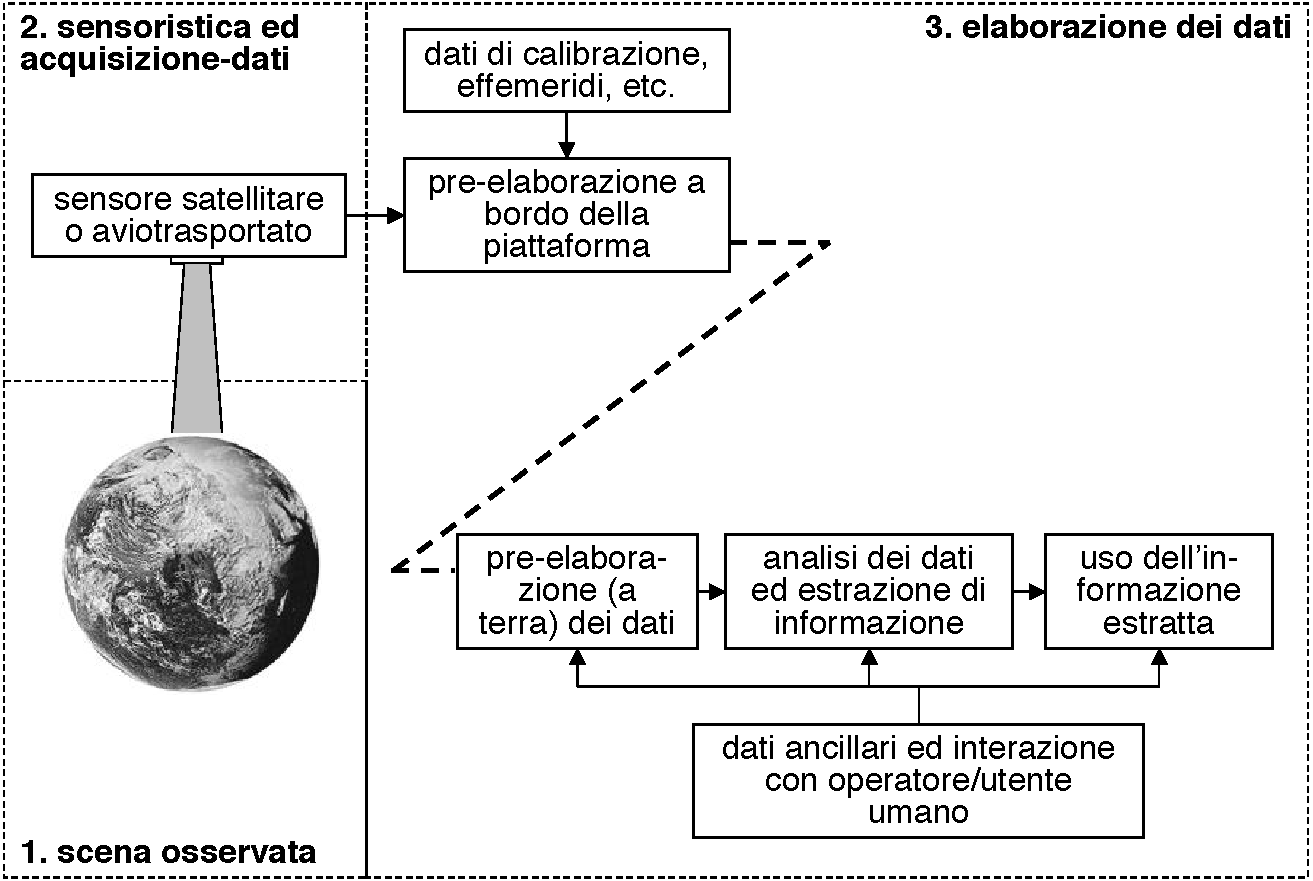
\includegraphics[width=1\textwidth]{flussosistema}
\caption{Schema a blocchi (concettuale) di un sistema di telerilevamento.}
\label{fig:flussosistema}
\end{figure}

Il procedimento generale è il seguente:
\begin{itemize}
\item innanzitutto la radiazione emessa dall'oggetto in esame (ad esempio una porzione di suolo) viene ricevuta in ingresso al sensore, per essere elaborata dal sistema;
\item il sistema di elaborazione prevede in taluni casi, una fase iniziale di pre-elaborazione dei dati a bordo della piattaforma, basata su informazioni inerenti ai sensori (ad esempio dati di calibrazione del sensore) o alla piattaforma stessa (ad esempio effemeridi);
\item successivamente, vengono effettuate operazioni di pre-elaborazione analoghe ma a terra, aventi fini quali un'ulteriore calibrazione dei dati o la rimozione di distorsioni geometriche o radiometriche dovute al movimento della piattaforma;
\item infine il sistema procede all'elaborazione vera e propria dei dati telerilevati al fine di estrarre l'informazione che viene infine fornita all'utilizzatore.
\end{itemize}


\subsection{Tipologie di sensori}

Generalmente, i sensori per telerilevamento vengono divisi in due macro-famiglie, i sensori passivi e quelli attivi.
La prima tipologia non trasmette alcun segnale, bensì, riceve unicamente la radiazione emessa dall'oggetto in esame, ovvero la radiazione elettromagnetica emessa dalla porzione di superficie, la quale può essere spontanea (tipicamente radiazione nell'intervallo dell'infrarosso vcino) oppure la radiazione riflessa o diffusa proveniente dal sole (radiazione infrarossa e/o nello spettro del visibile).
I sensori attivi, invece, trasmettono un'onda elettromagnetica nella direzione della superficie in esame e analizzano il segnale (simile ad un eco sonoro) ritrasmesso dalla porzione di suolo stessa.
Tali onde elettromagnetiche sono tipicamente segnali laser, usati da sensori \emph{LIght Detection And Ranging} (LIDAR), oppure a microonde, acquisiti tramite sensori \emph{RAdio Detection And Ranging} (RADAR).
\\

La nostra trattazione si baserà unicamente su segnali rilevati tramite sensori passivi, in particolare sensori ottici.  


\subsection{Il ruolo della risoluzione}
Un parametro di vitale importanza per un sensore orientato all' \emph{EO} è la risoluzione, con la quale si intende una risoluzione spaziale, temporale e spettrale.
La prima rappresenta il più piccolo dettaglio della superficie in esame che risulta distinguibile dopo essere stata estratta dal sensore, in particolare questo parametro è, al meglio, come la grandezza della superifcie rappresentata da un singolo pixel.
La risoluzione temporale, invece, è definita come la frequenza con cui il sensore osserva una stessa porzione di superifice. 
Essa è infatti definita come il tempo intercorso tra due passaggi del sensore sulla stessa area geografica, intervallo di tempo che può variare dal mese fino, addirittura, a poche decine di minuti.
Infine, la risoluzione spettrale viene definita come il numero di bande (o canali) misurate per ciascun pixel e dalla larghezza di banda di ogni singolo canale. Ad esempio, il sensore iperspettrale AVIRIS campiona la radiazione incidente acquisendo $224$ bande distinte, ognuna avente una larghezza pari a $9.3$ nm, rendendolo un sensore ad alta risoluzione temporale, a differenza di sensori pancromatici che elaborano solamente l'intervallo di lunghezze d'onda della radiazione visibile.


\subsection{Telerilevamento tramite sensori ottici multispettrali}
La nostra analisi si focalizzerà su sensori passivi multispettrali costituiti da sistemi di elaborazione ottica, i quali indirizzano la radiazione incidente su uno o più foto-rivelatori, che trasducono una grandezza fisica (l'intensità della radiazione elettromagnetica) in una tensione elettrica. Queste tipologie di sensori vengono trasportati da una piattaforma che viaggia ad una quota h e fa percorrere al sensore una direzione di volo (direzione \emph{in-track}), lungo la quale esso effettua uno scan lungo la direzione ortogonale (detta direzione \emph{cross-track}).
I sensori possono essere suddivisi, in base alla tecnica di scansione utilizzata, in tre famiglie:

\begin{itemize}
\item \emph{Line Scanner}, sensori che montano un solo rivelatore ottico che scandisce l'intera riga per mezzo di uno specchio oscillante;
\item \emph{Whiskbroom Scanner}, i quali possiedono un array di rivelatori orientati secondo la direzione \emph{in-track}, che scandiscono, in questo modo, più linee alla volta; 
\item \emph{Pushbroom Scanner}, contenenti un numero elevato di foto-rivelatori, lungo la direzione \emph{cross-track}, i quali permettono di scandire intere righe dell'immagine senza l'utilizzo di parti mobili.
\end{itemize}

\begin{figure}[htbp]
\centering
\subfigure[]{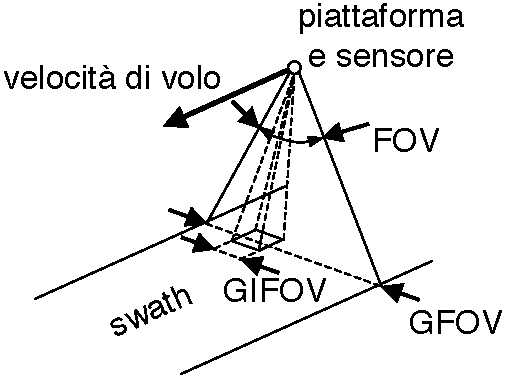
\includegraphics[width=0.3\textwidth]{linescanner}}
\qquad
\subfigure[]{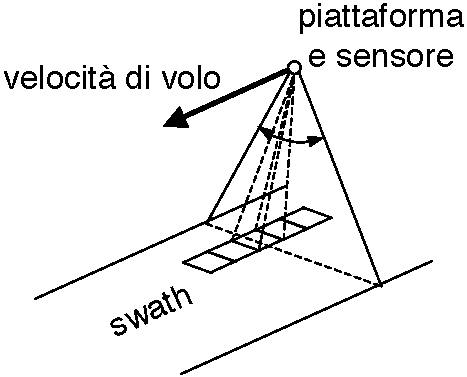
\includegraphics[width=0.3\textwidth]{whiskbroom}}
\qquad
\subfigure[]{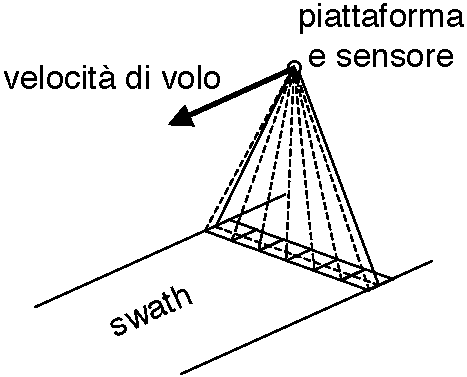
\includegraphics[width=0.3\textwidth]{pushbroom}}
\qquad
\caption{Metodi di scansione rispettivamente dei \emph{line scanner} (a), \emph{whiskbroom scanner} (b) e \emph{pushbroom scanner} (c).}
\end{figure}

Parametri chiave dei sensori ottici sono il cosiddetto \emph{Field Of View} (FOV), ovvero l'ampiezza espressa in radianti della zona di suolo osservata in direzione \emph{cross-track} e la corrispondente larghezza a terra della striscia osservata, il \emph{Ground Field Of View} (GFOV).
In modo analogo, l'estensione angolare di ogni foto-rivelatore è detta \emph{Istantaneous Field Of View} (IFOV) mentre la sua proiezione viene detta \emph{Ground Istantaneous Field Of View} (GIFOV).
Fra queste grandezze esistono delle relazioni espresse dalle seguenti equazioni:
\begin{equation}
GFOV = 2h\tan{\frac{FOV}{2}} 
\end{equation}
\begin{equation}
GIFOV = 2h\tan{\frac{IFOV}{2}}
\end{equation}
Tali sensori ottici passivi analizzano vari range di frequenze che tendenzialmente vanno dall'infrarosso termico (TIR, 8-9.5 $\si{\micro\m}$, 10-14 $\si{\micro\m}$) allo spettro del visibile (VIS, 0.4-0.7 $\si{\micro\m}$), rilevando la radianza spettrale, grandezza che permette di descrivere la distribuzione spaziale della radiazione elettromagnetica. 

\begin{table}
\caption{Principali intervalli di lunghezza d'onda significativi per il telerilevamento passivo}
\center
\begin{tabular}{cp{3cm}p{5cm}p{5cm}}
Nome							&Abbreviazione	&Lunghezza d'onda [$\mu$m]\\ \hline
Visibile							&VIS						&$0.4-0.7$\\ 
Near InfraRed				&NIR						&$0.7-1.1$\\
Short Wave InfraRed	&SWIR					&$1.1-1.35, 1.4-1.8, 2-2.5$\\
Mid Wave InfraRed		&MWIR					&$3-4, 4.5-5$\\
Thermal Infrared			&TIR						&$8-9.5, 10-14$\\
\end{tabular}
\end{table}

 \begin{figure}[!ht]
   \center
      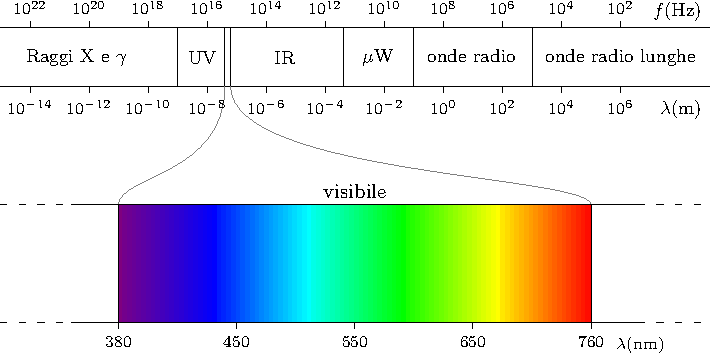
\includegraphics[width=0.8\textwidth]{spettroelettromagnetico}
    \caption{Composizione dello spettro delle onde elettromagnetiche}
    \label{fig:spettroelettromagnetico}
  \end{figure}
\clearpage




\section{Classificazione di immagini telerilevate}

\subsection{Premessa}

Si definisce classificazione di immagini telerilevate, il processo di assegnazione di una "etichetta" a ciascun pixel dell'immagine, in modo tale da renderlo appartenente ad una specifica classe, raprresentativa di una data copertura del suolo.
La classificazione è, sovente, il primo step del processo di estrazione di dati di carattere informativo da una immagine telerilevata, che vengono forniti, poi, alle successive fasi di riconoscimento (\emph{matching}) ed interpretazione. 
Queste tre fasi sono oggetto della disciplina del \emph{Pattern Recognition}, il cui obiettivo è appunto sviluppare tecniche con cui implementare, automaticamente o semi-automaticamente, i tre processi.
Oltre alla generazione di mappe tematiche tramite sistemi di telerilevamento, il \emph{pattern recognition} abbraccia vari ambiti quali l'analisi di immagini biomedicali, orientate alla robotica (\emph{Computer Vision}), o per la videosorveglianza.   

%-----------------------------------
%	SUBSECTION 2
%-----------------------------------

\subsection{Spazi di rappresentazione}

Esistono tre principali metodologie di rappresentazione dei dati, la rappresentazione nello "spazio-immagine" (\emph{Image Space}), la rappresentazione nello "spazio spettrale" (\emph{Spectral Space}) e quella nello "spazio delle feature" (\emph{Fauture Space}). La prima e più immediata consiste nel visualizzare i dati canale per canale, oppure, tramite terne RGB. La seconda tipologia consiste, invece, nel visualizzare per ciascun pixel, i livelli di grigio di ogni canale, per rappresentarli poi in un grafico. La rappresentazione nello "spazio delle \emph{feature}" si basa sull'assegnazione di assi cartesiani distinti ad ogni banda, e, così facendo, ad ogni pixel viene assopciato un vettore n-dimensionale, con n il numero di canali. Quest'ultima rappresentazione non solamente evidenzia i livelli di grigio dei pixel ma anche la distribuzione statistica nelle varie bande, rendendola generalmente piu vantaggiosa rispetto alle altre due in quanto a differenti distribuzioni nello spazio delle feature corrispondono tipicamente a differenti coperture di suolo.  

\begin{figure}[!ht]
\center
\subfigure[Rappresentazione nello spazio spettrale di un pixel di una immagine iperspettrale (220 canali) ottenuta tramite AVIRIS.]{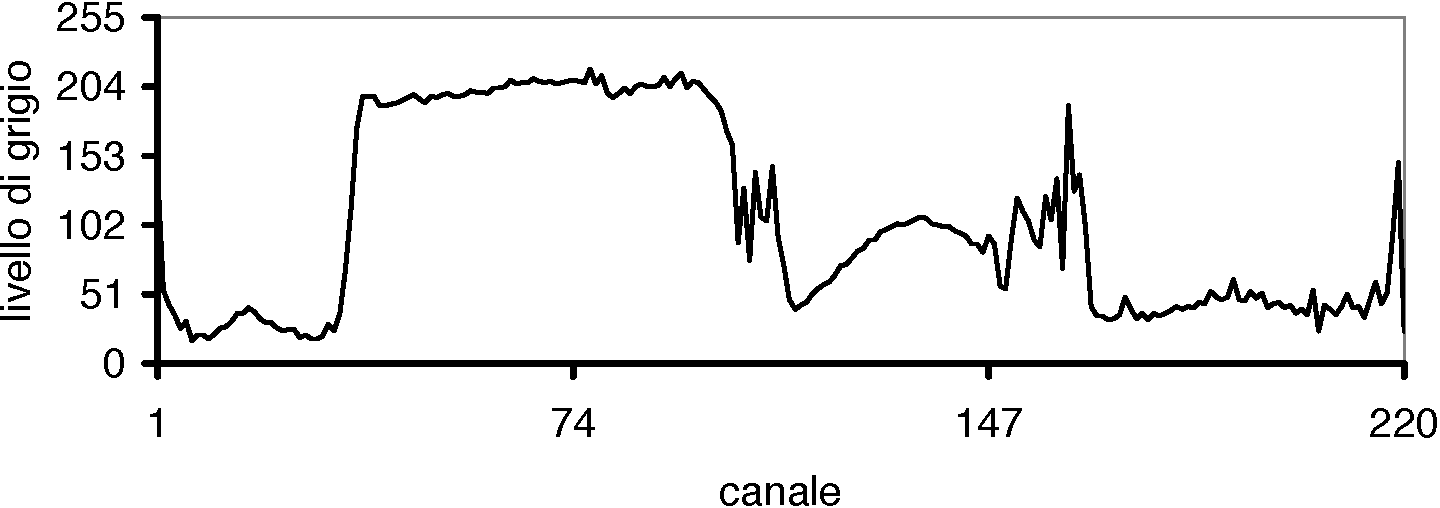
\includegraphics[width=0.4\textwidth]{indianpine_spectral}}
\hspace{3mm}
\subfigure[Rappresentazione nello spazio immagine.]{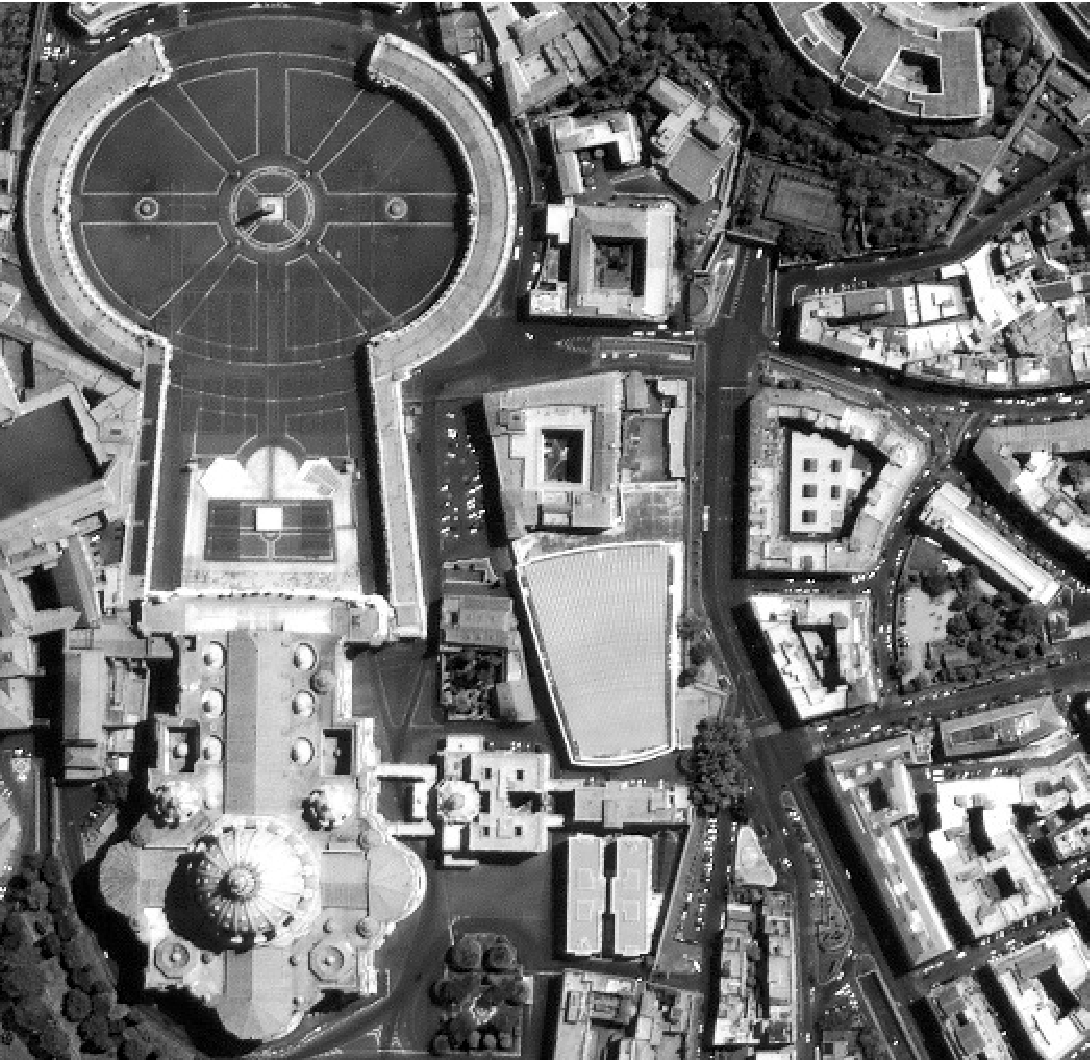
\includegraphics[width=0.4\textwidth]{vaticano}}
\\
\subfigure[Rappresentazione nello spazio delle feature.]{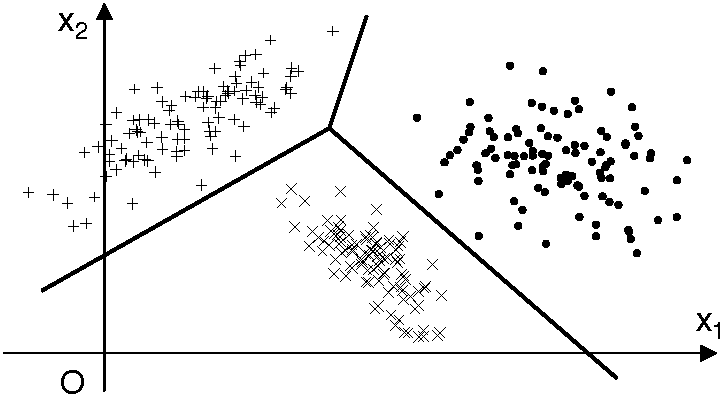
\includegraphics[width=0.5\textwidth]{featurespace}}
\caption{Esempi di rappresentazione in diversi spazi.}
\label{fig:spaziorappresentazione}
\end{figure}



%-----------------------------------
%	SUBSECTION 3
%-----------------------------------
\subsection{La classificazione nello spazio delle \emph{feature}}

A fini di classificazione, la rappresentazione nello spazio delle \emph{feature} si rivela, solitamente, la più vantaggiosa, in quanto gli andamenti spettrali di pixel appartenenti a classi distinte possono essere maggiormente separabili. In quest'ottica, classificare significa quindi partizionare lo spazio delle "feature" in opportuni sottoinsiemi, ciascuno associato ad una data classe.
\\

I classificatori possono essere divisi in due macro-famiglie, classificatori supervisionati (\emph{supervised}) e non supervisionati (\emph{unsupervised}). La prima tipologia prevede principalmente due fasi, una fase iniziale di addestramento (\emph{training}) e una di verifica (\emph{test}); nel primo step, il sistema ottimizza parametri del classificatore tramite un insieme di pixel preclassificati (\emph{training} set), fino a raggiungere una adeguata accuratezza. Successivamente, il sistema viene testato in modo analogo alla fase di training, attraverso un insieme di pixel preclassificati ma differenti rispetto a quelli coinvolti nella fase di \emph{training}.\\
Nei classificatori non supervisionati, invece, non viene utilizzato alcun \emph{training set}, solitamente perchè non sono note nè facilmente identificabili le classi coinvolte nell'applicazione in esame. 
\\

Nei capitoli a seguire la nostra attenzione sarà focalizzata sul concetto di classificazione supervisionata, che si basa, in generale, su tre assunti:
\begin{itemize}
\item si ha una conoscenza a priori esaustiva su un sottoinsieme di pixel preclassificati (\emph{training set});
\item le classi esistono in numero finito e sono note \emph{ex ante};    
\item ogni pixel è rappresentabile tramite un insieme di valori che vengono raccolti nel cosiddetto vettore delle \emph{feature} (\emph{feature vector}).
\end{itemize}


\subsubsection*{Concetti chiave e definizioni}
Data un'immagine telerilevata, a ciascun pixel $(m,n) \in \mathbb{Z}^2$ può essere associato un vettore d-dimensionale delle \emph{feature} $\textbf{x}(m,n)\in \mathbb{R}^d$, le cui componenti (le d \emph{feature}) possono essere non solamente i livelli di grigio del pixel $(m,n)$ nelle varie bande, ma anche parametri aggiuntivi come ad esempio i cosiddetti parametri di tessitura (o \emph{feature} di tessitura).\\

Le \emph{feature} di tessitura vengono estratte al fine di analizzare le differenze nella distribuzione spaziale dei livelli di grigio dei pixel, permettendo di distinguere coperture di suolo differenti. In generale, se i pixel estratti da classi differenti sono situati in zone disgiunte dello spazio delle feature, la accuratezza di classificazione è tanto maggiore quanto più sono separate le regioni. Se infatti, in una stessa regione si trovano classi distinte, esse risulteranno sovrapposte e quindi distinguerle risulterà largamente più difficoltoso.
\\

Dato un insieme $\Omega =\lbrace\omega_1,\ldots, \omega_c\rbrace$ costituito da $C$ classi distinte, note a priori, si assume che ogni oggetto o entità da analizzare sia appartenente ad una ed una sola classe (nel nostro caso ad una data copertura del suolo). A ciascun pixel è associata, quindi, anche un'etichetta di classe $y(m,n) \in \Omega$ e l'immagine $y(m,n)$ (con $m,n\in \mathbb{Z}$) è detta mappa di classificazione.
\\

Il \emph{training set} è l'insieme dei pixel di cui è nota a priori l'etichetta di classe ed è definito dall'insieme delle coppie $\left\lbrace \mathbf{x}_i,y_i \right\rbrace $, $i=1,\ldots,N$ con $N$ il numero di vettori di \emph{training} scelti. L'insieme di tali etichette rappresenta un'ulteriore immagine, detta  \emph{mappa di training}, che evidenzia alcuni pixel dell'immagine assegnati a ciascuna classe, distinguendoli dai "pixel di sfondo", cioè quei pixel per i quali l'etichetta di classe è incognita.
\\
Il processo di classificazione, come già accennato precedentemente, è diviso in due passi: \emph{learning} e \emph{prediction} (fase di addestramento e fase di predizione). Lo scopo della fase di \emph{learning} è quello di costruire un modello di classificatore, tramite la definizione di una \emph{regola di decisione} (o anche detta \emph{funzione discriminante}). \\
In termini generali, la \emph{regola di decisione} è una funzione $f:\mathbb{R}^d\rightarrow\mathbb{R}$ modellata sulla base dell'andamento statistico del \emph{training set} in modo tale che $f$ valutata per un pixel incognito restituisca una stima dell'etichetta da associargli. Le funzioni discriminanti possono essere definite con vari metodi, cui corrispondono varie tecniche di classificazione (nel Capitolo \ref{cap:svm} ne viene descritto uno dei possibili). \\
Conclusa questa fase, si procede con la classificazione vera e propria: si scandisce l'intera immagine valutando ogni pixel tramite la \emph{regola di decisione}, realizzando, in questo modo, una stima della mappa di classificazione.

\tikzstyle{block} = [rectangle, draw, %fill=blue!20, 
     text width=8em, text centered, rounded corners, minimum height=3em]
\tikzstyle{arrow} = [draw, -latex]
\tikzstyle{line} = [draw]


\begin{figure}[!ht]
\center
\begin{tikzpicture}
\node[](training) at (0,0) {$\left\lbrace \mathbf{x}_i,y_i \right\rbrace $};
\node[] at (0,.5){Training set};
\node[block] (addestramento) at (4,0) {Addestramento};
\node[](decision_rule) at (10,0) {Regola di decisione};
\node[](node1) at (7,.1){};
\node[block](prediction) at (7,-2) {Predizione};

\node[](image) at (3,-2) {$ \mathbf{X}(m,n)$};
\node[] at (3,-1.5){Immagine};

\node[]() at (11,-1.5) {Mappa di classificazione};
\node[](classmap) at (11,-2) {$Y(m,n)$};

\path[arrow] (training)--(addestramento);
\path[arrow] (addestramento) -- (decision_rule);
\path[arrow] (node1)--(prediction);
\path[arrow] (image)--(prediction);
\path[arrow] (prediction)--(classmap);
\end{tikzpicture}
    \caption{Schema funzionale di un classificatore}
    \label{fig:flowchart_classificatore}
  \end{figure}
\clearpage


\section{Il ruolo dell'informazione spaziale}

Una ulteriore distinzione che permette di differenziare tra loro le tipologie di classificatori è quella inerente al ruolo dei pixel adiacenti nella analisi della copertura al suolo. Esistono, infatti, classificatori cosiddetti non contestuali, in cui la copertura viene analizzata senza tener conto dei pixel adiacenti, risparmiando così un alto costo computazionale, ma trascurando la forte correlazione tra pixel limitrofi. Infatti, la probabilità che una regione dell'immagine sia formata da pixel tutti appartenenti alla stessa classe è molto elevata; si pensi solamente a zone boschive o fluviali. 
\\

Queste due tipologie di classificatori sono chiaramente differenti anche in base all'ambito in cui vengono applicate; mentre le tecniche di classificazione supervisionata non contestuale risultano molto efficaci e largamente consolidate per le immagini con una risoluzione piuttosto grossolana, esse mostrano forti limiti per le immagini \emph{Very High Resolution}. 
Una maggiore risoluzione spaziale comporta, infatti, una maggiore eterogeneità e una corrispondente buona definizione delle strutture geometriche quali strade e edifici, caratteristiche che rendono necessario l'utilizzo di classificatori contestuali. 
A tal fin, un ruolo chiave viene giocato principalmente da tre approcci metodologici, l'estrazione di parametri di tessitura, metodi basati su regioni e oggetti e i \emph{Markov Random Field} (MRF).


\subsection*{Estrazione dei parametri di tessitura}
L'estrazione di \emph{texture} ha come obiettivo quello di rilevare, in una determinata regione dell'immagine, strutture ripetitive nella distribuzione spaziale dei pixel quali zone urbane o boschive. 
Ciò fornisce una sorgente di dati complementare per le applicazioni in cui l'informazione relativa unicamente allo spettro dell'immagine risulta non sufficiente ai fini della classificazione. 
Le principali tecniche di estrazione di parametri di tessitura si basano sui semivariogrammi, che consistono in una statistica del secondo ordine delle intensità dei pixel, sulla morfologia matematica, sull'uso della matrice di co-occorrenza dei livelli di grigio, o su statistiche associate a confronti i istogrammi locali. Il calcolo di tali feature coinvolge tipicamente l'uso di algoritmi basati su finestre mobili.


\subsection*{Tecniche Region-based}
Gli approcci basati invece sulle regioni (\emph{region-based methods}) si basano su tecniche che puntano a suddividere le immagini in segmenti o regioni omogenee. In generale, una buona tecnica di segmentazione possiede:
\begin{itemize}
\item pixel nella stessa categoria aventi livelli di grigio simili che formano una regione connessa;
\item pixel adiacenti che sono in categorie differenti hanno valori differenti. 
\end{itemize}


\subsection*{Markov Random Field}
I \emph{Markov Random Fields}, che generalizzano il concetto di catena markoviana monodimensionale ad un sistema 2D, massimizzano l'accuratezza tramite la dipendenza che sussiste tra pixel adiacenti. 
Essi offrono, infatti, una soluzione computazionalmente efficiente per restringere la zona di interesse dall'intera immagine (elaborazione globale) ad un intorno del pixel (elaborazione locale). 
In particolare, siano $i$ e $j$ due pixel dell'immagine, si ha allora che se la funzione di probabilità $P(Y)>0$ per ogni configurazione $Y$ e se la seguente condizione è garantita per tutti i pixel i dell'immagine, si ha allora che:
\begin{equation}
P(y_i|y_j, j \neq i) = P(y_i|y_j, j\sim i)
\end{equation}   

con $i\sim j$ che indica che i pixel i e j sono vicini rispetto ad un sistema di intorni definito sul reticolo dei pixel.\\

Ciò indica che la distribuzione di probabilità delle etichette di ciascun pixel $i$, condizionata ai valori di tutti gli altri pixel dell'immagine, può essere ristretta alla distribuzione delle etichette di $i$ condizionato solamente alle etichette dei pixel adiacenti. Si può chiaramente osservare come tale definizione sia una generalizzazione dei processi markoviani monodimensionali, in cui la probabilità di transizione da uno stato ad un altro dipende unicamente dallo stato precedente.
    


% Chapter Template
%!TEX root = ..\main.tex

\chapter{Istogrammi di gradienti orientati per classificazione di immagini} % Main chapter title
\label{cap:hog}

In questo capitolo verrà presentato il metodo di estrazione di \emph{feature} tramite istogrammi di gradienti orientati (\emph{Histogram of Oriented Gradients}, HOG). Questo metodo, introdotto per la prima volta da Dalal e Triggs \citep{Art_HOGHuman}, si basa sulla valutazione di istogrammi calcolati in base a direzione e intensità dei gradienti dell'immagine in ingresso. L'idea di base è che la forma di un oggetto può essere rappresentata in modo esaustivo dalla distribuzione di modulo e fase dei gradienti locali. 
\clearpage

\section{Schema generale dell'algoritmo}
In pratica, dopo aver calcolato il gradiente dell'immagine punto per punto, essa viene divisa in piccole regioni spaziali denominate "celle". Per ogni cella viene costruito un istogramma sulla base della direzione del gradiente dei suoi pixel. Per una migliore invarianza agli effetti dovuti all'illuminazione viene effettuata una normalizzazione degli istogrammi delle celle, ottenuta sulla base di una regione spaziale di dimensione maggiore denominata "blocco". I singoli istogrammi, combinati, danno origine ai vettori delle \emph{feature} che vengono poi utilizzate da un classificatore, al fine di classificare l'immagine di partenza. Lo schema a blocchi del descrittore HOG è rappresentato in Figura \ref{fig:Schema_HOG}.
 \\

\tikzstyle{block} = [rectangle, draw, %fill=blue!20, 
     text width=6em, text centered, rounded corners, minimum height=3em]
\tikzstyle{line} = [draw, -latex]
%\tikzstyle{cloud} = [draw, ellipse,fill=red!20, node distance=3cm,
%    minimum height=2em]
 \begin{figure}[!ht]
    
\begin{tikzpicture}[node distance = 2.75cm,]
    % Place nodes
    \node [] (input_image) {\begin{footnotesize} Immagine in ingresso \end{footnotesize}};
    \node [block, above of=input_image, node distance=1.5cm] (normalizzazione_gamma_colore) {{\footnotesize Riduzione\\ rumore}};
    \node [block, right of=normalizzazione_gamma_colore] (gradiente) {\footnotesize Calcolo gradienti};
    \node [block, right of=gradiente] (pesatura_bins) {\footnotesize Costruzione \\ istogrammi};
    \node [block, right of=pesatura_bins] (normalizzazione_blocco) {\footnotesize Normalizzazione\\ contrasto};
    \node [block, right of=normalizzazione_blocco] (features) {\footnotesize Costruzione vettore delle features};
    \node [ below of=features,node distance=1.5cm] (classificatore) {\footnotesize Classificatore};

    % Draw edges
    \path [line] (input_image) -- (normalizzazione_gamma_colore);
    \path [line] (normalizzazione_gamma_colore) -- (gradiente);
    \path [line] (gradiente) -- (pesatura_bins);
    \path [line] (pesatura_bins) -- (normalizzazione_blocco);
    \path [line] (normalizzazione_blocco) -- (features);
    \path [line] (features) -- (classificatore);

\end{tikzpicture}
 \caption{Schema a blocchi del metodo HOG}
 \label{fig:Schema_HOG}
 \end{figure}

Di seguito verranno riportate in maniera dettagliata le singole fasi che lo costituiscono, evidenziando le scelte progettuali e analizzando come i diversi parametri varino la prestazione.


%	SUBSECTION 1
%-----------------------------------
%\subsection{Normalizzazione Gamma/Colore}
%L'Immagine di Ingresso all'algoritmo può essere inizialmente normalizzata attraverso una correzione di gamma al fine di uniformare le diverse rappresentazioni dei pixel dell'immagine in ingresso (scala di grigio, RGB, LAB). Questa normalizzazione ha effetti limitati per quanto riguarda la performance, che invece può essere regolata variando i parametri su dimensione di celle e blocchi. Per questo  motivo abbiamo optatato per non introdurre la correzione gamma nel nostro descrittore.

%-----------------------------------
%	SUBSECTION 2
%-----------------------------------

\section{Pulitura dal rumore}

%----------------------------------------------------------------------------------------
%	SECTION 2
%----------------------------------------------------------------------------------------
La strumentazione del sensore passivo multispettrale introduce, in generale, disturbi nella misura della radianza, dovuta ad esempio ad una variazione di riflettanza, emittanza o illuminazione solare indicati complessivamente con il termine di rumore. 
Questo può essere modellato come rumore additivo gaussiano\footnote{Come conseguenza del teorema centrale del limite, la distribuzione di probabilità di ogni pixel può essere modellata come gaussiana, visto l'elevato numero di contributi di variabili che concorrono alla definizione del pixel stesso.}.
Per limitarne gli effetti sull'immagine di ingresso, è opportuno applicare un filtraggio di pulizia dal rumore.\\

La riduzione del rumore (\emph{noise cleaning}) può essere ottunuta tramite la convoluzione con una gaussiana bidimensionale (Figura \ref{fig:Gaussiana3D}) che, essendo notoriamente un passabasso, elimina o riduce le frequenze dove il contenuto spettrale di rumore è maggiore di quello delle immagini.
Lo stesso tipo di filtraggio può essere applicato anche sulle immagini in uscita dall'algoritmo HOG.\\


La gaussiana di varianza $\sigma_{x}$ $\sigma_{y}$ è data da:
\begin{equation}
\label{eq:Gaussiana_continua}
H_{\sigma}(x,y)= \frac{1}{\sigma_{x}\cdot \sqrt{2\pi}}\cdot e^{-\frac{x^{2}}{(\sigma_{x})^{2}}}\cdot\frac{1}{\sigma_{y}\cdot \sqrt{2\pi}}\cdot e^{-\frac{y^{2}}{(\sigma_{y})^{2}}}
\end{equation}

\begin{figure}[!ht]
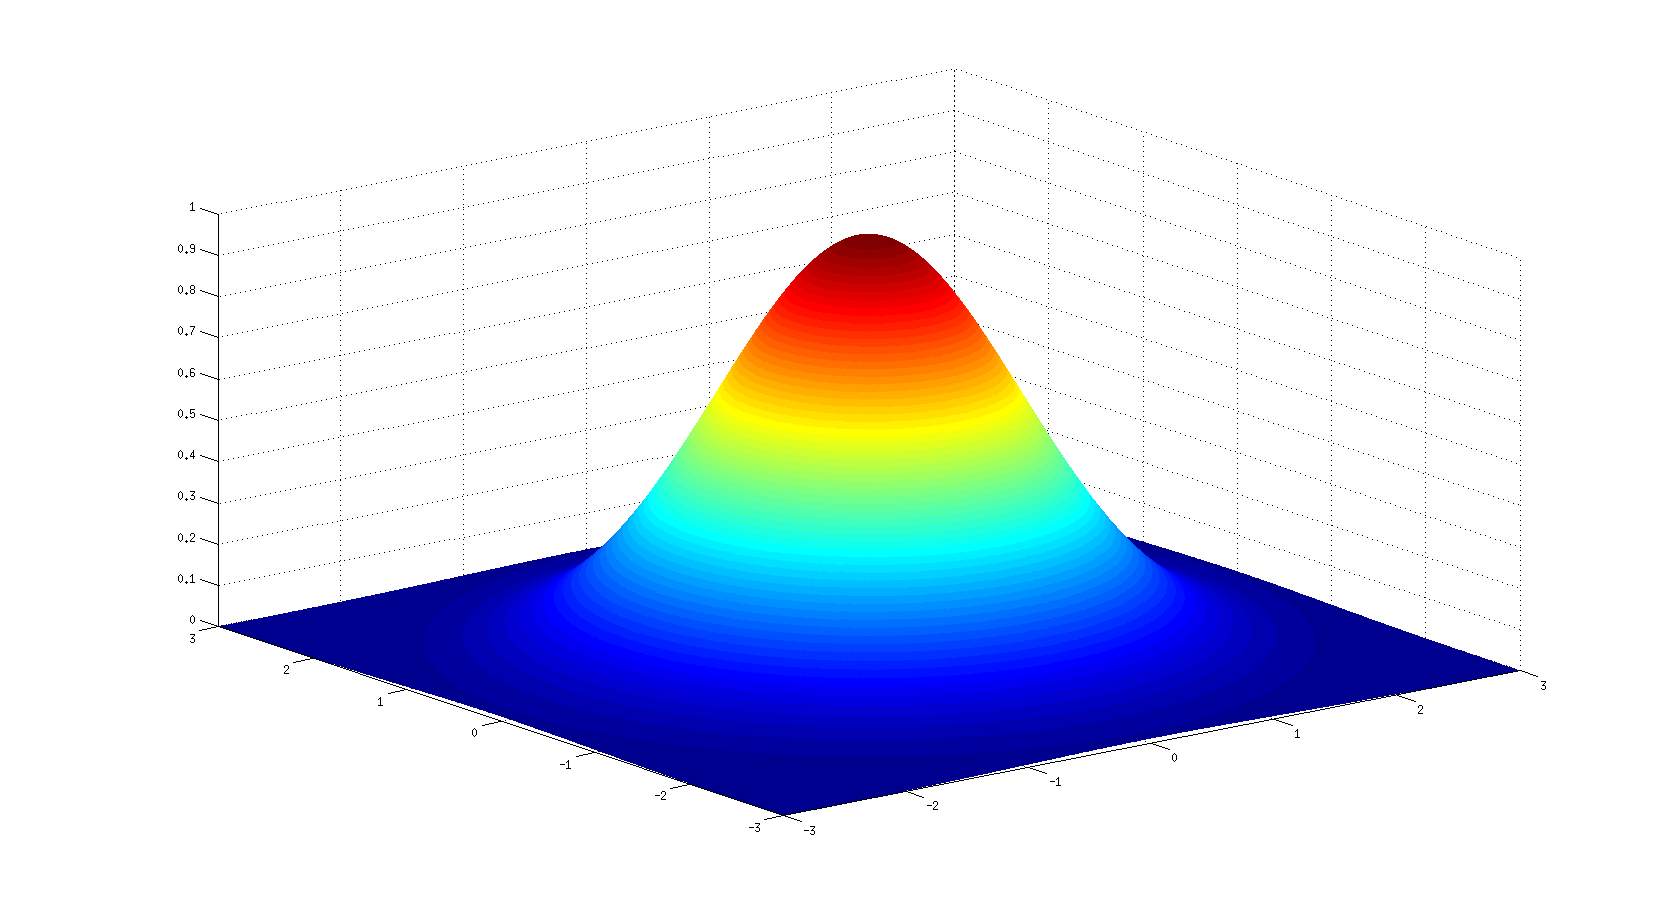
\includegraphics[width=1\textwidth]{Gaussiana3D}
\caption{Gaussiana in 3D di varianza $\sigma_{x}$ $\sigma_{y}$ e media nulla}
\label{fig:Gaussiana3D}
\end{figure}

La sua versione discreta si ottiene campionandola su una finestra quadrata di dimensioni $K \times K$ con $K> 3\cdot 2 \sqrt{\sigma}$ per rendere trascurabili gli effetti del troncamento. 
La maschera così ottenuta viene moltiplicata per $\frac{1}{c}$, dove il fattore di normalizzazione $c$ è  scelto in modo tale che: 
\begin{equation}
\label{eq:normalizzazione_gaussiana}
\sum_j\sum_k g_{jk} = 1
\end{equation} 
dove $g_{jk}$ è il generico elemento della gaussiana campionata.


\begin{figure}[!ht]
\centering
\subfigure[Immagine originale con rumore spazialmente uniforme]{
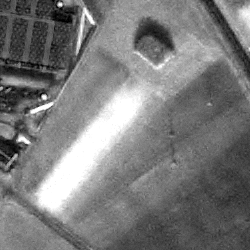
\includegraphics[scale=0.5]{immagine_non_filtrata}}
\hspace{3mm}
\subfigure[Risultato di filtraggio gaussiano]{
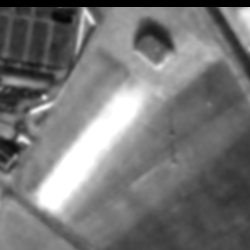
\includegraphics[scale=0.5]{immagine_filtrata}}
\caption{Riduzione del rumore nell'immagine di test tramite filtraggio gaussiano a media nulla e varianza $\sigma = 2$ pixel}.
\label{fig:immagine_rumore}
\end{figure}


\section{Calcolo dei Gradienti}
Il gradiente di un'immagine misura la variazione direzionale di intensità della stessa.
Matematicamente, il gradiente di una funzione a due variabili  associa ad ogni punto dell'immagine un vettore 2D con componenti date dalle derivate calcolate sulle direzioni orizzontali e verticali. 
Poiché la funzione intensità di un' immagine è conosciuta solo in punti discreti, si assume che le sue derivate siano calcolate su di una funzione intensità continua campionata nei punti dell'immagine.
\\

Dal punto di vista matematico, detta $F(x,y)$ una funzione continua e derivabile, il suo gradiente è dato da:
\begin{equation}
\label{eq:gradiente}
\nabla F=\frac{\partial F}{\partial x}\hat x + \frac{\partial F}{\partial y}\hat y
\end{equation}
dove:
\begin{itemize}
\item $\frac{\partial F}{\partial x}=G_{x}$ è il gradiente calcolato lungo la direzione x;
\item $\frac{\partial F}{\partial y}=G_{y}$ è il gradiente calcolato lungo la direzione y.
\end{itemize}

\begin{figure}[!ht,scale=0.8]
\centering
\subfigure[Immagine originale]{
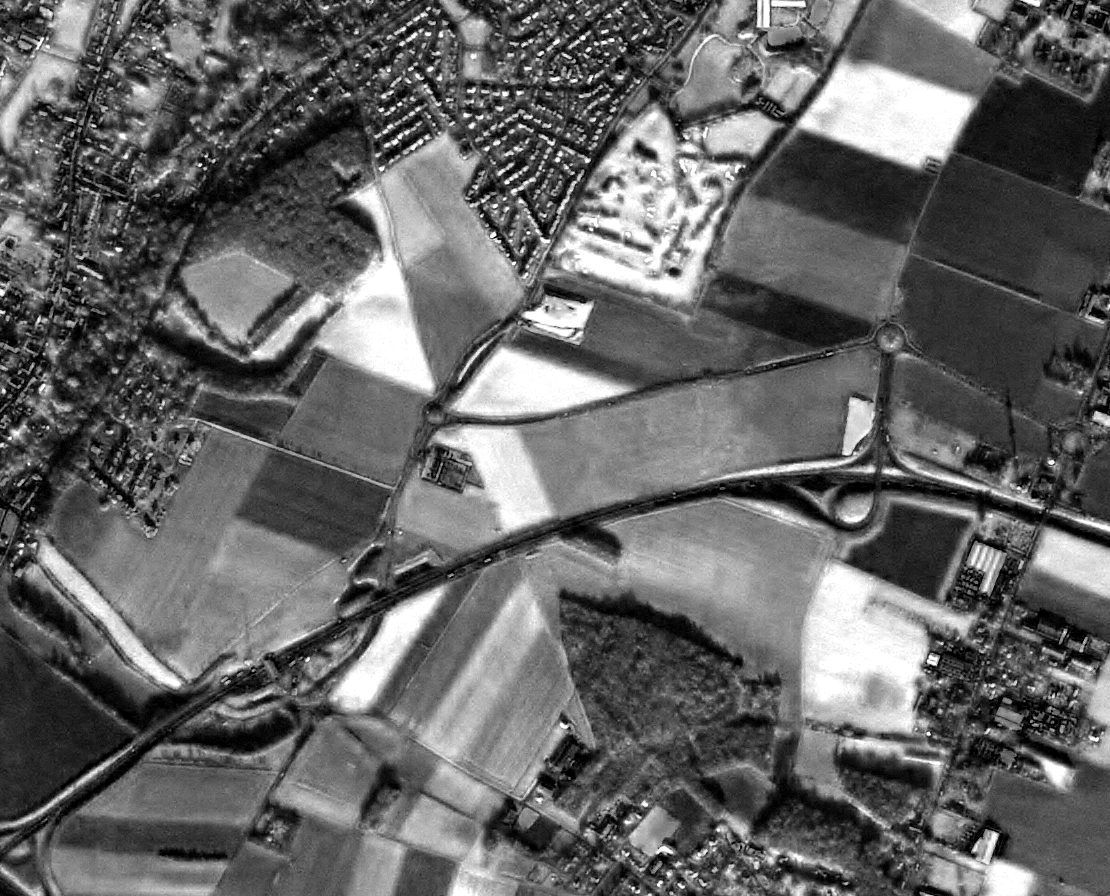
\includegraphics[scale=0.15]{immagine_originale_primagradiente}}
\\
\subfigure[Gradiente rispetto alla direzione x]{
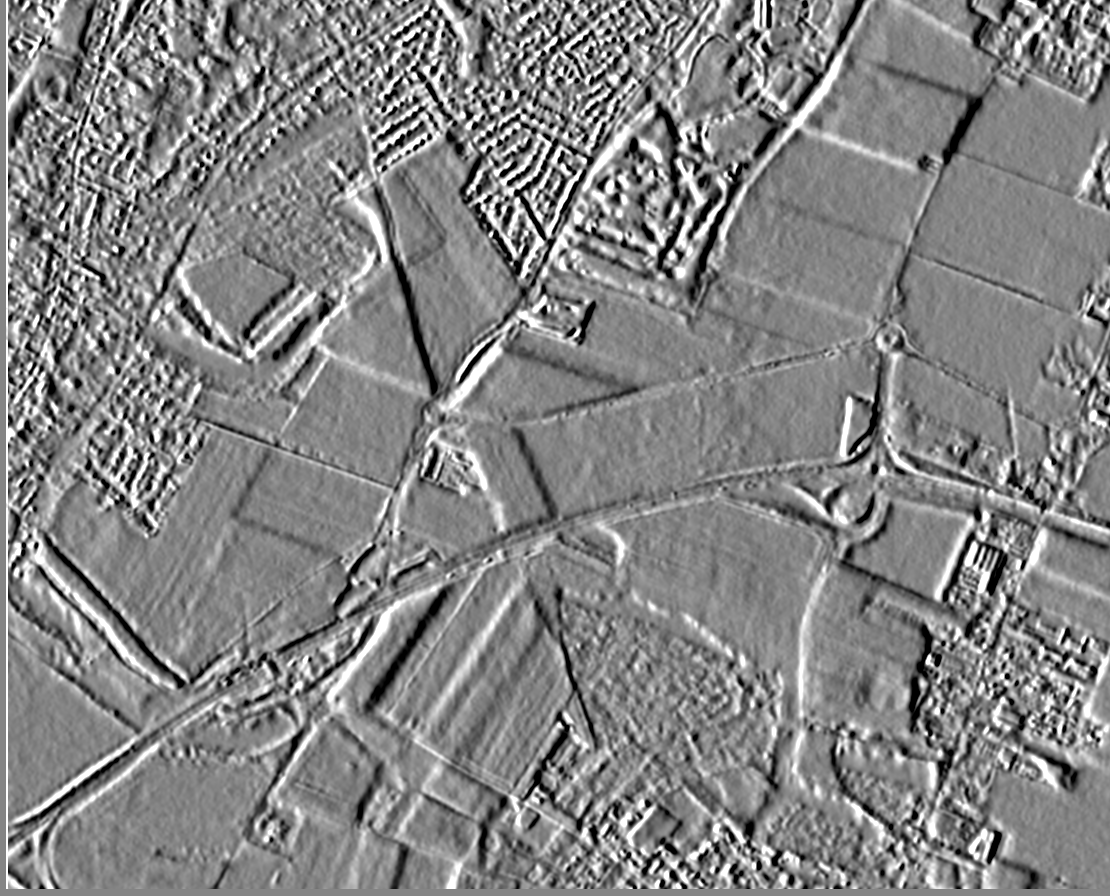
\includegraphics[scale=0.15]{Gradiente_rispetto_x}}
\hspace{3mm}
\subfigure[Gradiente rispetto alla direzione y]{
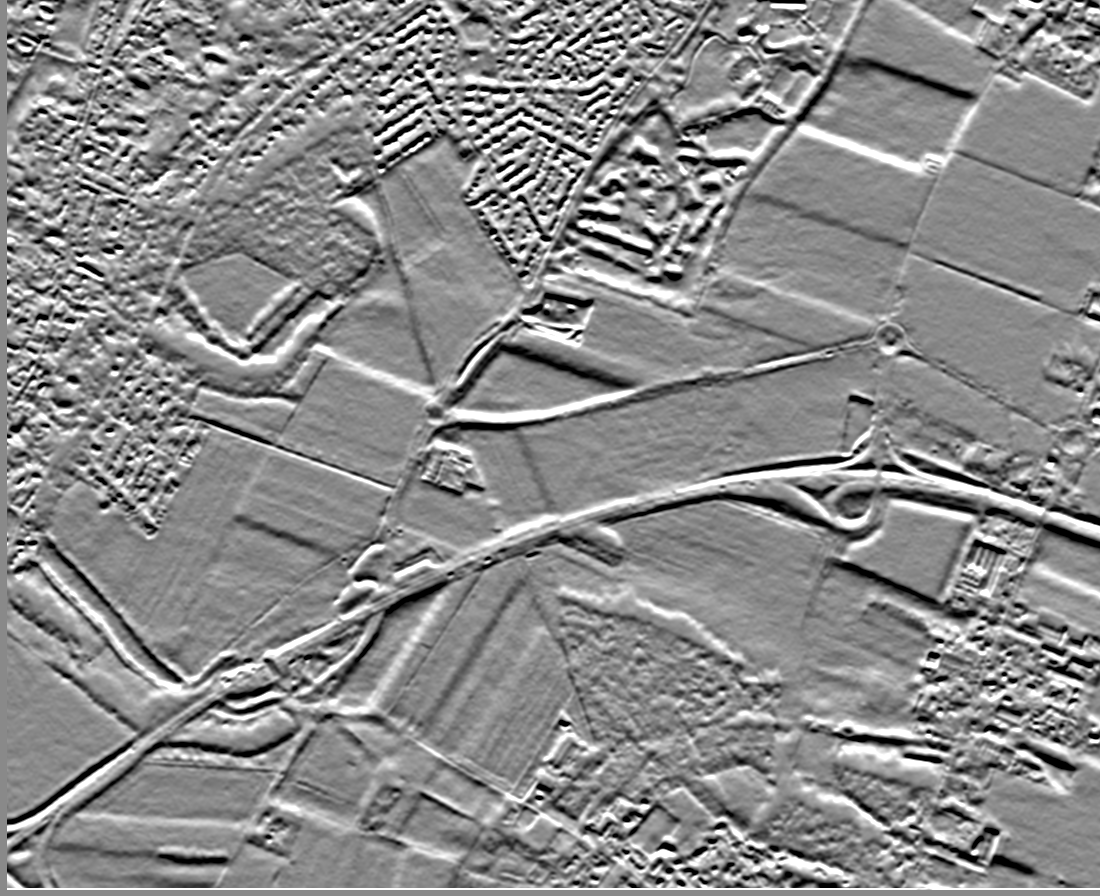
\includegraphics[scale=0.15]{Gradiente_rispetto_y}}
\caption{Calcolo del gradiente per righe e per colonne dell'immagine di test}
\label{fig:immagine_gradienti}
\end{figure}

Nel caso di immagini bidimensionali, approssimazioni di queste funzioni derivative possono essere definite al variare del grado di accuratezza. Il seguente schema evidenzia uno dei metodi di approssimazione più comune:
\begin{figure}[!ht]
\center
\begin{tikzpicture}[node distance = 3cm,]
    % Place nodes
    \node [] (input_image) {$I(j,k)$};
    \node [right of=input_image, node distance=1.5cm] (node1) {};
    \node [block, above right of=node1,  node distance=2.5cm] (gradiente_x) {Gradiente rispetto a $x$};
     \node [block, below right of=node1, node distance=2.5cm] (gradiente_y) {Gradiente rispetto a $y$};
     \node [below right  of=gradiente_x, node distance=2.5cm] (node2) {};
    \node [block, right of=node2] (combinazione) {Combinazione derivate};
    \node[right of = combinazione](uscita){$\mathbf{G}(j,k)$};
%    \node [block, right of=pesatura_bins] (normalizzazione_blocco) {\footnotesize Normalizzazione\\ contrasto};
%    \node [block, right of=normalizzazione_blocco] (features) {\footnotesize Costruzione vettore delle features};
%    \node [ below of=features,node distance=1.5cm] (classificatore) {\footnotesize Classificatore};

    % Draw edges
    \path [line] (input_image) -- (node1);
    \path [line] (node1) |- (gradiente_x);
    \path [line] (node1) |- (gradiente_y);
    \path [line] (gradiente_x) -| (node2);
    \path [line] (gradiente_y) -| (node2);
     \path [line] (node2) -- (combinazione);
     \path [line] (combinazione) -- (uscita);
     

\end{tikzpicture}

\caption{Schema di approssimazione del gradiente di un'immagine}
\label{fig:approssimazione_gradiente}
\end{figure}

La stima di $G_{x}$ e $G_{y}$ si ottiene dall'espressione della derivata monodimensionale limitata ad un piccolo intorno (spesso solo 3 punti).
L'approccio più semplice utilizza una risposta all'impulso monodimensionale di tipo $\left [\begin{matrix}-1 & 0 & 1\end{matrix}\right ]$.\\

Dal momento che la derivata, soprattutto quando calcolata su un intervallo così breve, è molto sensibile al rumore, si usa mediare in direzione ortogonale prima di effettuare la differenza per stabilizzarla. 
Con l'operatore di Prewitt, ad esempio, $G_{y}$ viene stimata mediante la differenza in orizzontale della media in verticale calcolata su tre punti.
Nella Tabella \ref{tab:gradiente} sono riassunti le varianti più comuni.

\begin{table}
\label{tab:gradiente}
\center
\caption{Operatori derivativi più usati per il calcolo del gradiente}
\begin{tabular}{ccc}
 &&\\  
 & Gradiente per riga & Gradiente per colonna \\
 &&\\ 
Roberts & $\left [\begin{matrix}
0 & 0 & -1\\

0 & 1 & 0\\

0  & 0 & 0\\
\end{matrix}\right ]$& $\left[ \begin{matrix}
-1 & 0 & 0\\

0 & 1 & 0\\

0  & 0 & 0\\
\end{matrix}\right ] $ \\ 
&&\\
Prewitt
&
$\frac{1}{3}\left [
\begin{matrix}
1& 0 &-1\\
1 &0& -1\\
1 &0& -1\\
\end{matrix}\right ]$
&
$\frac{1}{3}\left [\begin{matrix}
-1 &-1& -1\\
0  &0&  0\\
1  &1&  1\\
\end{matrix}\right ]$\\
&&\\
Sobel
&
$\frac{1}{4}\left [
\begin{matrix}
-1& -2 &-1\\
0 & 0 & 0\\
1 & 2 & 1\\
\end{matrix}\right ]$
&
$\frac{1}{4}\left [\begin{matrix}
1 & 0 & -1\\
2 & 0 & -2\\
1 & 0 & -1\\
\end{matrix}\right ]$\\
&&\\
\end{tabular} 
\end{table}

Questi operatori forniscono risultati accettabili solo per immagini poco rumorose, infatti è opportuno che l'immagine, come introdotto precedentemente, in ingresso sia filtrata al fine di limitare gli effetti del rumore.
\\

Siano $G_{x}$ e $G_{y}$ le immagini gradiente generate da:
\begin{equation}
\label{eq:gradiente_su_x}
G_{x}(j,k)= Img(j,k) * h_{x}(j,k)
\end{equation}
\begin{equation}
\label{eq:gradiente_su_y}
G_{y}(j,k)=Img(j,k) * h_{y}(j,k)
\end{equation}
dove * rappresenta la convoluzione e dove $h_{x}$ e $h_{y}$ rappresentano rispettivamente la maschera per riga e per colonna scelta tra gli operatori descritti precedentemente.
Modulo e fase del gradiente si ottengono, per ogni pixel dell'immagine, combinando $G_{x}$ e $G_{y}$ rispettivamente come:
\begin{equation}
\label{eq:"Forza_del_contorno"}
G(j,k)= \sqrt{(G_{x}(j,k))^2 + (G_{y}(j,k))^2}
\end{equation}
\begin{equation}
\label{eq:"Direzione_del_contorno"}
\theta(j,k)= atan\left (\frac{G_{y}(j,k)}{G_{x}(j,k)}\right )
\end{equation}
Per alcune applicazioni, il segno del gradiente, e quindi il valore di $\theta$ compreso tra $[0,2\pi]$ è rilevante per il problema di classificazione. Nella maggior parte delle applicazioni però, il segno del gradiente fornisce informazioni secondarie e irrilevanti; dunque $\theta(j,k)$ può essere calcolato nell'intervallo $[0,\pi]$.\\


\section{Costruzione degli istogrammi}
Il passo successivo al calcolo dei gradienti è quello di costruire gli istogrammi. A tale fine l'immagine di ingresso viene divisa in "celle" che possono essere di due diverse forme geometriche: rettangolari (R-HOG), di dimensioni $N\times N $ pixel, o circolari (C-HOG), di raggio $N$ pixel.\\
Per ogni cella viene creato un istogramma accumulando all'interno dei canali i voti dei gradienti di ciascun pixel della cella, pesati in base al modulo del gradiente. 
Gli \emph{orientation bins} sono spaziati uniformemente nell'intervallo $[0, 2\pi]$ (gradiente con segno) o $[0, \pi]$ (gradiente senza segno).\\ 
Si considerino $n_{\theta}$ \emph{angle bins} tra $[0,\pi]$ (o, come discusso in precedenza, potenzialmente, tra $[0,2\pi]$).
I descrittori HOG racchiudono le statistiche locali dei gradienti (modulo e fase) in quanto ogni pixel dà il suo voto ad uno specifico \emph{angle bin} il cui peso è proporzionale alla magnitudine del gradiente in quel determinato pixel. 
\\
Detto $ n_{\theta}$ il numero di \emph{angle bins} e posto ${\phi_{k}}={\frac{180 \cdot k}{n_{\theta}}}$, con $k=0...n_{\theta}$, e dette $n_{x}$ e $n_{y}$ il numero di celle rispettivamente sulla riga e sulla colonna dell'immagine, si costruisce una matrice tridimensionale di dimensione $n_{x}\times n_{y} \times n_{\theta}$ data da:
\begin{equation}
\label{eq:euquazione_matrice_voti}
V(i,j,k)=f\left [G(i,j)\right ]\delta(\phi_{k-1} <\theta(i,j) \leq\phi_{k}), \quad \text{con} \quad k=1,\ldots,n_{\theta}
\end{equation}
dove $ \delta(x)$ restituisce $1$ quando l'argomento è vero, $0$ quando è falso e $f$ è una funzione del modulo del gradiente (lineare, radice quadrata, quadrato o una forma saturata tra quelle riportate per rappresentare la presenza o assenza di contorni).

Un'istogramma con $n_{\theta}$ canali (\emph{orientations bins}) ad esempio è costruito nel modo seguente.
\begin{itemize} 
 \item i voti di tutti i gradienti della celle che hanno un angolo compreso nell'intervallo $\left [0, \frac{180}{n_{\theta}}\right )$ sono accumulati nel primo canale;
 \item i voti di tutti i gradienti della celle che hanno un angolo compreso nell'intervallo $\left [\frac{180}{n_{\theta}}, \frac{180}{n_{\theta}}\cdot 2\right )$ sono accumulati nel secondo canale;
 \item i voti di tutti i gradienti della celle che hanno un angolo compreso nell'intervallo $\left [\frac{180}{n_{\theta}}\cdot 2,\frac{180}{n_{\theta}}\cdot 3\right )$ sono accumulati nel terzo canale;
 \item[] $\vdots$
 \item fino al canale $n_{\theta}$ dove sono accumulati i gradienti delle celle che hanno angolo compreso tra $\left [\frac{180}{n_{\theta}}\cdot {k-1},\frac{180}{n_{\theta}}\cdot k\right )$
 \end{itemize}

Il voto dato da ciascun pixel è proporzionale alla magnitudine del gradiente di quel punto, poiché risulta importante associare ad ogni orientazione del gradiente in un dato intervallo un voto che tenga conto dell'importanza del gradiente in un determinato pixel. 
Infatti, il gradiente calcolato attorno a un bordo risulta molto più significativo di quello calcolato in una zona uniforme dell'immagine ed è essenziale per estrarre informazioni utili ad avere una descrizione dettagliata delle strutture geometriche presenti. 

\section{Normalizzazione dei blocchi}
La magnitudine del gradiente utilizzata nei descrittori HOG è sensibile ai cambiamenti locali in ambienti luminosi.
Per questo motivo è essenziale per il raggiungimento di elevate prestazioni eseguire una normalizzazione dell'istogramma, così da introdurre una migliore invarianza a diverse condizioni di luminosità, contrasto, ombre.\\
In questa fase ogni istogramma è dunque normalizzato separatamente in base ad un fattore di normalizzazione calcolato sulla base di raggruppamenti di celle circostanti, denominati "blocchi". Ognuno di questi blocchi è composto da $M \times M$ celle.

\subsection{Schemi di normalizzazione dei blocchi}
Si possono valutare diversi schemi per calcolare il valore di normalizzazione. \\
Detto $\textbf{v}$ il vettore descrittore non ancora normalizzato e sia ${\|\textbf{v}\|}_{k}$ la sua norma $k$-esima, con $k=1,2$, si possono utilizzare i seguenti schemi come proposto da Dalal e Triggs \citep{Art_HOGHuman}:
\begin{itemize}
\item L1-Norm : $\textbf{v} =\frac{\textbf{v}}{{\|\textbf{v}\|}_{1}+\varepsilon} $
\item L2-Norm :  $\textbf{v} =\frac{\textbf{v}}{{\|\textbf{v}\|}_{2}^2}+{\varepsilon}^2 $
\end{itemize}
dove $\varepsilon$ è una costante introdotta per evitare la divisione per zero e sufficientemente piccola da non alterare significativamente il risultato.
\\
Un altro metodo per effettuare la normalizzazione è quello proposto da Torrione e Morton \citep{Art_HOGLandmine}. \\
Detta $N(c)$ l'insieme di celle comprese nel blocco di interesse, il valore di normalizzazione può essere calcolato come segue:
\begin{equation}
\label{eq:normalizzazione}
H(c,k)= \frac{H_{1}(c,k)}{\left ( \sum_{c_i\in N(c)} \sqrt{\|H_{1}(c_i)\|^2_2+\varepsilon^2}\right )}
\end{equation}
dove $H_1(c,k)=\sum_{(i,j)\in c}V(i,j,k)$ e $H_1(c)$ rappresenta il vettore colonna\\
 $[H_1(c,1),\ldots, H_1(c,n_{\theta}) ]^T$.
 
 \section{Costruzione del vettore delle feature}
A questo punto si procede alla costruzione del descrittore vettoriale (\emph{feature vector}), che verrà classificato mediante un classificatore. Il descrittore avrà le stesse dimensioni dell'immagine originale con un numero di bande pari a $C + C\times B$, dove $C$ è il numero di canali dell'immagine da classificare e $B$ il numero di \emph{bins} scelto nella fase di costruzione degli istogrammi.\\
Tenendo ben presente che per immagini multispettrali l'HOG viene calcolato separatamente per ogni canale, la costruzione dei vettori delle \emph{feauture} avviene nel modo seguente: per ogni pixel vengono concatenati l'immagine originale a $C$ canali con i $C$ istogrammi, costituiti da $B$ canali, relativi a ciascuna cella e alla banda corrispondente.\\
Matematicamente, detto $\textbf{X}_{i}$ il vettore delle \emph{feature} corrispondente all' i-esimo pixel dell'immagine:
\begin{equation}
\label{eq:feature_vector}
\textbf{X}_{i}=\left[\textbf{X}_{RGB_{i}}, \textbf{f}(\textbf{X}_{RGB_{i}})\right]
\end{equation}
con \begin{equation}
\label{eq:}
\textbf{f}(\cdot)=(\textbf{f}_1,\textbf{f}_2,\ldots,\textbf{f}_k)
\end{equation}
dove $\textbf{f}_k$ è la fuzione HOG calcolata sulla singola banda k-esima e $\textbf{X}_{RGB}$ è l'immagine originale.
\\
\begin{figure}[!ht]
\centering
\begin{tikzpicture}
%\draw[color=gray!20] (0,0) grid (10,10);
%\draw[](0,0)--(5,0);
%\draw[](0,0)--(-1.25,-2.5);   
  
  %% griglia di pixel  
  \foreach \x in {0,0.25,0.5,...,5} \draw[color=blue!10,very thin] (\x,0)--+(-1.5,-1.5);
  \foreach \x in {0,5} \draw[color=blue,very thin] (\x,0)--+(-1.5,-1.5);
  
 \foreach \y in {0,0.15,0.3,...,1.6 } \draw[color=blue!10,very thin] (-1*\y,-\y)--+(5,0);
 \foreach \y in {0,1.5 } \draw[color=blue,very thin] (-1*\y,-\y)--+(5,0);
 
 \node[] at (5,-1){Immagine};
%  
%  %% griglia di celle
	\foreach \x in {0,0.5,1,...,5} \draw[color=green!60!black!20,thin] (\x+0.2,0+1)--+(-1.5,-1.5);
  \foreach \x in {0,5} \draw[color=green!60!black,thin] (\x+0.2,0+1)--+(-1.5,-1.5);
  
 \foreach \y in {0,0.3,0.6,...,1.6 } \draw[color=green!60!black!20,thin] (-1*\y+0.2,-\y+1)--+(5,0);
 \foreach \y in {0,1.5 } \draw[color=green!60!black,thin] (-1*\y+0.2,-\y+1)--+(5,0);
  \node[] at (6.1,0.25){Matrice di celle};
 %griglia di blocchi
	\foreach \x in {0,1,2,...,5} \draw[color=red!30,thin] (\x,0+2)--+(-1.2,-1.2);
  \foreach \x in {0,5} \draw[color=red,thin] (\x,0+2)--+(-1.2,-1.2);
  
 \foreach \y in {0,0.6,1.2 } \draw[color=red!30,thin] (-1*\y,-\y+2)--+(5,0);
 \foreach \y in {0,1.2 } \draw[color=red,thin] (-1*\y,-\y+2)--+(5,0);
  \node[] at (6.3,1.5){Matrice di blocchi};

	\draw[-latex](0.3,0.85)--+(-2,2);  	
	\draw[-latex](-3,3)--+(2,0);
	\draw[-latex](-3,3)--+(0,1);
	\draw[](-3,3.5)--+(0.3,0)--+(0.3,0.2)--+(0.6,0.2)--+(0.6,-.2)--+(0.9,-.2)--+(0.9,.4)--+(1.2,.4)--+(1.2,0)--+(1.5,0);
	
%	
%	
	\draw[-latex](0.75,0.85)--+(0,1.5);  
	\draw[-latex](0.,2.5)--+(2,0);
  	\draw[-latex](0.,2.5)--+(0,1);
  	\draw[](0,3)--+(0.3,0)--+(0.3,0.2)--+(0.6,0.2)--+(0.6,-.2)--+(0.9,-.2)--+(0.9,.4)--+(1.2,.4)--+(1.2,0)--+(1.5,0);
  	\node[] at (0,4){Istogrammi};
  \end{tikzpicture}
\caption{Schema esemplificativo della distribuzione spaziale di istogrammi, celle e blocchi}
\label{fig:HOG_Schema}
\end{figure}

%
%\chapter{Valutazione delle Prestazione del classificatore}
%
%\label{prestazioni_capitolo} % Change X to a consecutive number; for referencing this chapter elsewhere, use \ref{ChapterX}
%
%%\lhead{Capitolo \ref{prestazioni_capitolo}. \emph{Valutazione delle prestazioni del classificatore}} % Change X to a consecutive number; this is for the header on each page - perhaps a shortened title
%
%%----------------------------------------------------------------------------------------
%%	SECTION 1
%%----------------------------------------------------------------------------------------
%
%
%Dato un classificatore supervisionato, addestrato su un training set, è fondamentale saper valutare l'accuratezza che può essere ottenuta quando tale classificatore è applicato a valori incogniti.\\
%A tale scopo è essenziale valutare la probabilità di errore $P_e$ del classificatore, per decidere, ad esempio, se le \emph{feature} utilizzate siano sufficienti a discriminare bene le classi o se sia necessario estrarne altre (come parametri di tessitura nel caso in cui i canali spettrali non siano abbastanza discriminanti).
%\clearpage
%
%\subsection{Stima della probabilità di errore}
%In presenza di $C$ classi $\omega_1,\omega_2, \ldots, \omega_C$, detta $P_i$ la probabilità di errore \emph{a priori}, la probabilità di errore $P_e$ si può esprimere nel modo seguente:
%\begin{equation}
%\label{eq:P_e}
%P_e = P\lbrace\widehat{Y}\neq Y\rbrace= {\sum_{i=1}^C P\lbrace\widehat{Y}\neq \omega_i\vert Y = \omega_i\rbrace}P\lbrace Y =\omega_i\rbrace
%\end{equation}
%Dal momento che tale espressione è calcolabile solo in pochissimi casi semplici, per valutarla si adotta generalmente un approccio empirico, che stima la $P_e$ come la percentuale dei pixel di test classificati erroneamente.\\
%Solitamente la $P_e$ viene valutata su un insieme di campioni pre-etichettati(\emph{test set}) diverso rispetto a quello utilizzato per addestrare il classificatore(\emph{training set}). Questa tecnica, detta \emph{hold-out}, permette una misura delle prestazioni priva di \emph{bias} in quanto eseguita su istanze non utilizzate in fase di apprendimento.\\
%Per evitare il fenomeno dell'overfitting,\footnote{Si parla di overfitting quando la funzione discriminante è strettamente dipendente dai campioni di training specifici utilizzati per calcolarla ed è quindi particolarmente inefficace quando applicata a campioni incogniti} un'ipotesi fondamentale per stimare $P_e$ come frequenza relativa degli errori sul test set è che i campioni pre-etichettati siano indipendenti e identicamente distribuiti (i.i.d). Per questa ragione è buona norma prelevare i campioni di \emph{training} e di \emph{test} in regioni dell'immagine spazialmente disgiunte tra loro.\\
%E' altrettanto importante effettuare un'analisi qualitativa dell'intera mappa, mediante foto-interpretazione, come complemento alla valutazione quantitativa delle prestazioni di classificazione sui campioni di test.
%
%\subsection{Matrice di confusione e parametri di accuratezza}
%La $P_e$ fornisce una valutazione complessiva delle prestazioni del classificatore, senza però differenziare gli errori commessi in corrispondenza di classi diverse. Per una valutazione più dettagliata la matrice di confusione (confusion matrix) è la tipologia di osservazione statistica maggiormente utilizzata: il risultato della classificazione sulle aree campione viene confrontato con la verità al suolo [Congalton]. Questa è una matrice $C \times C$, il cui elemento $e_{ij}$ è il numero di pixel di test della classe $\omega_i$ che il classificatore ha assegnato alla classe $\omega_j$. Sulla diagonale $i=j$ della matrice di confusione si leggono dunque i numeri di pixel di test classificati in modo corretto. Questo tipo di analisi statistica consente non solo di quantificare il successo ottenuto dalla procedura, ma anche di focalizzare i punti critici del processo di classificazione, ovvero le classi meno distinguibili tra loro. \\
%L'accuratezza della classificazione può essere valutata con diversi parametri numerici, tra cui i più utilizzati sono:
%\begin{itemize}
%\item L' \emph{average accuracy} (AA) delle C classi è la media rispetto al numero di classi delle frazioni di pixel correttamente classificati (classe per classe), ed è data da:
%\begin{equation}
%\label{eq:AA}
%AA=\dfrac{1}{C}\sum_{i=1}^C\dfrac{e_{ij}}{\sum_{j=1}^C e_{ij}}
%\end{equation}
%\item L'\emph{overall accuracy }(OA) è la percentuale di pixel ben classificati sull'intero test set ed è data da:
%\begin{equation}
%\label{eq:OA}
%OA= \dfrac{1}{t}\sum_{i=1}^C e_{ij}
%\end{equation}
%\item Il parametro "$\kappa$", rappresenta una modifica dell' OA finalizzata a tenere conto in modo più completo della distribuzione degli errori tra le diverse classi, ed è dato da:
%\begin{equation}
%\label{eq:K}
%\kappa=\dfrac{OA-\frac{1}{t^2}\sum_{i=1}^C\sum_{j=1}^C\sum_{k=1}^C e_{ij}e_{ki}}{1-\frac{1}{t^2}\sum_{i=1}^C\sum_{j=1}^C\sum_{k=1}^C e_{ij} e_{ki}}
%\end{equation}
%dove t è il numero di pixel di test.
%\end{itemize}

% Chapter Template
% !TEX root = ../main.tex
\chapter{SVM - \emph{Support Vector Machine}} % Main chapter title

\label{cap:svm} % Change X to a consecutive number; for referencing this chapter elsewhere, use \ref{ChapterX}

Una SVM (\emph{Support Vector Machine}) è un modello di apprendimento supervisionato associato ad algoritmi largamente utilizzati per il \emph{data analysis} e il \emph{pattern recognition} (tra cui anche il problema della classificazione).
L'SVM è un modello abbastanza recente; anche se la sua formulazione risale agli anni '60, solo negli ultimi 15/20 anni si è registrato un incremento significativo nell'uso di algoritmi SVM per classificazione.
La sua fortuna risiede nel fatto che può essere facilmente esteso in molti campi, senza stravolgere la semplicità che caratterizza questi classificatori.
\\
Questo capitolo servirà per introdurre la teoria matematica su cui si basa un classificatore SVM e sarà impostato nel seguente modo: si inizierà descrivendo dettagliatamente il modello più semplice di SVM (SVM lineare per classificazione binaria), poi si proseguirà con la descrizione di come è possibile estendere questo modello per una classificazione non-lineare e, infine, verranno introdotte le possibili modifiche che permettono la classificazione multiclasse.
\clearpage

\section{SVM lineare per classificazione binaria}
Dato un \emph{training set} linearmente separabile $(\mathbf{x}_i,y_i)$, $i=1,\ldots,N$, con $\mathbf{x}_i\in\mathbb{R}^d$ e $y_i\in\left\lbrace -1,1\right\rbrace$, l'obiettivo è addestrare un classificatore affinché
\begin{equation}
\label{eq:SVM_lin_bin}
f(\mathbf{x}_i):\twopartdef{>0}{y_i=+1}{< 0}{y_i=-1}
\end{equation}
ovvero $y_if(\mathbf{x}_i)>0$ per una corretta classificazione.
La funzione $f$ è detta \textit{regola di decisione} ed è costruita in modo tale che, preso un qualsiasi \textit{campione incognito} $\mathbf{u}$ da classificare, il valore di $f$ valutato in $\mathbf{u}$ restituisce una stima dell'etichetta $y_u$ da associare. In equazioni:
\begin{equation}
\label{eq:regola_di_decisione}
f\text{ tale che }
\left\{
		\begin{array}{ll}
			\text{Se } f(\mathbf{u})>0 & \mbox{allora } y_u=+1 \\
			\text{Se } f(\mathbf{u})<0 & \mbox{allora } y_u=-1 \\
		\end{array}
	\right.
\end{equation}
\subsection{Hard Margin SVM}
Un insieme di elementi in $\mathbb{R}^d$ è linearmente separabile se esiste almeno un iperpiano (che in generale avrà dimensione $d-1$) in grado di separare, nello spazio vettoriale dei campioni in ingresso, quelli che richiedono un'etichetta positiva da quelli che richiedono un'etichetta negativa. 
\\
Si prenda, per esempio, la situazione proposta in Figura \ref{fig:insieme_lin_separ}: qui si può facilmente evincere che esiste almeno un iperpiano (in questo caso una retta) che divida lo spazio in due semispazi, ciascuno dei quali contiene campioni di una sola classe.
\begin{figure}[!ht]
\begin{center}

	\begin{tikzpicture}[scale=0.8]
	  % Draw axes
	 \draw [] (0,5) node (yaxis) [above] {$x_2$}
	        |- (5,0) node (xaxis) [right] {$x_1$};
	  \draw (0,-1) -- (5,4);
	  \draw (2,-1) -- (3,5);
	  % Draw negative dots
	  	\fill[black] (0.5,1.5) circle (3pt);
	  	\fill[black]   (1.5,2.5)   circle (3pt);
	  	\fill[black] (1,2.5)     circle (3pt);
	  	\fill[black] (0.75,2)    circle (3pt);
	  	\fill[black] (0.6,1.9)   circle (3pt);
	  	\fill[black] (0.77, 2.5) circle (3pt);
	  	\fill[black] (1.5,3)     circle (3pt);
	  	\fill[black] (1.3,3.3)   circle (3pt);
	  	\fill[black] (0.6,3.2)   circle (3pt);
	  % Draw positive dots
  		\draw[black,thick] (4,1)     circle (3pt); 
  		\draw[black,thick] (3.3,.3)  circle (3pt); 
  		\draw[black]     (4.5,1.2) circle (3pt); 
  		\draw[black]     (4.5,.5)  circle (3pt); 
  		\draw[black]     (3.9,.7)  circle (3pt); 
  		\draw[black]     (5,1)     circle (3pt); 
  		\draw[black]     (3.5,.2)  circle (3pt); 
  		\draw[black]     (4,.3)    circle (3pt); 
	\end{tikzpicture}
	
\end{center}
	\caption{Dataset linearmente separabile}
	\label{fig:insieme_lin_separ}
\end{figure}
\\
Il problema nasce dal fatto che possono esistere infiniti iperpiani e la scelta di quale usare per l'addestramento potrebbe avere ripercussioni notevoli per la fase di classificazione. 
L'SVM risolve questo problema cercando l'iperpiano che massimizza il margine tra i due insiemi di elementi. 
\\
In termini più matematici, un iperpiano in $\mathbb{R}^d$ ha forma:
\begin{equation}
\label{eq:iperpiano}
\mathbf{w}\cdot\mathbf{x}+b=0
\end{equation}
dove $\mathbf{w}\in\mathbb{R}^d$ è la normale all'iperpiano e $b/ \vert\vert\mathbf{w}\vert\vert$ è la distanza perpendicolare dall'iperpiano all'origine.
\\
Alla luce di ciò, si può riscrivere la \textit{regola di decisione} presentata nell'equazione (\ref{eq:regola_di_decisione}) nel seguente modo:
\begin{equation}
\label{eq:regola_di_decisioneSVM}
\left\{
		\begin{array}{ll}
			\text{Se } \mathbf{w}\cdot\mathbf{u}+b>0 & \mbox{allora } y_u=+1 \\
			\text{Se } \mathbf{w}\cdot\mathbf{u}+b<0 & \mbox{allora } y_u=-1 \\
		\end{array}
	\right.
\end{equation}

Dato che $\mathbf{w}\cdot\mathbf{x}+b=0$ e $c\left (\mathbf{w}\cdot\mathbf{x}+b\right )=0$ definiscono la stessa regola di decisione (per $c>0$), si ha libertà di scegliere la normalizzazione di $\mathbf{w}$.
In questo caso, si può scegliere il fattore di normalizzazione in modo tale che $\mathbf{w}\cdot\mathbf{x}_i+b\geq 1$ e $\mathbf{w}\cdot\mathbf{x}_i+b\leq-1$, per gli elementi della prima classe e della seconda rispettivamente.
Per convenienza matematica, dato che $y_i\in\left\lbrace -1,1\right\rbrace$, le due identità precedenti possono essere riscritte nel seguente modo:
\begin{equation}
\label{eq:disq_elementi1}
y_i\left (\mathbf{w}\cdot\mathbf{x}_i+b\right )\geq1,\quad \forall i=1,\ldots,N
\end{equation}
o, analogamente,
\begin{equation}
\label{eq:disq_elementi2}
y_i\left (\mathbf{w}\cdot\mathbf{x}_i+b\right )-1\geq0,\quad \forall i=1,\ldots,N
\end{equation}
con l'uguaglianza valida per gli elementi sul bordo (i punti rossi in Figura \ref{fig:margine}).
\\

\begin{figure}[!ht]
\begin{center}

	\begin{tikzpicture}
  % Draw axes
 \draw [] (0,5) node (yaxis) [above] {$x_2$}
        |- (5,0) node (xaxis) [right] {$x_1$};
  % Draw line
  \draw (0,-1) -- (5,4); % y=x-1
  \draw[dashed] (-1,0) -- (4,5); % y=x+1
  \draw[dashed] (2,-1) -- (6,3); % y=x-3
%  % Draw labels
  \draw (3.5,3) node[rotate=45] 
        {$\mathbf{w}\cdot \mathbf{x} + b = 0$};
  \draw (2.5,4) node[rotate=45] 
        {$\mathbf{w}\cdot \mathbf{x}_+ + b = 1$};
  \draw (4.5,2) node[rotate=45] 
       {$\mathbf{w}\cdot \mathbf{x}_- + b = -1$};
  % Draw distance
  \draw[dotted] (4,5) -- (6,3);
  \draw (5.25,4.25) node[rotate=-45] {$\frac{2}{\Vert \mathbf{w} \Vert}$};
  \draw[dotted] (0,0) -- (0.5,-0.5);
  \draw (0,-0.5) node[rotate=-45] {$\frac{b}{\Vert \mathbf{w} \Vert}$};
  \draw[-latex] (2,1) -- (1.5,1.5);
  \draw (1.85,1.35) node[rotate=-45] {$\mathbf{w}$};
  % Draw negative dots
  \fill[red] (0.5,1.5) circle (3pt);
  \fill[red]   (1.5,2.5)   circle (3pt);
  \fill[black] (1,2.5)     circle (3pt);
  \fill[black] (0.75,2)    circle (3pt);
  \fill[black] (0.6,1.9)   circle (3pt);
  \fill[black] (0.77, 2.5) circle (3pt);
  \fill[black] (1.5,3)     circle (3pt);
  \fill[black] (1.3,3.3)   circle (3pt);
  \fill[black] (0.6,3.2)   circle (3pt);
  % Draw positive dots
  \draw[red,thick] (4,1)     circle (3pt); 
  \draw[red,thick] (3.3,.3)  circle (3pt); 
  \draw[black]     (4.5,1.2) circle (3pt); 
  \draw[black]     (4.5,.5)  circle (3pt); 
  \draw[black]     (3.9,.7)  circle (3pt); 
  \draw[black]     (5,1)     circle (3pt); 
  \draw[black]     (3.5,.2)  circle (3pt); 
  \draw[black]     (4,.3)    circle (3pt); 
\end{tikzpicture}
	
\end{center}
	\caption{Margine tra i campioni di \emph{training} di due classi linearmente separabili}
	\label{fig:margine}
\end{figure}

Geometricamente, sotto queste ipotesi, si dimostra che il margine risulta essere: 
\begin{equation}
\label{eq:margine}
\dfrac{\mathbf{w}}{\vert\vert\mathbf{w}\vert\vert}\cdot\left (\mathbf{x}_+-\mathbf{x}_-\right )=\dfrac{2}{\vert\vert\mathbf{w}\vert\vert}
\end{equation}
dove $\mathbf{x}_+$ e $\mathbf{x}_-$ sono i campioni delle due classi (rispettivamente) più vicini al iperpiano separatore (vedi Figura \ref{fig:margine} ed equazione (\ref{eq:disq_elementi2})).
\\
L'obiettivo ora è quindi massimizzare questo valore, che equivale a minimizzare $\vert\vert\mathbf{w}\vert\vert$, il quale, a sua volta, per convenienza matematica, può essere espresso nel seguente termine:
\begin{eqnarray}\nonumber
\label{eq:problema_di_minimizzazione}
&\text{min}\dfrac{1}{2}\vert\vert\mathbf{w}\vert\vert^2\\
&\text{ vincolato a }y_i\left (\mathbf{w}\cdot\mathbf{x}_i+b\right )-1=0 \quad \forall i=1,\ldots,N
\end{eqnarray}
%\begin{equation}
%\label{eq:problema_di_minimizzazione}
%\text{min}\dfrac{1}{2}\vert\vert\mathbf{w}\vert\vert^2
%\text{ vincolato a }y_i\left (\mathbf{w}\cdot\mathbf{x}_i+b\right )-1=0
%\end{equation}
\\
%Discorso sul problema della programmazione quadratica.
%(Poiché questi problemi sono già stati ampiamente studiati sia dal punto di vista teorico che da quello applicativo degli algoritmi, possiamo beneficiare immediatamente dei risultati ottenuti nella teoria dell’ottimizzazione. In particolare, questo approccio produce algoritmi computazionalmente efficienti e adattabili a un ampio numero di casi in cui non i dati non sono classificabili senza errore.
%Because it is quadratic, the surface is a paraboloid, with just a single global minimum 
%\\
Essendo questo un chiaro esempio di calcolo di estremi vincolati, per semplificare i calcoli, si possono usare i \textit{Moltiplicatori di Lagrange}, che permettono di lavorare su un problema duale, ovvero l'ottimizzazione (minimizzazione rispetto a $\mathbf{w}$ e a $b$) della seguente funzione:
\begin{equation}
\label{eq:lagrangiana}
\text{min}_{\mathbf{w},b}\text{ }L=\dfrac{1}{2}\vert\vert\mathbf{w}\vert\vert^2-\sum_i\alpha_i\left [y_i\left (\mathbf{w}\cdot\mathbf{x}_i+b\right )-1\right ]
\end{equation}
dove si sottintende, da questo punto, che la sommatoria sia per ogni $i=1,\ldots,N$.
\\
Procedendo con il calcolo del gradiente di $L$ si ottengono i seguenti risultati:
\begin{equation}
\label{eq:deriv_lagrang_rispetto_w}
\dfrac{\partial L}{\partial \mathbf{w}}=\mathbf{w}-\sum_i\alpha_i y_i\mathbf{x}_i=0 \quad\Rightarrow\quad \mathbf{w}=\sum_i\alpha_i y_i\mathbf{x}_i
\end{equation}
\begin{equation}
\label{eq:deriv_lagrang_rispetto_b}
\dfrac{\partial L}{\partial b}=-\sum_i\alpha_iy_i=0 \quad\Rightarrow\quad \sum_i\alpha_iy_i=0
\end{equation}
L'equazione (\ref{eq:deriv_lagrang_rispetto_w}) suggerisce che il vettore $\mathbf{w}$ non sia altro che una combinazione lineare di alcuni vettori di \emph{training} (per alcuni di loro $\alpha_i$ sarà pari a $0$), mentre l'equazione (\ref{eq:deriv_lagrang_rispetto_b}) sarà utile più avanti.

A questo punto si introduce il cosiddetto \textit{Problema lagrangiano duale}: invece di \emph{minimizzare} rispetto a $\mathbf{w}$ e $b$, si può \emph{massimizzare} rispetto ad $\alpha$ con vincoli le relazioni ottenute precedentemente per $\mathbf{w}$ e $b$ (equazioni (\ref{eq:deriv_lagrang_rispetto_w}) e (\ref{eq:deriv_lagrang_rispetto_b}))\footnote{Il teorema di Kunh-Tucker assicura che la soluzione di questo problema è la stessa del problema originario.}.

Dato che l'equazione (\ref{eq:deriv_lagrang_rispetto_w}) restituisce una definizione per $\mathbf{w}$, possiamo sostituire questo risultato nella lagrangiana $L$ (eq.ne (\ref{eq:lagrangiana})), ottenendo:
\begin{eqnarray}\nonumber
\label{eq:lagrangiana_finale1}
&L(\mathbf{w},b)	= \dfrac{1}{2}\left ( \sum_i \alpha_iy_i\mathbf{x}_i \right )\cdot\left (\sum_j\alpha_jy_j\mathbf{x}_j\right )+\\
		&-\sum_i\left [\alpha_iy_i\mathbf{x}_i\cdot\left (\sum_j\alpha_jy_j\mathbf{x}_j\right )\right ]-
		\sum_i\alpha_iy_ib+\sum_i\alpha_i	
\end{eqnarray}
%\begin{equation}
%\label{eq:lagrangiana_finale1}
%L	= \dfrac{1}{2}\left ( \sum_i \alpha_iy_i\mathbf{x}_i \right )\cdot\left (\sum_j\alpha_jy_j\mathbf{x}_j\right )-
%		\sum_i\left [\alpha_iy_i\mathbf{x}_i\cdot\left (\sum_j\alpha_jy_j\mathbf{x}_j\right )\right ]-
%		\sum_i\alpha_iy_ib+\sum_i\alpha_i	
%\end{equation}
A questo punto, cambiando l'ordine delle sommatorie nel secondo membro e notando che il penultimo addendo è sempre nullo (vedi equazione (\ref{eq:deriv_lagrang_rispetto_b})), si ottiene la versione finale della lagrangiana duale: 
\begin{equation}
\label{eq:langrangiana_finale2}
L=\sum_i\alpha_i-\dfrac{1}{2	}\sum_i\sum_j\alpha_i\alpha_jy_iy_j\mathbf{x}_i\cdot\mathbf{x}_j
\end{equation}
L'equazione appena riportata è un problema di programmazione quadratica (\emph{quadratic programmimg}, QP) che assicura l'esistenza e l'unicità di una e una sola soluzione.\\

Per completare il discorso sulla SVM lineare, si consideri nuovamente la \emph{regola di decisione} introdotta nell'equazione (\ref{eq:regola_di_decisioneSVM}). Avendo ora una definizione formale per $\mathbf{w}$, questa può essere riscritta nel seguente modo:
\begin{equation}
\label{eq:regola_di_decisioneSVM_lineare}
\left\{
		\begin{array}{ll}
			\text{Se } \sum_i\alpha_i y_i\mathbf{x}_i\cdot\mathbf{u}+b>0 & \mbox{allora } y_u=+1 \\
			\text{Se } \sum_i\alpha_i y_i\mathbf{x}_i\cdot\mathbf{u}+b<0 & \mbox{allora } y_u=-1 \\
		\end{array}
	\right.
\end{equation}

Il motivo dell'uso di questo espediente matematico risiede nel fatto che adesso sia l'ottimizzazione della lagrangiana (\ref{eq:langrangiana_finale2}) sia la \emph{regola di decisione} (\ref{eq:regola_di_decisioneSVM_lineare}) dipendono esclusivamente da un prodotto scalare tra due vettori, $\mathbf{x}_i\cdot\mathbf{x}_j$ e $\mathbf{x}_i\cdot\mathbf{u}$ rispettivamente, e questo semplificherà notevolmente la trattazione della SVM non lineare. 

\subsection{Soft Margin SVM}
Prima di introdurre l'estensione della SVM che permetta la classificazione non-lineare, è interessante discutere di come sia possibile usare una SVM lineare anche per situazioni in cui il \emph{training set} non sia linearmente separabile.\\
Si prenda, come esempio, la situazione proposta di seguito (Figura \ref{fig:Dataset_nonseparabile}).
 \begin{figure}[!ht]
 \center
\begin{tikzpicture}
%\draw[step=0.5,blue!20,thin] (-1,-1) grid (6,6);
%\draw[step=1,blue!50,thin] (-1,-1) grid (6,6);
  % Draw axes
 \draw [] (0,5) node (yaxis) [above] {$x_2$}
        |- (5,0) node (xaxis) [right] {$x_1$};
  % Draw line
%  \draw (-1,-.25) -- (4,4.75); % y=x-1
%  \draw[dashed] (-1,0) -- (4,5); % y=x+1
%  \draw[dashed] (-1,-0.5) -- (4,4.5); % y=x-3 (x+2)


  % Draw negative dots
  \fill[black] (1.5,1) circle (3pt);
  \fill[black]   (2,1.5)   circle (3pt);%%
  \fill[black] (1,2.5)     circle (3pt);
  \fill[black] (0.75,2)    circle (3pt);
  \fill[black] (0.6,1.9)   circle (3pt);
  \fill[black] (0.77, 2.5) circle (3pt);
  \fill[black] (1.5,3)     circle (3pt);
  \fill[black] (1.3,3.3)   circle (3pt);
  \fill[black] (0.6,3.2)   circle (3pt);
  % Draw positive dots
  \draw[black] (1.5,2)     circle (3pt); 
  \draw[black] (3.3,.3)  circle (3pt); 
  \draw[black]     (4.5,1.2) circle (3pt); 
  \draw[black]     (4.5,.5)  circle (3pt); 
  \draw[black]     (3.9,.7)  circle (3pt); 
  \draw[black]     (5,1)     circle (3pt); 
  \draw[black]     (3.5,.2)  circle (3pt); 
  \draw[black]     (4,.3)    circle (3pt); 
\end{tikzpicture}
    \caption{Dataset non linearmente separabile}
    \label{fig:Dataset_nonseparabile}
  \end{figure}
\\
Si nota chiaramente come, in questo caso, non esista alcun iperpiano separatore. 
Nonostante ciò, modificando leggermente il modello di SVM introdotto fino a questo punto, si può dimostrare che è ancora possibile utilizzare una SVM lineare.\\

La chiave di questo nuovo modello sta nell'introduzione di una \emph{variabile slack}, in modo tale da rilassare quei vincoli rigidi che non permetterebbero l'uso di una SVM lineare. \\
Precedentemente, i margini erano definiti dei vincoli:
\begin{equation}
\label{eq:vincolo_hard_margin}
y_i\left (\mathbf{x}_i\cdot\mathbf{w}+b \right )\geq1   \quad     y_i\in\left\lbrace-1,1\right \rbrace
\end{equation}
Nella soluzione proposta, invece, sono definiti da:
\begin{equation}
\label{eq:vincolo_soft_margin}
y_i\left (\mathbf{x}_i\cdot\mathbf{w}+b \right )\geq1-\xi_i   \quad    \xi_i\geq0, y_i\in\left\lbrace-1,1\right \rbrace
\end{equation}
La situazione che si è andata a definire, graficamente, appare in Figura \ref{fig:soft_margin}.
 \begin{figure}[!ht]
\center
\begin{tikzpicture}[scale=0.9]
%\draw[step=0.5,blue!20,thin] (-1,-1) grid (6,6);
%\draw[step=1,blue!50,thin] (-1,-1) grid (6,6);
  % Draw axes
 \draw [] (0,5) node (yaxis) [above] {$x_2$}
        |- (5,0) node (xaxis) [right] {$x_1$};
  % Draw line
  \draw (0,-1) -- (5,4); % y=x-1
  \draw[dashed] (-1,0) -- (4,5); % y=x+1
  \draw[dashed] (2,-1) -- (6,3); % y=x-3

\draw[-latex](3.5,0.5)--(3,1);  
\draw[-latex](4.5,1.5)--(2,4);  
%  % Draw labels

  % Draw negative dots
  \fill[red] (0.5,1.5) circle (3pt);
  \fill[red]   (1.5,2.5)   circle (3pt);
  \fill[black] (1,2.5)     circle (3pt);
  \fill[black] (0.75,2)    circle (3pt);
  \fill[black] (0.6,1.9)   circle (3pt);
  \fill[black] (0.77, 2.5) circle (3pt);
  \fill[black] (1.5,3)     circle (3pt);
  \fill[black] (1.3,3.3)   circle (3pt);
  \fill[black] (0.6,3.2)   circle (3pt);
  % Draw positive dots
  \draw[red,thick] (4,1)     circle (3pt); 
  \draw[red,thick] (3,0)  circle (3pt)node[below right ,black]{$\xi=0$}; 
  
  \draw[red,thick] (3,1)  circle (3pt)node[above ,black]{$\xi<1$}; 
  \draw[red,thick] (2,4)  circle (3pt)node[above ,black]{$\xi>1$}; 
  \draw[black]     (4.5,1.2) circle (3pt); 
  \draw[black]     (4.5,.5)  circle (3pt); 
  \draw[black]     (3.9,.7)  circle (3pt); 
  \draw[black]     (5,1)     circle (3pt); 
  \draw[black]     (3.5,.2)  circle (3pt); 
  \draw[black]     (4,.3)    circle (3pt); 
\end{tikzpicture}
    \caption{Esempio di soft margin}
    \label{fig:soft_margin}
  \end{figure}

Il nuovo vincolo permette al margine funzionale di essere minore di 1. L'errore che si commette è, però, $C\xi_i$, sia per i punti che ricadrebbero nella parte corretta dell'iperpiano separatore ($0<\xi_i\leq1$), sia per quelli che sarebbero nel lato sbagliato ($\xi>1$).
Si sono, quindi, "rilassati" i vincoli in modo tale da classificare dati non-separabili, con una penalità linearmente proporzionale all'entità dell'errore commesso sul training set.\\

Il nuovo problema di ottimizzazione è il seguente:
\begin{eqnarray}
\label{eq:ottimizzazione_softmargin}
&\text{min }\dfrac{1}{2}\vert\vert\mathbf{w}\vert\vert^2+C\sum_i\xi_i\\
&\text{vincolato a }&y_i\left (\mathbf{x}_i\cdot\mathbf{w}+b \right )\geq1-\xi_i\\
&& \xi_i\geq0, \quad \forall i=1,\ldots,N
\end{eqnarray}
La costante $C$ (con $C\geq0$) gestisce il compromesso fra la minimizzazione dei due contributi alla funzione obiettivo: se $C=0$ gli errori sul training set non sono penalizzati; se $C$ è molto grande, il termine legato al margine è minoritario e gli errori sul training set sono molto penalizzati.
\\
Allo stesso modo del caso lineare, possono essere usati i moltiplicatori di Lagrange; la funzione da ottimizzare quindi è la seguente:
\begin{equation}
\label{eq:lagrangiana_sofmargin}
L=\dfrac{1}{2}\vert\vert\mathbf{w}\vert\vert^2+C\sum_i\xi_i+\sum_i\alpha_i\left [1-\xi_i-y_i\left (\mathbf{x}_i\cdot\mathbf{w}+b \right )\right ]-\sum_i\beta_i\xi_i
\end{equation}
dove $\beta_i$ sono i moltiplicatori di Lagrange necessari per vincolare la positività della \emph{variabile slack}.	
\\

\'E interessante notare come l'applicazione di una soft-margin SVM possa avere prestazioni migliori della hard-margin SVM anche per dataset linearmente separabili. Per chiarificarne il motivo, un esempio è riportato nella figura successiva: il training set permetterebbe l'uso di una hard-margin SVM, ma il risultato  avrebbe un margine piuttosto limitato, confrontato con quello che si otterrebbe in caso di soft-margin SVM. \\
 \begin{figure}[!ht]
 \centering
 \subfigure[Hard Margin SVM]
   {
		\begin{tikzpicture}[scale=.9]
  % Draw axes
 \draw [] (0,5) node (yaxis) [above] {$x_2$}
        |- (5,0) node (xaxis) [right] {$x_1$};
  % Draw line
  \draw (-1,-.25) -- (4,4.75); % y=x-1
  \draw[dashed] (-1,0) -- (4,5); % y=x+1
  \draw[dashed] (-1,-0.5) -- (4,4.5); % y=x-3 (x+2)

  \fill[red] (0.5,1.5) circle (3pt);
  \fill[red]   (1.5,2.5)   circle (3pt);
  \fill[black] (1,2.5)     circle (3pt);
  \fill[black] (0.75,2)    circle (3pt);
  \fill[black] (0.6,1.9)   circle (3pt);
  \fill[black] (0.77, 2.5) circle (3pt);
  \fill[black] (1.5,3)     circle (3pt);
  \fill[black] (1.3,3.3)   circle (3pt);
  \fill[black] (0.6,3.2)   circle (3pt);
  % Draw positive dots
  \draw[red,thick] (1.5,2)     circle (3pt); 
   \draw[black] (4,1)     circle (3pt);
  \draw[black] (3.3,.3)  circle (3pt); 
  \draw[black]     (4.5,1.2) circle (3pt); 
  \draw[black]     (4.5,.5)  circle (3pt); 
  \draw[black]     (3.9,.7)  circle (3pt); 
  \draw[black]     (5,1)     circle (3pt); 
  \draw[black]     (3.5,.2)  circle (3pt); 
  \draw[black]     (4,.3)    circle (3pt); 
\end{tikzpicture}   
   }
 \hspace{4mm}
 \subfigure[Soft Margin SVM]
   {
\begin{tikzpicture}[scale=.9]
  % Draw axes
 \draw [] (0,5) node (yaxis) [above] {$x_2$}
        |- (5,0) node (xaxis) [right] {$x_1$};
  % Draw line
  \draw (0,-1) -- (5,4); % y=x-1
  \draw[dashed] (-1,0) -- (4,5); % y=x+1
  \draw[dashed] (2,-1) -- (6,3); % y=x-3

  \fill[red] (0.5,1.5) circle (3pt);
  \fill[red]   (1.5,2.5)   circle (3pt);
  \fill[black] (1,2.5)     circle (3pt);
  \fill[black] (0.75,2)    circle (3pt);
  \fill[black] (0.6,1.9)   circle (3pt);
  \fill[black] (0.77, 2.5) circle (3pt);
  \fill[black] (1.5,3)     circle (3pt);
  \fill[black] (1.3,3.3)   circle (3pt);
  \fill[black] (0.6,3.2)   circle (3pt);
  % Draw positive dots
    \draw[red,thick] (4,1)     circle (3pt); %da aggiungere
  \draw[red,thick] (3.3,.3)  circle (3pt); 
  \draw[red,thick] (1.5,2)     circle (3pt); 
 
  \draw[black]     (4.5,1.2) circle (3pt); 
  \draw[black]     (4.5,.5)  circle (3pt); 
  \draw[black]     (3.9,.7)  circle (3pt); 
  \draw[black]     (5,1)     circle (3pt); 
  \draw[black]     (3.5,.2)  circle (3pt); 
  \draw[black]     (4,.3)    circle (3pt); 
\end{tikzpicture}   
   }
 \caption{Confronto di strategia tra Hard Margin SVM e Soft Margin SVM}
 \end{figure}
 
\section{SVM non lineare per classificazione binaria}
Nonostante l'introduzione della variante Soft-Margin della SVM possa il qualche caso tornare utile, può capitare che anche questa strategia sia difficilmente applicabile o produca risultati non soddisfacenti (si rimanda al Capitolo X dove si discuterà come avere una stima delle prestazioni di un classificatore).
\\

L'intento della classificazione SVM non-lineare è quello di trasformare lo spazio dei vettori di training non linearmente separabili $\mathbb{R}^d$ in uno spazio $\mathcal{H}$ (la cui dimensionalità sarà maggiore di $d$ o anche, potenzialmente, infinita) in cui i campioni siano disposti in modo tale da permettere l'utilizzo di una SVM lineare. Questo passo si giustifica tramite il \emph{Teorema di Cover sulla separabilità}, il quale afferma che un problema di classificazione complesso, formulato attraverso una trasformazione non-lineare dei dati in uno spazio ad alta dimensionalità, ha maggiore probabilità di essere linearmente separabile che in uno spazio a bassa dimensionalità.
\\
Si ricerca quindi una funzione di trasformazione:
\begin{equation}
\label{eq:funzione_di_trasformazione}
\Phi:\mathbb{R}^d\rightarrow\mathcal{H}
\end{equation}
Graficamente, accade una situazione del genere (Figura \ref{fig:funzione_di_trasformazione}).
 \begin{figure}[!ht]
\begin{tikzpicture}[x=1cm,y=1cm]
%\draw[color=gray!20] (0,0) grid (6,6);
%\draw[color=gray!20] (7,0) grid (13,6);
 
\draw[] (0,0) -- (5.5,0) node[right]{$x_1$};
\draw[] (0,0) -- (0,5) node[above]{$x_2$}; 
 
\fill[] (0,0) circle (3pt);
\fill[] (3,3)   circle (3pt); 
 
\draw[] (0,3) circle (3pt);
\draw[] (3,0)   circle (3pt); 
 
\draw[] (7,0) -- (5.5+7,0) node[right]{$x_1$};
\draw[] (0+7,0) -- (0+7,5) node[above]{$x_2$}; 
 \draw[](7,0)--(4+7,4)node[above]{$x_3$};
 

 \draw[-latex] 
 (4,4.5) .. controls (6,4.5) and (8,3.5) ..
 (8,3.5)node [above,pos=.4] {$\phi$};
 
 \fill[] (7,0) circle (3pt);
\fill[] (12,2)   circle (3pt); 
 
\draw[] (10,2) circle (3pt);
\draw[] (9,4)   circle (3pt); 

\draw[dashed] (10,2) --+(0,-2);
\draw[dashed] (9,4)  --+(0,-2);
  \end{tikzpicture}
    \caption{Situazione esemplificativa della funzione di trasformazione}
    \label{fig:funzione_di_trasformazione}
  \end{figure}
\\
Alla luce di ciò, la lagrangiana (\ref{eq:langrangiana_finale2}), per la fase di addestramento, e la \emph{regola di decisione} (\ref{eq:regola_di_decisioneSVM_lineare}), per la fase di classificazione, possono essere riscritte come segue:
\begin{equation}
\label{eq:lagrangiana_con_funzione_di_trasformazione}
L=\sum_i\alpha_i-\dfrac{1}{2}\sum_i\sum_j\alpha_i\alpha_jy_iy_j\Phi(\mathbf{x}_i)\cdot\Phi(\mathbf{x}_j)
\end{equation}
\begin{equation}
\label{eq:regola_di_decisione_con_funzione_di_trasformazione}
f=\sum_i\alpha_iy_i\Phi(\mathbf{x}_i)\cdot\Phi(\mathbf{u})+b
\end{equation}
Come già accennato in precedenza, operativamente, entrambe le due fasi sono caratterizzate solo dal prodotto scalare dei vettori trasformati; questo suggerisce che non sia necessaria la conoscenza di $\Phi$, in quanto è sufficiente definire un \emph{kernel}:
\begin{equation}
\label{eq:kernel_trick}
K:\mathbb{R}^d\times\mathbb{R}^d\rightarrow\mathbb{R}\quad\text{tale che}\quad K(\mathbf{x},\mathbf{y})=\Phi(\mathbf{x})\cdot\Phi(\mathbf{y})
\end{equation}
Esistono condizioni necessari e sufficienti affinché una data funzione $K$ sia un \emph{kernel}, ovvero affinchè esistano uno spazio $\mathcal{H}$ e una funzione di trasformazione $\Phi$, tali che in $\mathcal{H}$ sia definito il prodotto scalare. \\
La condizioni di Mercer sono condizioni necessarie e sufficienti per definire per quali famiglie di \emph{kernel} $K$ esiste la coppia $\left\lbrace\mathcal{H},\Phi\right\rbrace$ con le proprietà presentate precedentemente.\\
\begin{teorema}
Sia $K(\mathbf{x},\mathbf{y})$ un kernel continuo che può essere espanso nella serie
\begin{equation}
\label{eq:condizioni_di_Mercer1}
K(\mathbf{x},\mathbf{y})=\sum_{i=1}^\infty\Phi(\mathbf{x})_i\cdot\Phi(\mathbf{y})_i
\end{equation}
Affinché tale espansione sia valida e per la sua convergenza assoluta, è necessario e sufficiente che la condizione
\begin{equation}
\label{eq:condizioni_di_Mercer2}
\int\int K(\mathbf{x},\mathbf{y})g(\mathbf{x})g(\mathbf{y})d\mathbf{x}d\mathbf{y}\geq0
\end{equation}
sia vera per ogni $g(\cdot)$ che soddisfano
\begin{equation}
\label{eq:}
\int g^2(\mathbf{x})d\mathbf{x}<\infty
\end{equation}
\end{teorema}

Questo espediente matematico è detto \textbf{\emph{kernel trick}} in quanto, dato un \emph{kernel} che soddisfi tali condizioni, un classificatore SVM risulta identificato dal \emph{kernel} stesso, senza alcuna necessità di definire esplicitamente né $\Phi$ né $\mathcal{H}$.
\\
Per completezza, vengono riportati ora i problemi di ottimizzazione della lagrangiana e la \emph{regola di decisione} usando il \emph{kernel trick}:
\begin{equation}
\label{eq:lagrangiana_con_kernel}
L=\sum_i\alpha_i-\dfrac{1}{2}\sum_i\sum_j\alpha_i\alpha_jy_iy_jK(\mathbf{x}_i,\mathbf{x}_j)
\end{equation}
\begin{equation}
\label{eq:regola_di_decisione_con_kernel}
f=\sum_i\alpha_iy_iK(\mathbf{x}_i,\mathbf{u})+b
\end{equation}
Alcuni dei \emph{kernel} più famosi e usati sono i seguenti:
\begin{itemize}
\item \textbf{Lineare}: $K(\mathbf{x},\mathbf{y})=\mathbf{x}\cdot\mathbf{y}$
\item \textbf{Polinomiale}: $K(\mathbf{x},\mathbf{y})=\left (1+\mathbf{x}\cdot\mathbf{y}\right )^d$ con $d>0$
\item \textbf{Radiale Gaussiano} (RBF):  $K(\mathbf{x},\mathbf{y})=\exp\left (-\dfrac{\vert\vert\mathbf{x}-\mathbf{y}\vert\vert^2}{2\sigma^2}\right )$ il quale introduce una dimensionalità dello spazio delle \emph{feature} trasformate infinita.
\end{itemize}
\section{SVM multiclasse}
Un problema con più classi si affronta mediante SVM esprimendolo come combinazione di problemi binari. Assumendo di operare con $C$ classi, tale operazione si effettua tipicamente in due modi possibili:
\begin{itemize}
\item l'approccio \emph{one-against-one} (OAO) calcola mediante SVM binaria una \emph{regola di decisione} $f_{ij}$ per ogni coppia di classi, per un totale di $C(C-1)/2$ funzioni discriminanti, e classifica un campione incognito $\mathbf{u}\in\mathbb{R}^d$ mediante "votazione" (se $f_{ij}>0$ si dà un voto alla classe $i$-esima, altrimenti alla $j$-esima; si assegna infine $\mathbf{u}$ alla classe che ha ricevuto più voti);
\item l'approccio \emph{one-against-all} (OAA) calcola mediante SVM binaria una \emph{regola di decisione} $f_{i}$ per ogni decisione del tipo "classe $i$ contro classe non-$i$", per un totale di $C$ funzioni discriminanti e assegna $\mathbf{u}\in\mathbb{R}^d$ alla classe $i$-esima se $f_i(\mathbf{u})\geq f_j(\mathbf{u})$ per ogni $j=1,\ldots,C$ con $i\neq j$.
\end{itemize}

%
%\chapter{Risultati sperimentali} % Main chapter title
%
%\label{chapter_Risultati_sperimentali} % Change X to a consecutive number; for referencing this chapter elsewhere, use \ref{ChapterX}
%
%\lhead{Capitolo \ref{chapter_Risultati_sperimentali}. \emph{Risultati sperimentali}} % Change X to a consecutive number; this is for the header on each page - perhaps a shortened title
%
%
%In questo capitolo verranno presentati tre casi di studio e verrà fatta un analisi delle variazioni di prestazioni al variare dei parametri dell’algoritmo  HOG, evidenziando i valori ottimali. 
%Successivamente verranno presentati i risultati ottenuti valutando anche i punti in cui questo algoritmo non ha dato risultati soddisfacenti, cercando di esporre le cause che hanno generato questi errori.
%
%\clearpage
%
%\section{Descrizione dei dataset}
%In questa tesi sono stati analizzati tre casi rilevanti, tutti relativi alla classificazione dell'area urbana di Amiens (Francia).  Si tratta di un problema di classificazione interessante in quanto le regioni coinvolte sono caratterizzate da aree omogenee (come corsi d'acqua), strutture geometriche ben definite (come edifici e strade) e zone di suolo con pattern regolari (come campi coltivabili e non).\\
%Il \emph{dataset} per ogni esperimento è costituito dall'immagine telerilevata, dalla mappa di \emph{training} e dalla mappa di \emph{testing}.
%Le immagini telerilevate sono state acquisite dal sensore passivo \textsc{SPOT5 HRG} con risoluzione spettrale a tre canali, corrispondenti alle lunghezze d'onda del verde (G, $495–570\text{ } nm$), del rosso (R, $620–750\text{ } nm$) e dell'infrarosso (NIR, \emph{Near InfraRed} $0.75–1.4\text{ } \mu m$).
% 
%
%\subsection{Amiens 2006 - 5 \textit{m}}
%L'immagine \emph{Amiens6--5m} è stata acquisita nel 2006 e ha risoluzione di $5\text{ }m/\text{pixel}$ coprendo approssimativamente un'area di $10\text{ }km\times11\text{ }km$ ($2000\times2200$ pixel).\\
%L'insieme delle classi $\Omega=\left\lbrace\omega_1,\omega_2,\ldots,\omega_{10}\right\rbrace$ che costituisce questo primo esperimento è il seguente:
%\begin{enumerate}
%\item Area urbana ad altra densità
%\item Area urbana ad bassa densità
%\item Strade
%\item Area verde urbana 
%\item Suolo nudo
%\item Terreno coltivabile
%\item Terreno non coltivabile 
%\item Alberi
%\item Corsi d'acqua
%\item Specchi d'acqua
%\end{enumerate}
%Nella Figura \ref{fig: Amiens65m} vengono presentate le immagini caratterizzanti il primo \emph{dataset}; si osservi con attenzione la composizione dell'immagine di training: INSERIRE DISCORSO SU NUMERO DI PIXEL DI TRAINING PER CLASSI
%
%\clearpage
%\begin{figure}[!ht]
%   \center
%   \subfigure[Immagine telerilevata]{
%      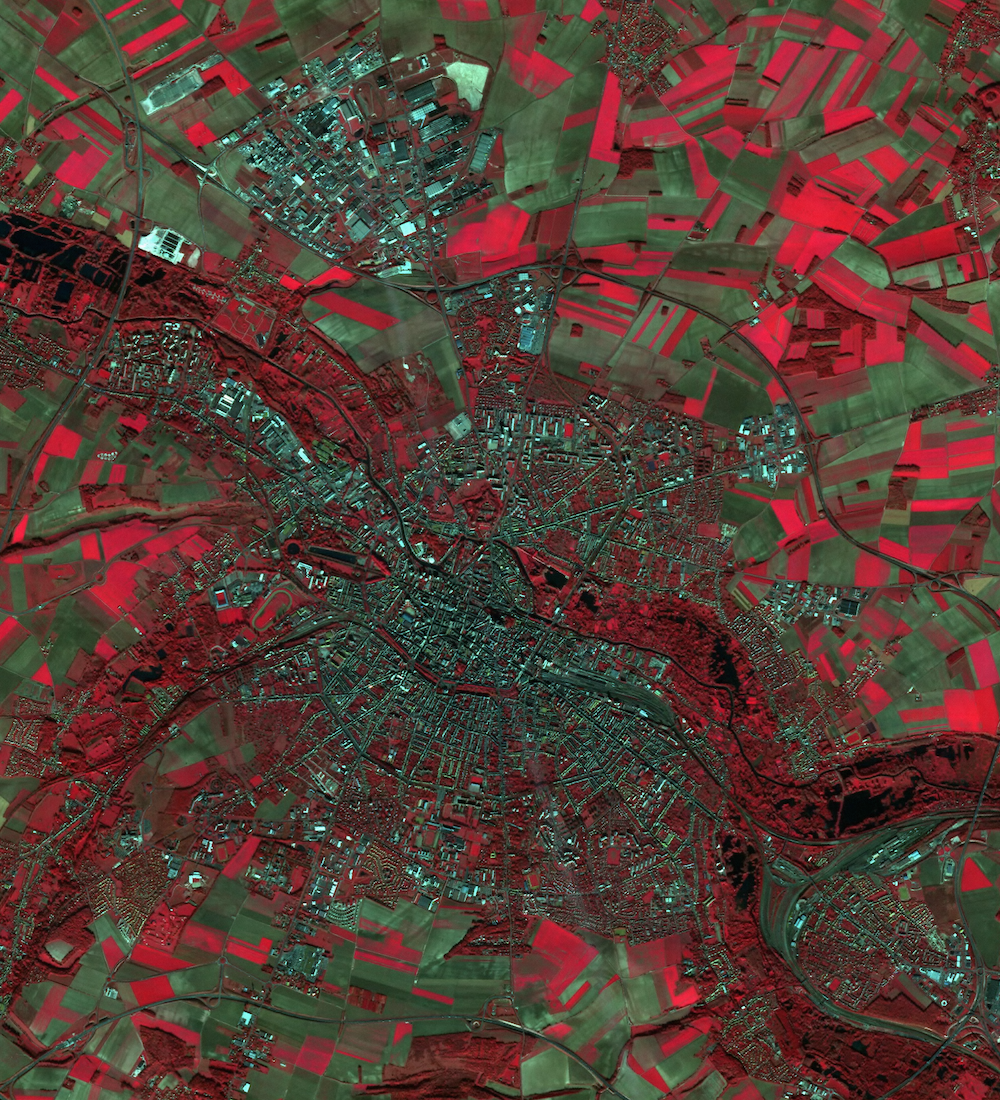
\includegraphics[scale=0.172]{Amiens_2006_SPOT_5m}}\\%pdf0.45
%         \subfigure[Mappa di \emph{training}]{
%      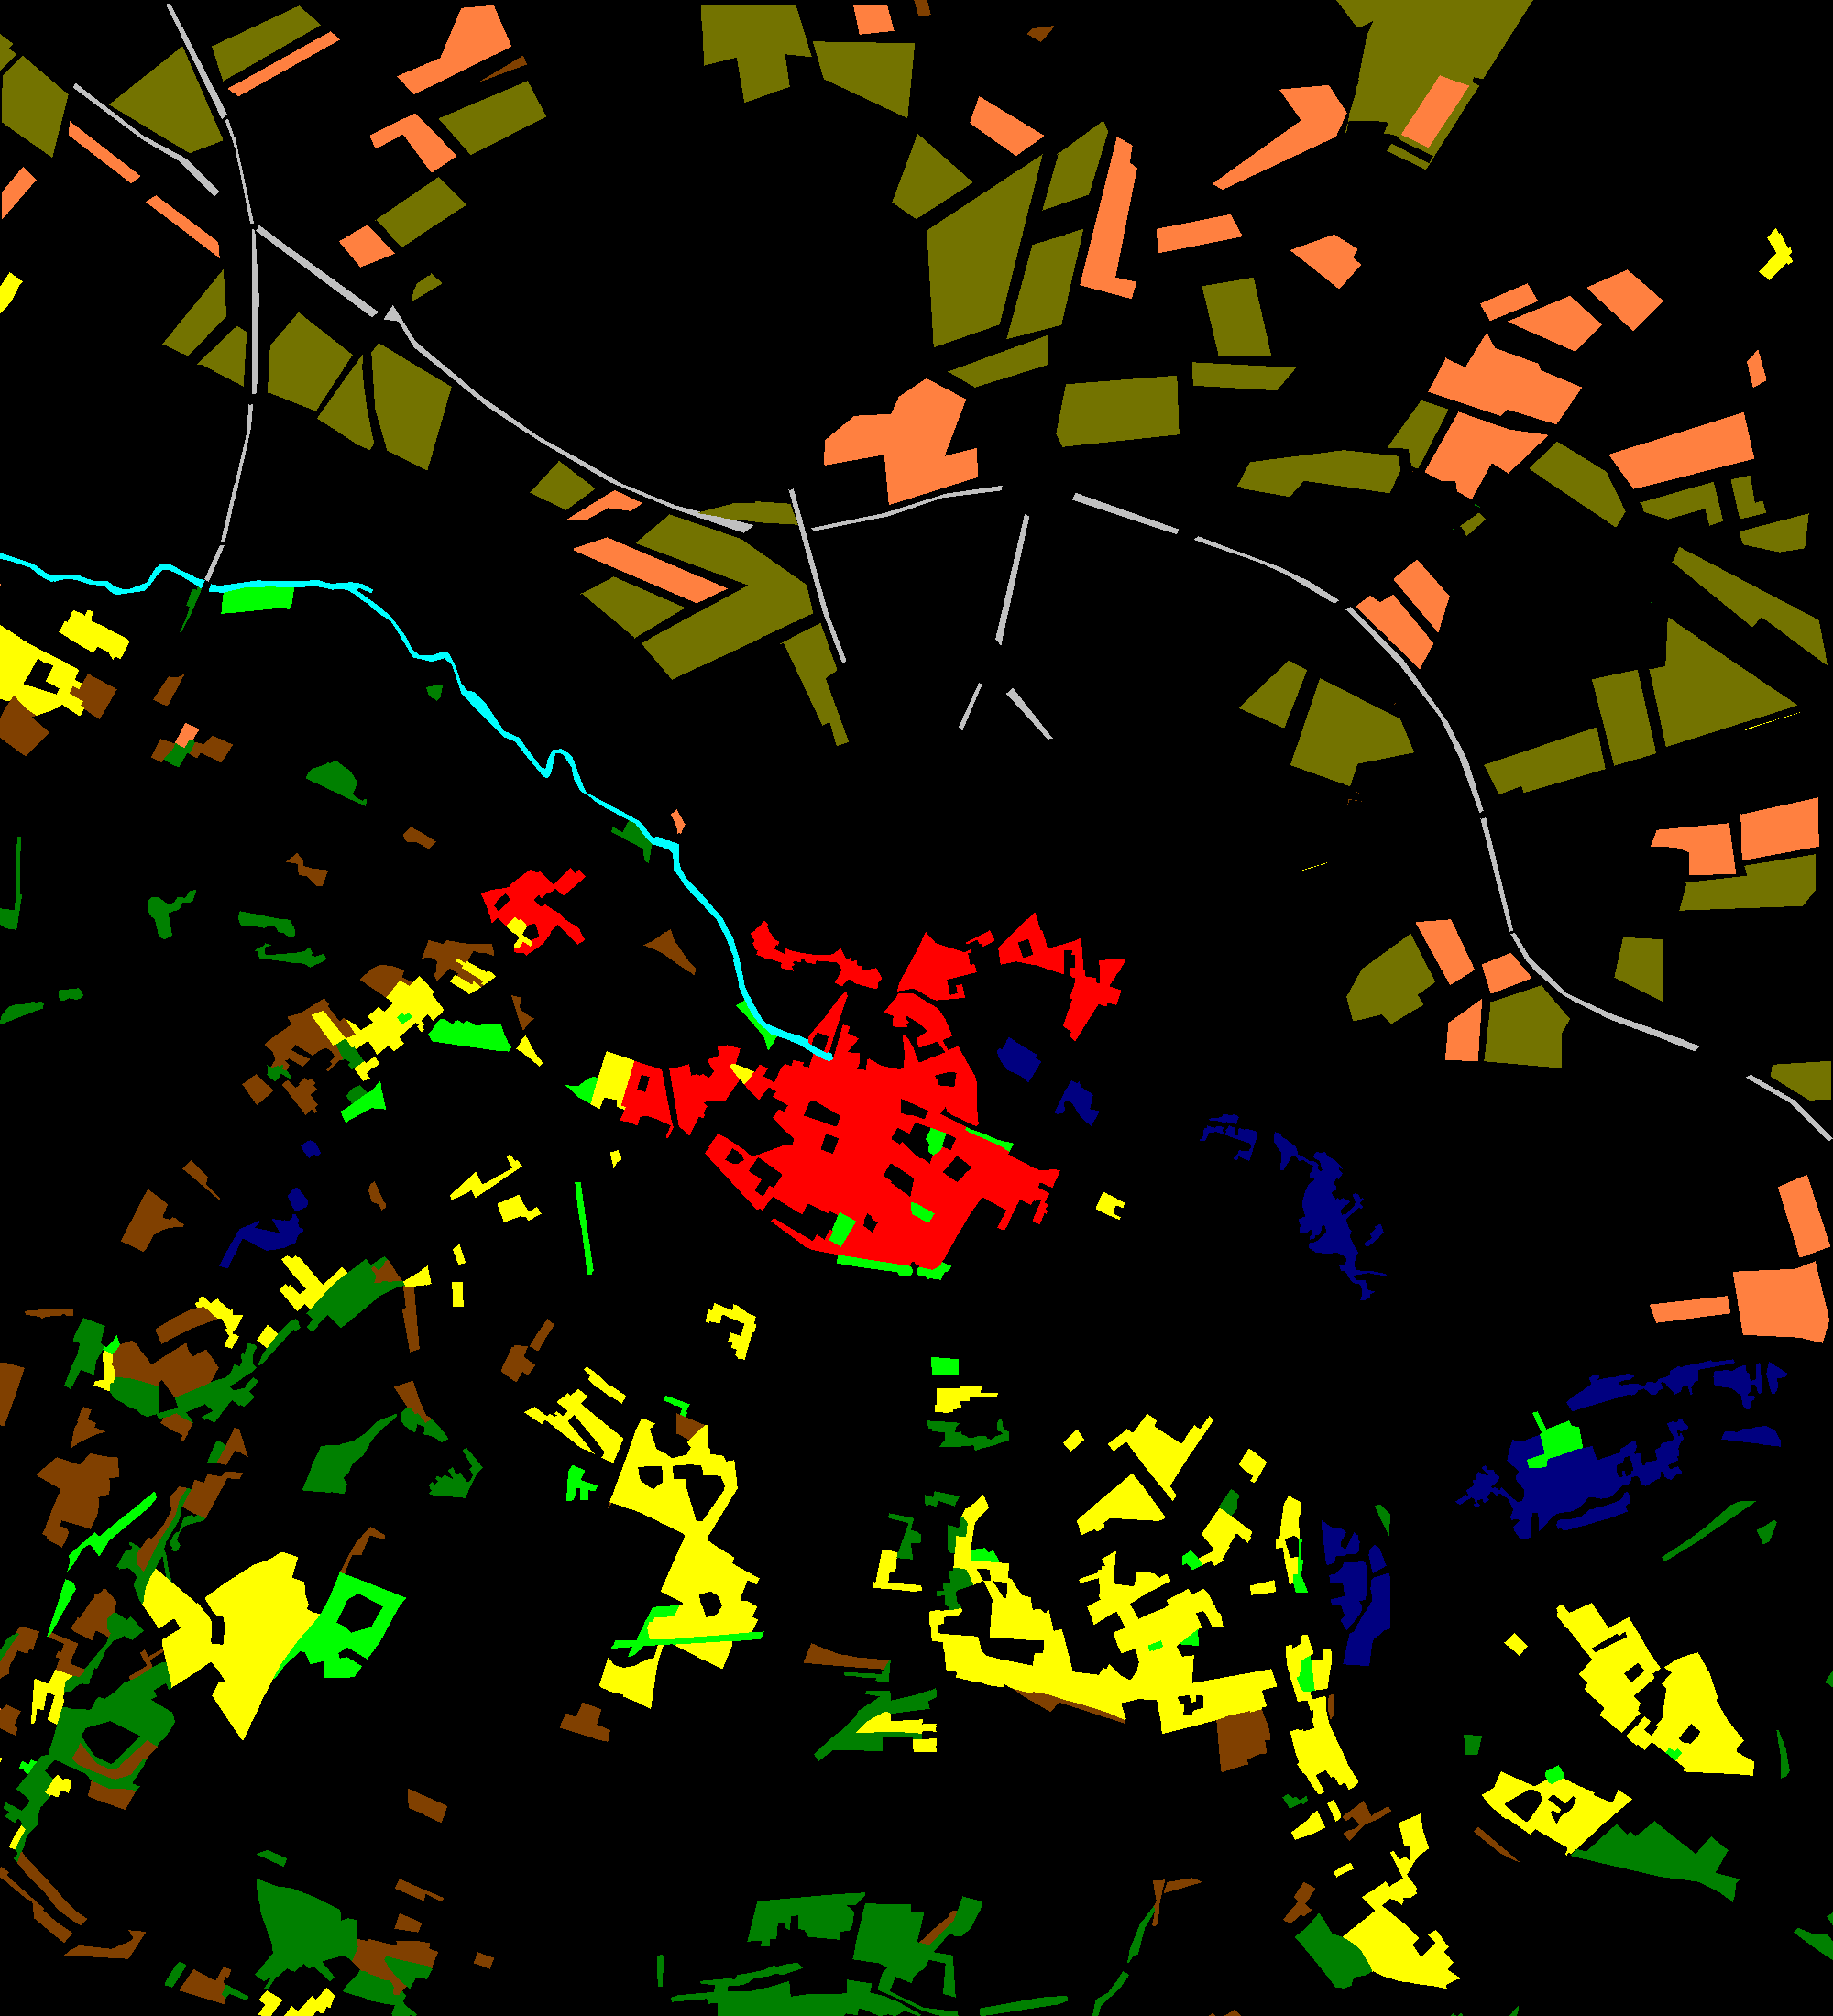
\includegraphics[scale=0.086]{GT_Amiens2006_5m_10classes_TR}}
%     \hspace{4mm}
%    \subfigure[Leggenda classi della mappa di \emph{training}]{
%      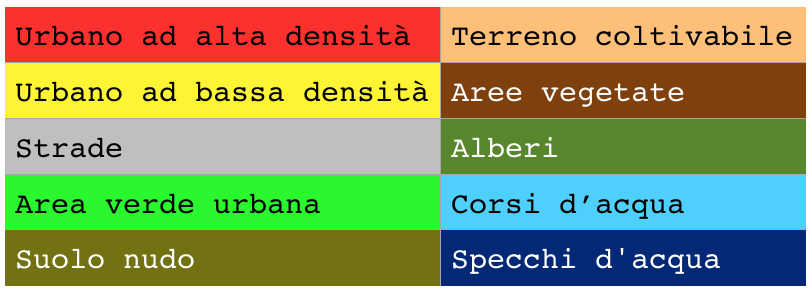
\includegraphics[scale=0.5]{Leggenda_2006_10classi}}
%    \caption{Dataset con immagine RBG in falso colore ($2000\times2200$ pixel) acquisita su Amiens (Francia) dal sensore \textsc{SPOT5 HRG}}
%    \label{fig: Amiens65m}
%  \end{figure}
%
%
%\clearpage
%\subsection{Amiens 2006 - 2.5 \textit{m}}
%L'immagine \emph{Amiens6--2.5m} è stata acquisita nel 2006 e ha risoluzione di $2.5\text{ }m/\text{pixel}$ coprendo sempre approssimativamente un'area di $10\text{ }km\times11\text{ }km$ ($4001\times4400$ pixel).\\
%L'insieme delle classi $\Omega=\left\lbrace\omega_1,\omega_2,\ldots,\omega_{7}\right\rbrace$ che costituisce il secondo \emph{dataset} è il seguente:
%\begin{enumerate}
%\item Edifici
%\item Strade e marciapiedi
%\item Aree vegetate
%\item Suolo nudo
%\item Terreno coltivabile
%\item Alberi
%\item Acqua
%\end{enumerate}
%Nella Figura \ref{fig: Amiens65m} vengono presentate le immagini caratterizzanti il primo \emph{dataset}; si osservi con attenzione la composizione dell'immagine di training: INSERIRE DISCORSO SU NUMERO DI PIXEL DI TRAINING PER CLASSI
%\clearpage
%\begin{figure}[!ht]
%   \center
%   \subfigure[Immagine telerilevata]{
%      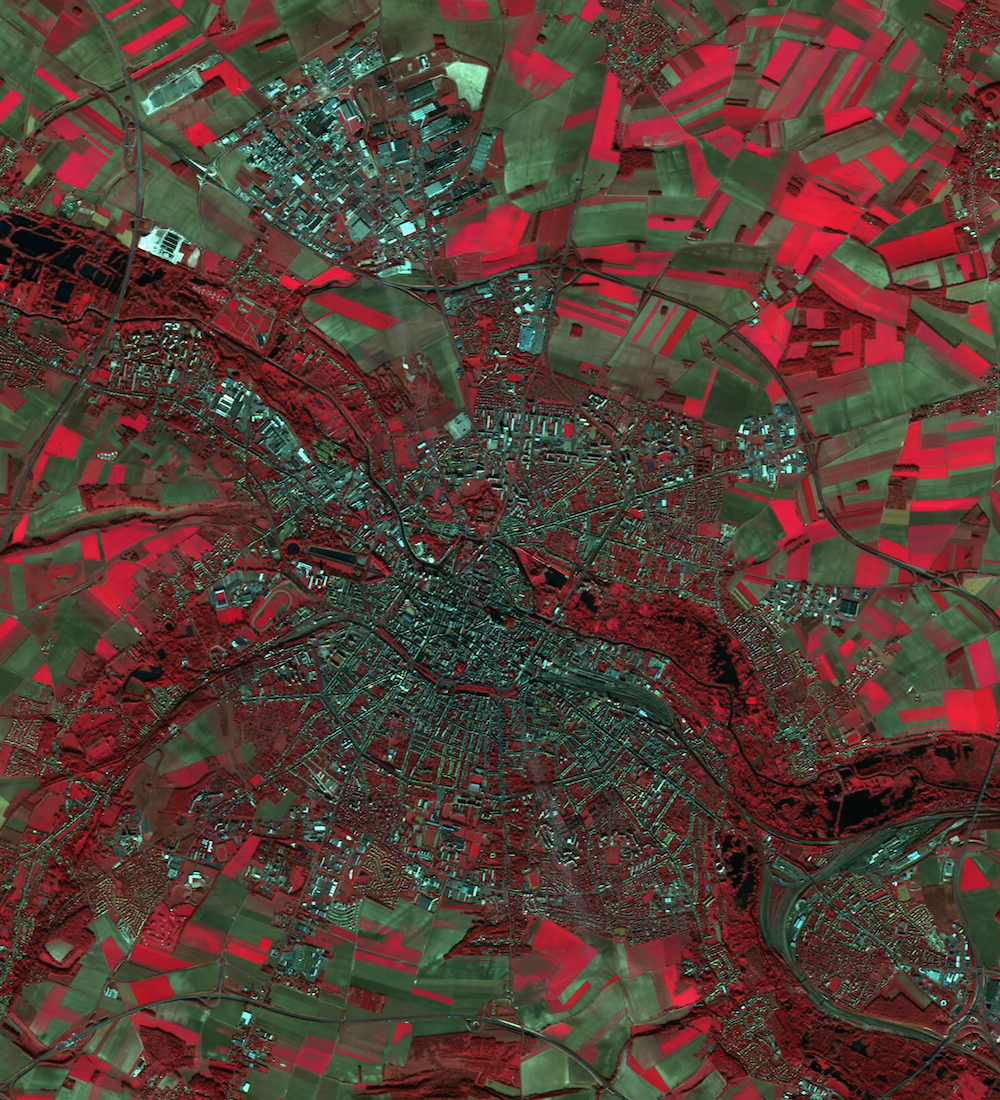
\includegraphics[scale=0.086]{Amiens_2006_SPOT_2_5m}}\\%pdf0.45
%         \subfigure[Mappa di \emph{training}]{
%      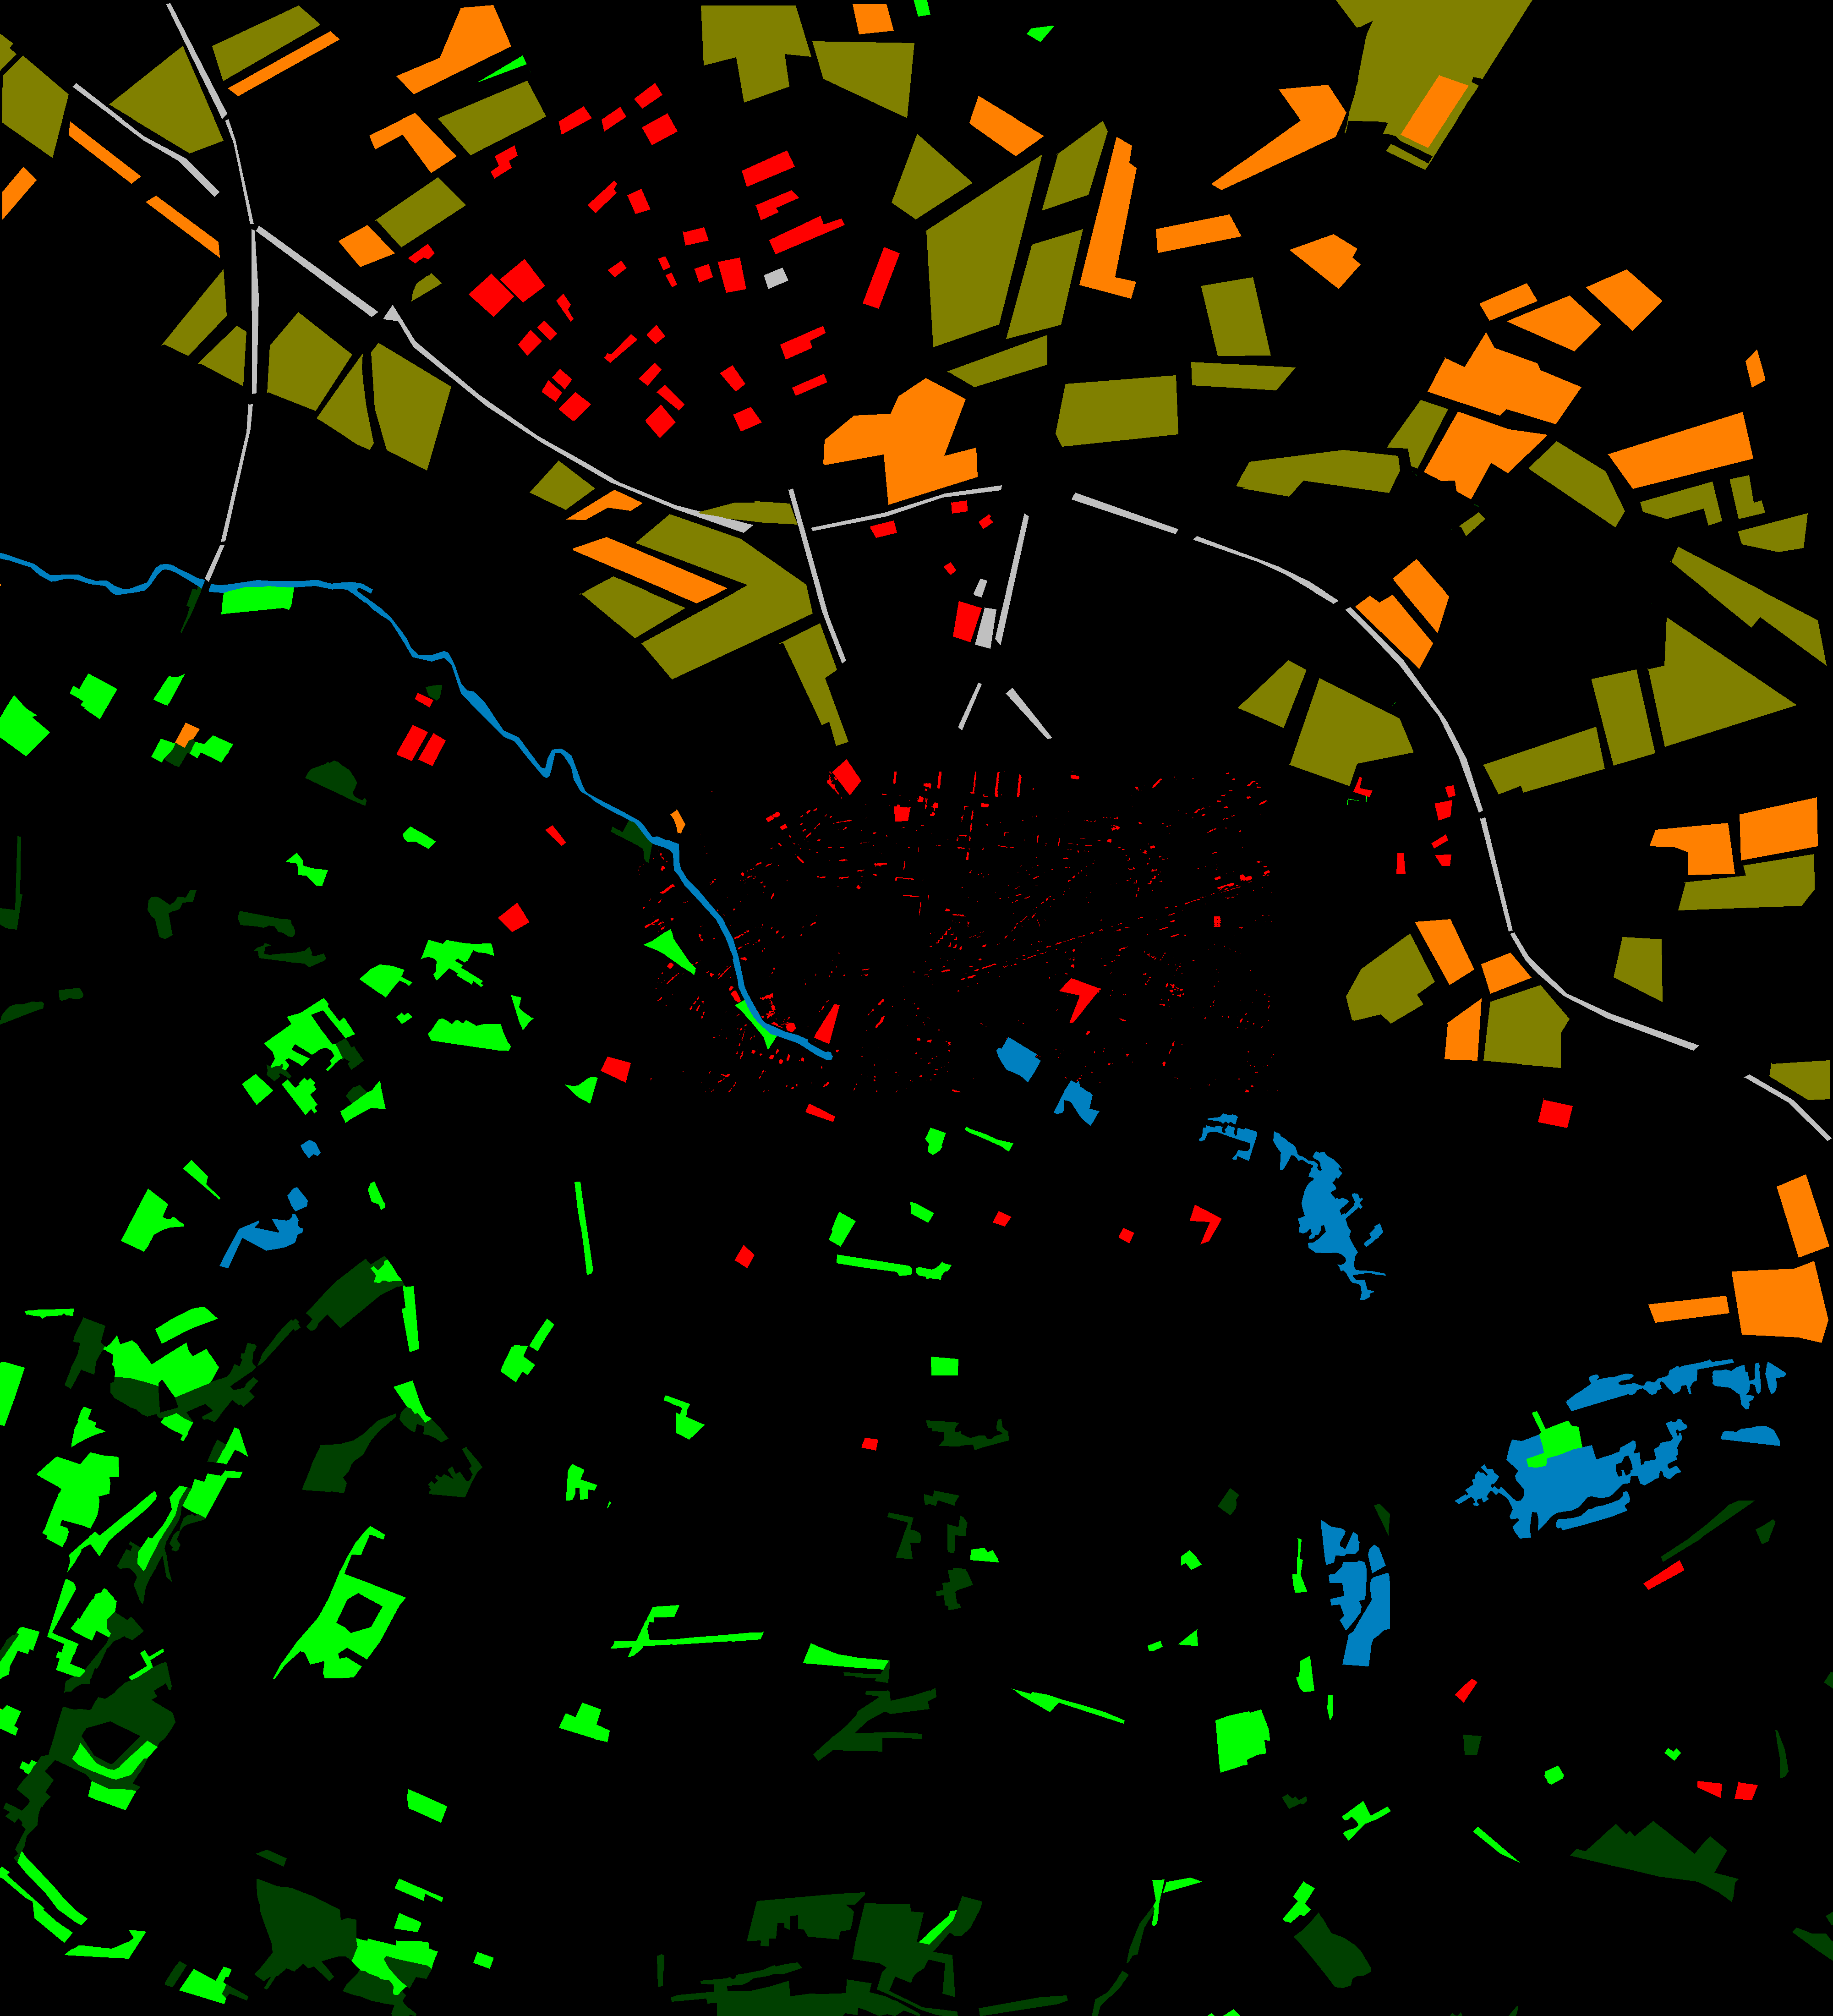
\includegraphics[scale=0.043]{GT_Amiens2006_2_5m_7classes_TR}}
%     \hspace{4mm}
%    \subfigure[Leggenda classi della mappa di \emph{training}]{
%      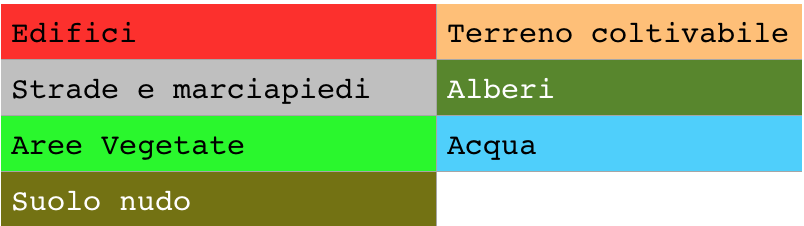
\includegraphics[scale=0.5]{Leggenda_7classi}}
%    \caption{Dataset con immagine RBG in falso colore ($2000\times2200$ pixel) acquisita su Amiens (Francia) dal sensore \textsc{SPOT5 HRG}}
%    \label{fig: Amiens65m}
%  \end{figure}
%
%
%\clearpage

%%!TEX root = ../main.tex
\chapter{Valutazione delle prestazioni del classificatore}

\label{cap:prestazioni} % Change X to a consecutive number; for referencing this chapter elsewhere, use \ref{ChapterX}

%\lhead{Capitolo \ref{prestazioni_capitolo}. \emph{Valutazione delle prestazioni del classificatore}} % Change X to a consecutive number; this is for the header on each page - perhaps a shortened title

%----------------------------------------------------------------------------------------
%	SECTION 1
%----------------------------------------------------------------------------------------


Dato un classificatore supervisionato, addestrato su un \emph{training set}, è fondamentale saper valutare l'accuratezza che può essere ottenuta quando tale classificatore è applicato a valori incogniti.\\
A tale scopo, è essenziale valutare la probabilità di errore $P_e$ del classificatore per decidere, ad esempio, se le \emph{feature} utilizzate siano sufficienti a discriminare bene le classi o se sia necessario estrarne altre (come parametri di tessitura nel caso in cui i canali spettrali non siano abbastanza discriminanti).
\clearpage

\subsection{Stima della probabilità di errore}
In presenza di $C$ classi $\omega_1,\omega_2, \ldots, \omega_C$, detta $P_i$ la probabilità di errore \emph{a priori}, la probabilità di errore $P_e$ si può esprimere nel modo seguente:
\begin{equation}
\label{eq:P_e}
P_e = P\lbrace\widehat{Y}\neq Y\rbrace= {\sum_{i=1}^C P\lbrace\widehat{Y}\neq \omega_i\vert Y = \omega_i\rbrace}P\lbrace Y =\omega_i\rbrace
\end{equation}
Dal momento che tale espressione è calcolabile solo in pochissimi casi semplici, per valutarla si adotta generalmente un approccio empirico, che stima la $P_e$ come la percentuale dei pixel di test classificati erroneamente.\\
Solitamente la $P_e$ viene valutata su un insieme di campioni pre-etichettati(\emph{test set}) diverso rispetto a quello utilizzato per addestrare il classificatore(\emph{training set}). Questa tecnica, detta \emph{hold-out}, permette una misura delle prestazioni priva di \emph{bias} in quanto eseguita su istanze non utilizzate in fase di apprendimento.\\
Per evitare il fenomeno dell'\emph{overfitting},\footnote{Si parla di \emph{overfitting} quando la funzione discriminante è strettamente dipendente dai campioni di \emph{training} specifici utilizzati per calcolarla ed è quindi particolarmente inefficace quando applicata a campioni incogniti} un'ipotesi fondamentale per stimare $P_e$ come frequenza relativa degli errori sul \emph{test set} è che i campioni pre-etichettati siano indipendenti e identicamente distribuiti (i.i.d). Per questa ragione, è buona norma prelevare i campioni di \emph{training} e di \emph{test} in regioni dell'immagine spazialmente disgiunte tra loro.\\
E' altrettanto importante effettuare un'analisi qualitativa dell'intera mappa, mediante foto-interpretazione, come complemento alla valutazione quantitativa delle prestazioni di classificazione sui campioni di test.

\subsection{Matrice di confusione e parametri di accuratezza}
La $P_e$ fornisce una valutazione complessiva delle prestazioni del classificatore, senza però differenziare gli errori commessi in corrispondenza di classi diverse. Per una valutazione più dettagliata la matrice di confusione (\emph{confusion matrix}) è la tipologia di osservazione statistica maggiormente utilizzata: il risultato della classificazione sulle aree campione viene confrontato con la verità al suolo [Congalton]. Questa è una matrice $C \times C$, il cui elemento $e_{ij}$ è il numero di pixel di test della classe $\omega_i$ che il classificatore ha assegnato alla classe $\omega_j$. Sulla diagonale $i=j$ della matrice di confusione si leggono dunque i numeri di pixel di test classificati in modo corretto. Questo tipo di analisi statistica consente non solo di quantificare il successo ottenuto dalla procedura, ma anche di focalizzare i punti critici del processo di classificazione, ovvero le classi meno distinguibili tra loro. \\
L'accuratezza della classificazione può essere valutata con diversi parametri numerici, tra cui i più utilizzati sono:
\begin{itemize}
\item L' \emph{average accuracy} (AA) delle C classi è la media rispetto al numero di classi delle frazioni di pixel correttamente classificati (classe per classe), ed è data da:
\begin{equation}
\label{eq:AA}
AA=\dfrac{1}{C}\sum_{i=1}^C\dfrac{e_{ij}}{\sum_{j=1}^C e_{ij}}
\end{equation}
\item L'\emph{overall accuracy }(OA) è la percentuale di pixel classificati correttamente sull'intero test set ed è data da:
\begin{equation}
\label{eq:OA}
OA= \dfrac{1}{t}\sum_{i=1}^C e_{ij}
\end{equation}
\item Il parametro "$\kappa$", rappresenta una modifica dell' OA finalizzata a tenere conto in modo più completo della distribuzione degli errori tra le diverse classi, ed è dato da:
\begin{equation}
\label{eq:K}
\kappa=\dfrac{OA-\frac{1}{t^2}\sum_{i=1}^C\sum_{j=1}^C\sum_{k=1}^C e_{ij}e_{ki}}{1-\frac{1}{t^2}\sum_{i=1}^C\sum_{j=1}^C\sum_{k=1}^C e_{ij} e_{ki}}
\end{equation}
dove t è il numero di pixel di test.
\end{itemize}


\chapter{Risultati sperimentali} % Main chapter title

\label{cap:risultati} % Change X to a consecutive number; for referencing this chapter elsewhere, use \ref{ChapterX}

%\lhead{Capitolo \ref{chapter_Risultati_sperimentali}. \emph{Risultati sperimentali}} % Change X to a consecutive number; this is for the header on each page - perhaps a shortened title


In questo capitolo verranno presentati tre casi di studio e verrà fatta un analisi delle variazioni di prestazioni al variare dei parametri dell’algoritmo  HOG, evidenziando i valori ottimali. 
Successivamente verranno presentati i risultati ottenuti valutando anche i punti in cui questo algoritmo non ha dato risultati soddisfacenti, cercando di esporre le cause che hanno generato questi errori.

\clearpage

\section{Descrizione dei \emph{dataset}}
In questa tesi sono stati analizzati tre casi rilevanti, tutti relativi alla classificazione dell'area urbana di Amiens (Francia).  Si tratta di un problema di classificazione interessante in quanto le regioni coinvolte sono caratterizzate da aree omogenee (come corsi d'acqua), strutture geometriche ben definite (come edifici e strade) e zone di suolo con\emph{ pattern} regolari (come campi coltivabili e non).\\
Il \emph{dataset} per ogni esperimento è costituito dall'immagine telerilevata, dalla mappa di \emph{training} e dalla mappa di \emph{testing}.
Le immagini telerilevate sono state acquisite dal sensore passivo \textsc{SPOT5 HRG} con risoluzione spettrale a tre canali, corrispondenti alle lunghezze d'onda del verde (G, $495–570\text{ } nm$), del rosso (R, $620–750\text{ } nm$) e dell'infrarosso (NIR, \emph{Near InfraRed} $0.75–1.4\text{ } \mu m$).
 

\subsection{Amiens 2006 - 5 \textit{m}}
L'immagine \emph{Amiens6--5m} è stata acquisita nel 2006 e ha risoluzione di $5\text{ }m/\text{pixel}$, coprendo approssimativamente un'area di $10\text{ }km\times11\text{ }km$ ($2000\times2200$ pixel).\\
L'insieme delle classi $\Omega=\left\lbrace\omega_1,\omega_2,\ldots,\omega_{10}\right\rbrace$ che costituisce questo primo esperimento è il seguente:
\begin{enumerate}
\item Area urbana ad alta densità
\item Area urbana a bassa densità
\item Strade
\item Area verde urbana 
\item Suolo nudo
\item Terreno coltivabile
\item Terreno non coltivabile 
\item Alberi
\item Corsi d'acqua
\item Bacini idrografici
\end{enumerate}
Nella Figura \ref{fig: Amiens65m} vengono presentate le immagini caratterizzanti il primo \emph{dataset}; si osservi con attenzione la composizione dell'immagine di \emph{training}: 
\\INSERIRE DISCORSO SU NUMERO DI PIXEL DI TRAINING PER CLASSI

\clearpage
\begin{figure}[!ht]
   \center
   \subfigure[Immagine telerilevata]{
      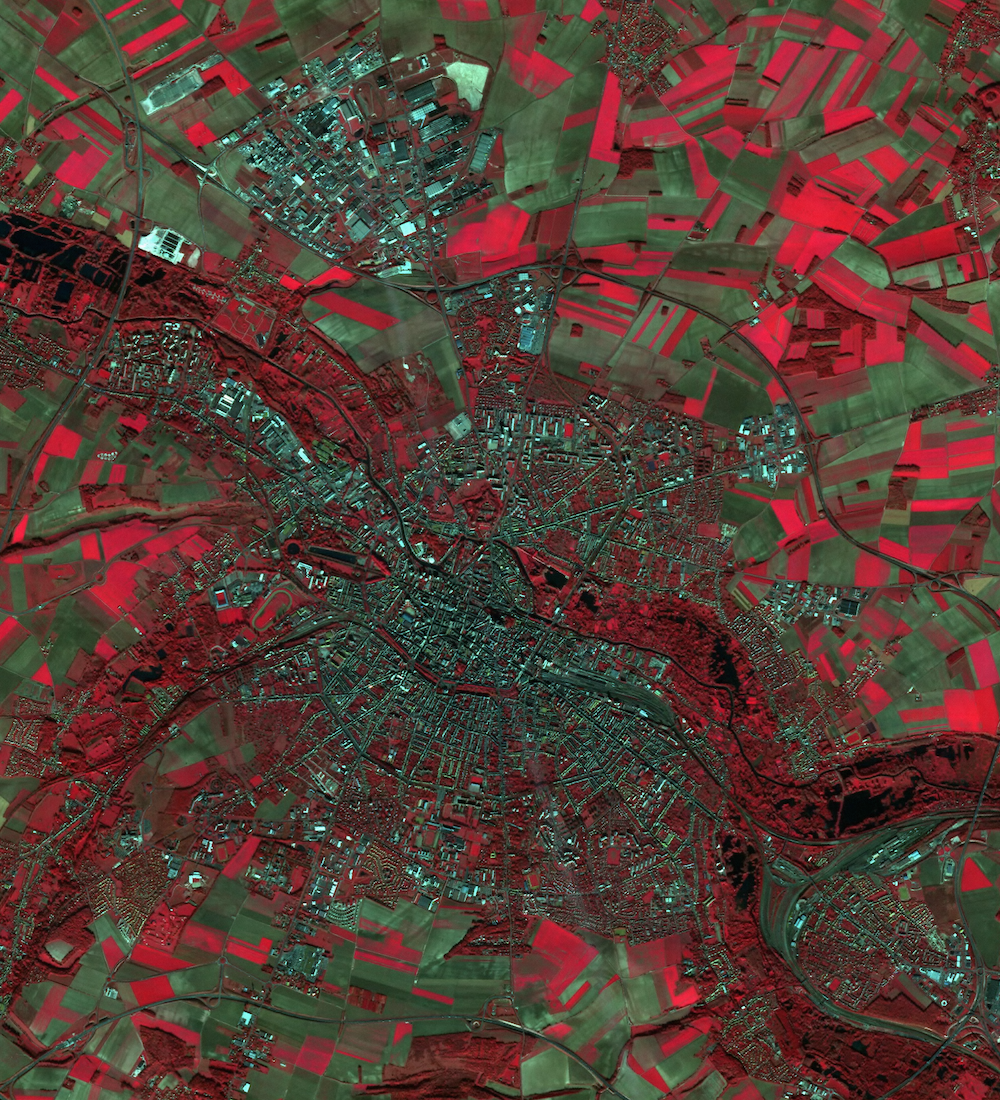
\includegraphics[width=0.8\textwidth]{Amiens_2006_SPOT_5m}}\\%pdf0.45
         \subfigure[Mappa di \emph{training}]{
      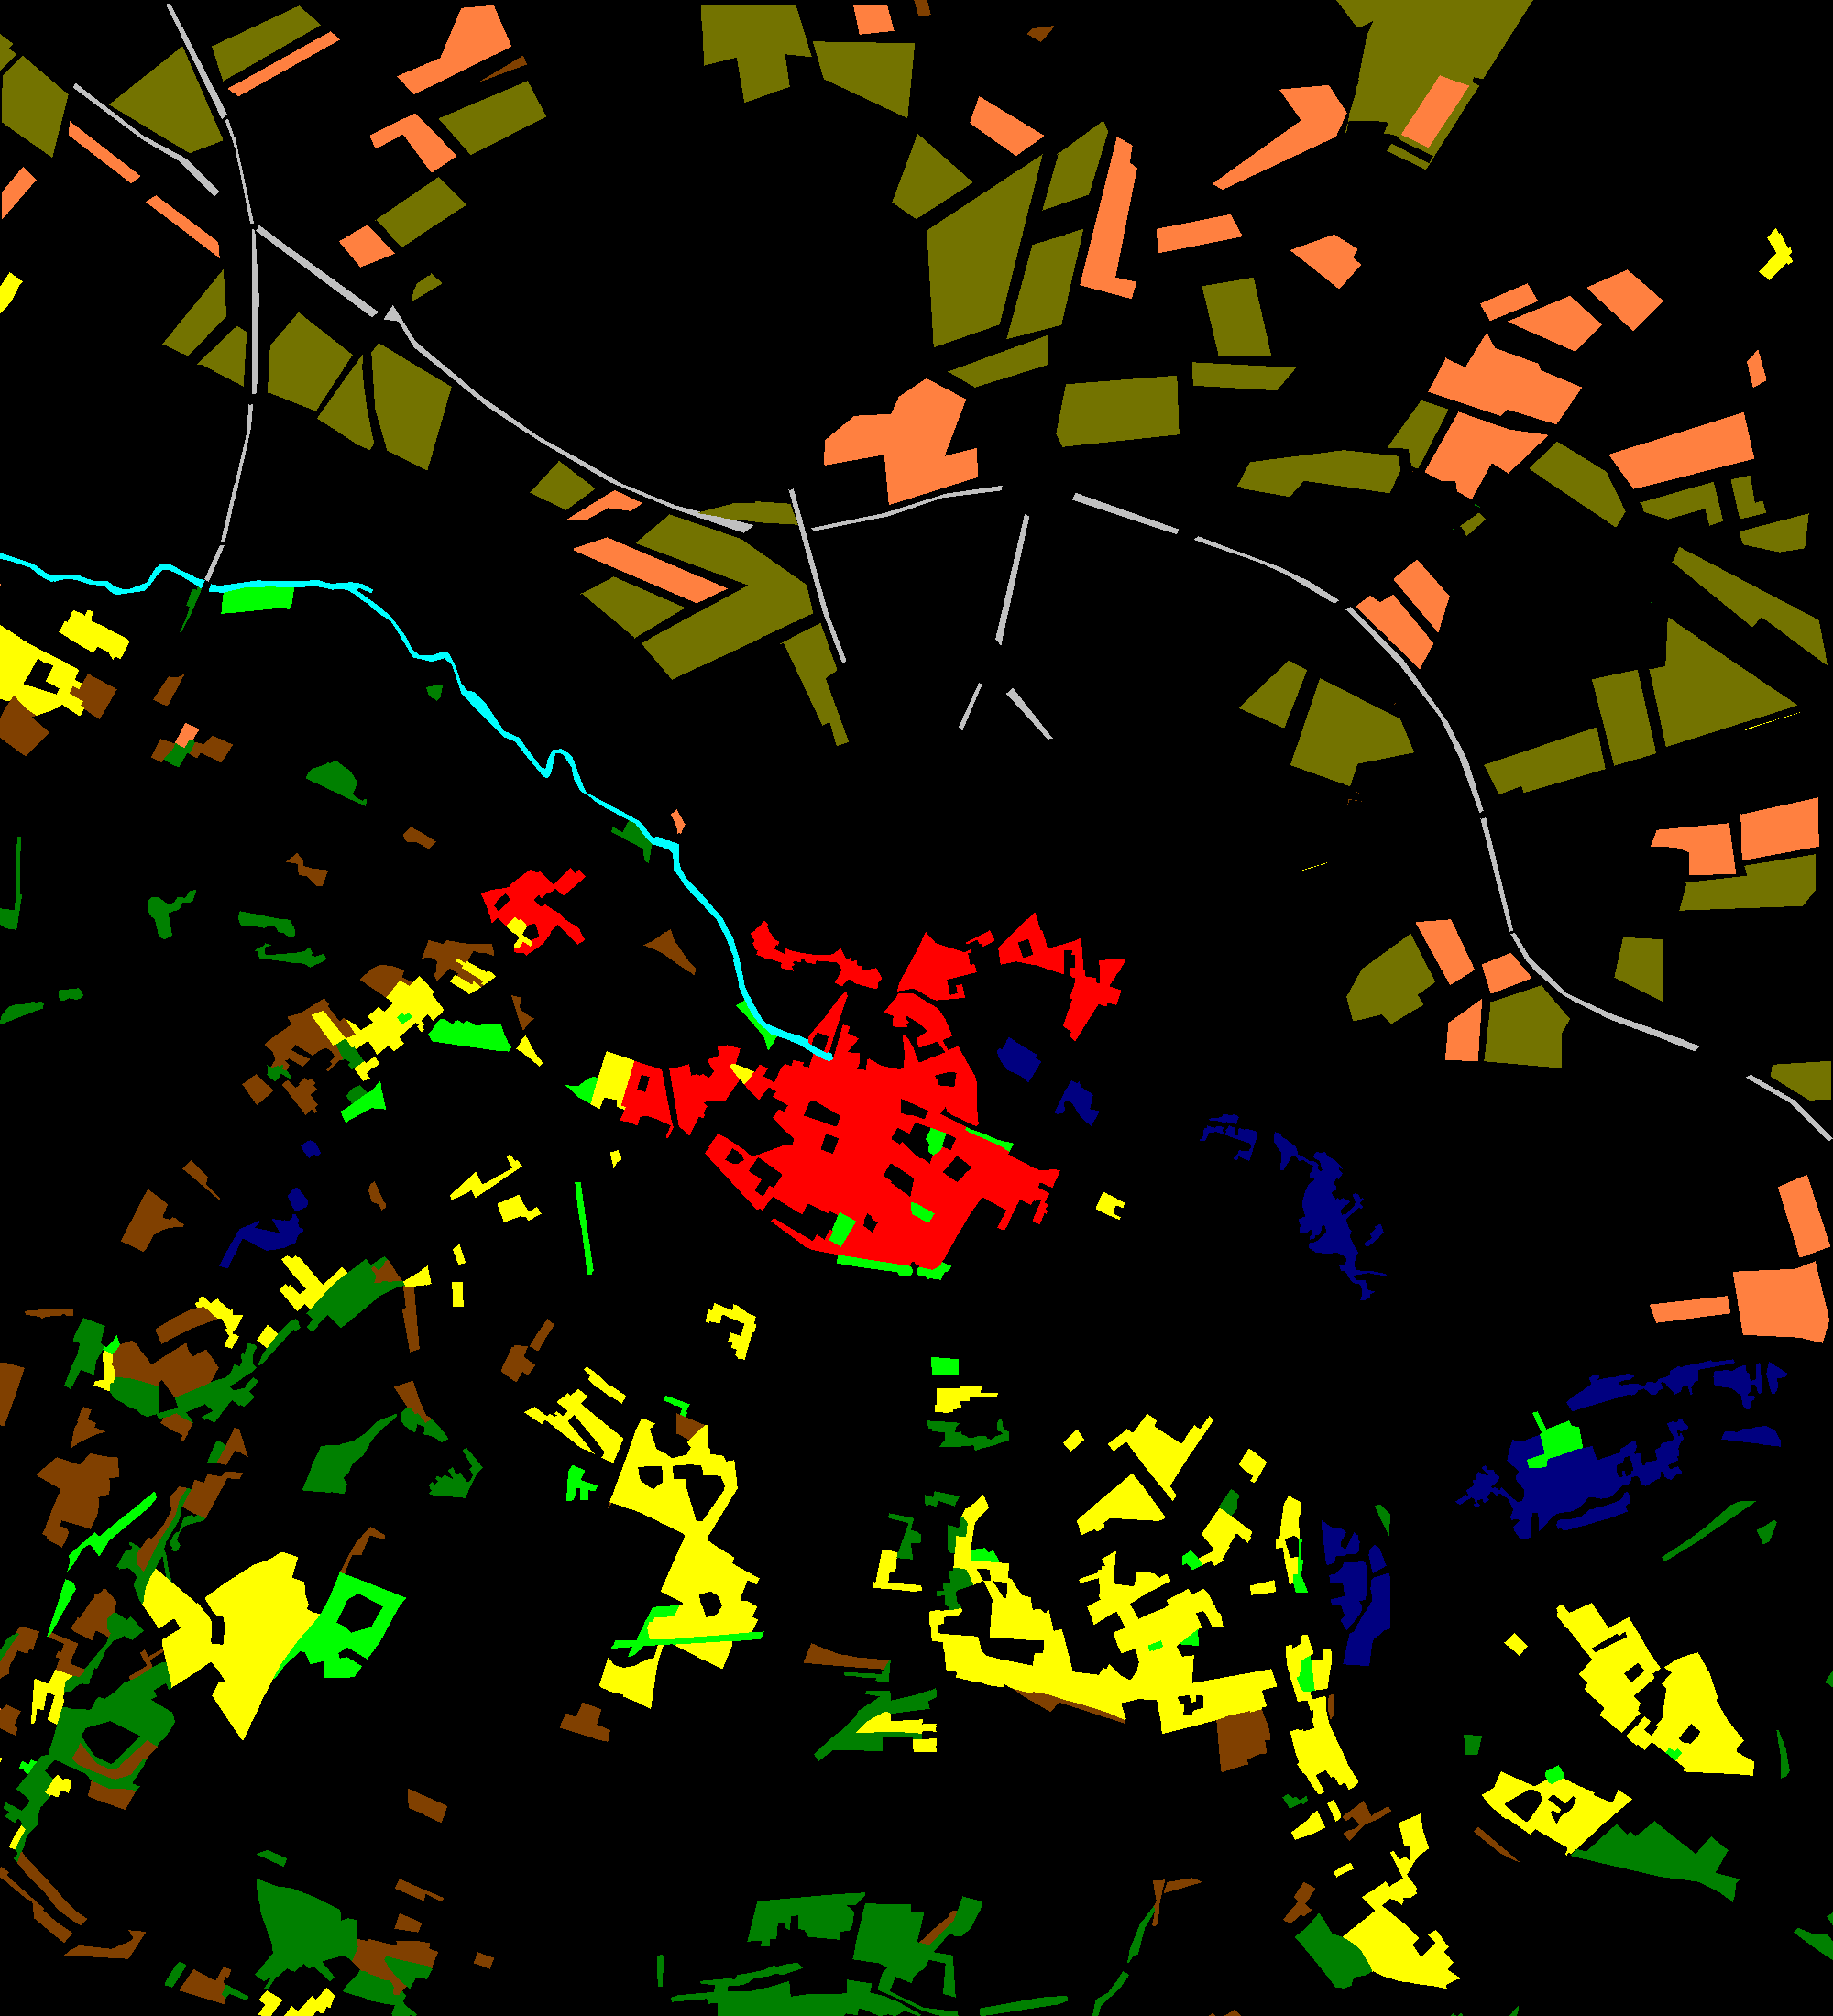
\includegraphics[width=0.4\textwidth]{GT_Amiens2006_5m_10classes_TR}}
     \hspace{4mm}
    \subfigure[Legenda classi della mappa di \emph{training}]{
      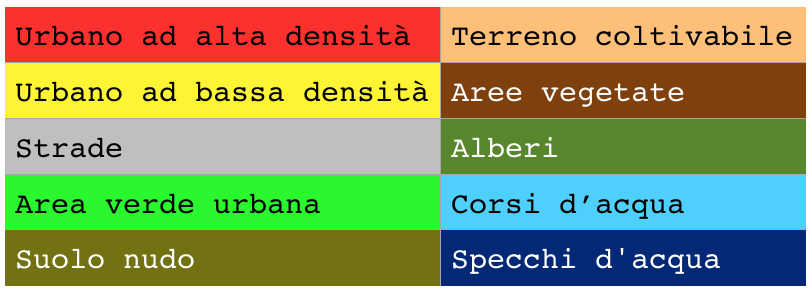
\includegraphics[scale=0.5]{Leggenda_2006_10classi}}
    \caption{\emph{Dataset} con immagine RBG in falso colore ($2000\times2200$ pixel) acquisita su Amiens (Francia) dal sensore \textsc{SPOT5 HRG}}
    \label{fig: Amiens65m}
  \end{figure}
  
\clearpage
\subsection{Amiens 2006 - 2.5 \textit{m}}
L'immagine \emph{Amiens6--2.5m} è stata acquisita sempre nel 2006, ma ha una risoluzione  spaziale maggiore del caso precedente di $2.5\text{ }m/\text{pixel}$  e copre sempre approssimativamente un'area di $10\text{ }km\times11\text{ }km$ ($4001\times4400$ pixel).\\
L'insieme delle classi $\Omega=\left\lbrace\omega_1,\omega_2,\ldots,\omega_{7}\right\rbrace$ che costituisce il secondo \emph{dataset} è il seguente:
\begin{enumerate}
\item Edifici
\item Strade e marciapiedi
\item Aree vegetate
\item Suolo nudo
\item Terreno coltivabile
\item Alberi
\item Acqua
\end{enumerate}
Nella Figura \ref{fig: Amiens62_5m} vengono presentate le immagini caratterizzanti il primo \emph{dataset}; si osservi con attenzione la composizione dell'immagine di \emph{training}: INSERIRE DISCORSO SU NUMERO DI PIXEL DI TRAINING PER CLASSI
\clearpage
\begin{figure}[!ht]
   \center
   \subfigure[Immagine telerilevata]{
      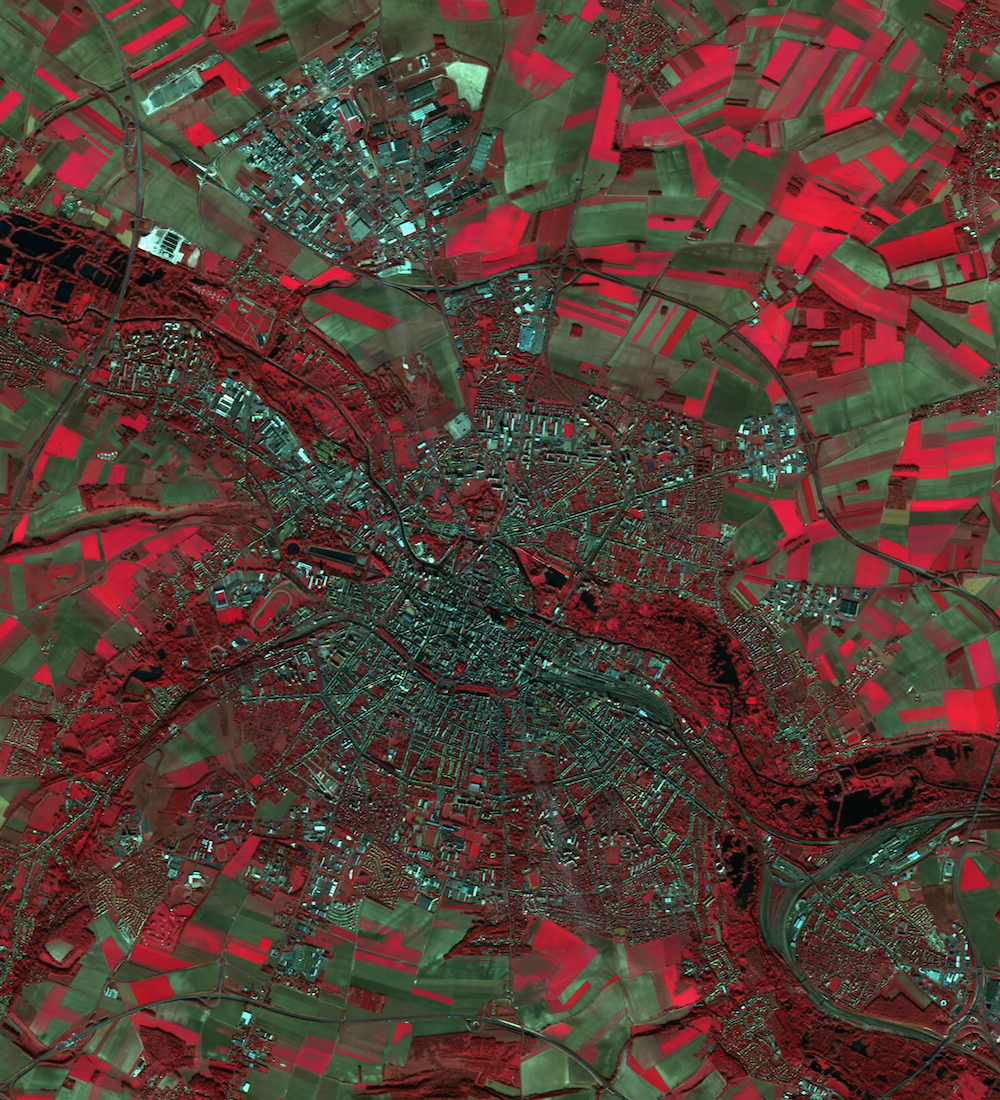
\includegraphics[width=0.8\textwidth]{Amiens_2006_SPOT_2_5m}}\\%pdf0.45
         \subfigure[Mappa di \emph{training}]{
      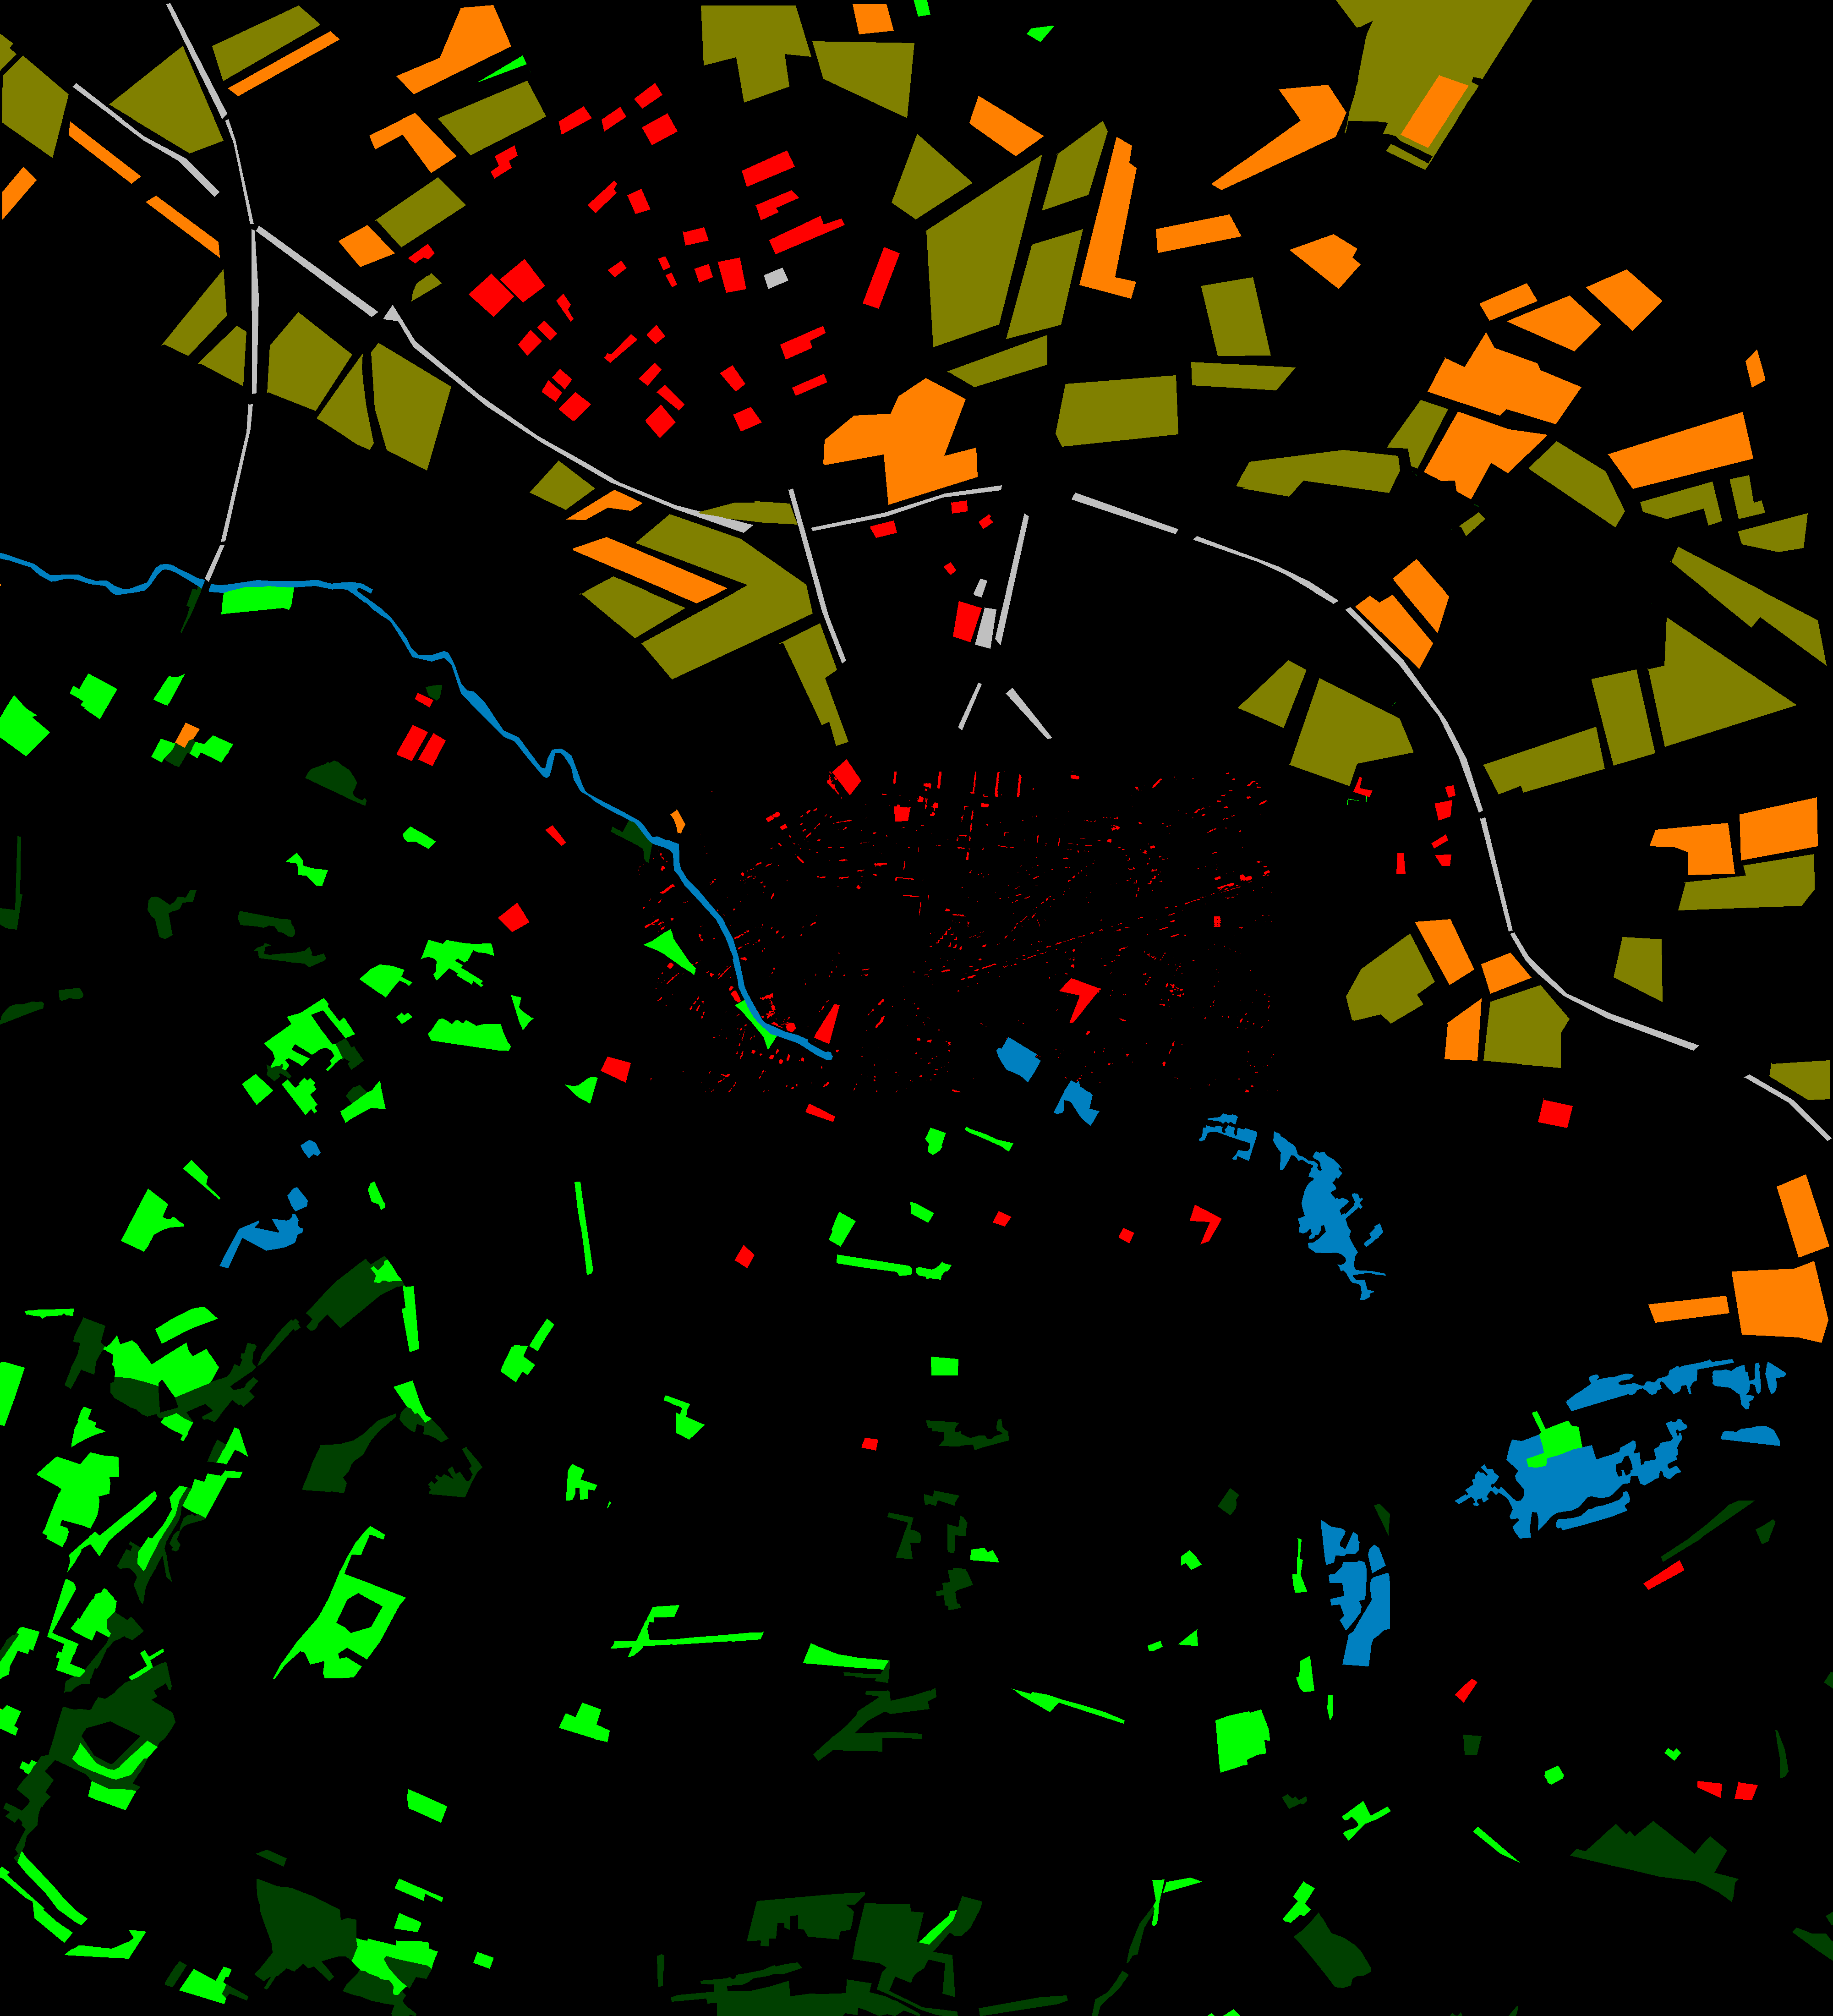
\includegraphics[width=0.4\textwidth]{GT_Amiens2006_2_5m_7classes_TR}}
     \hspace{4mm}
    \subfigure[Legenda classi della mappa di \emph{training}]{
      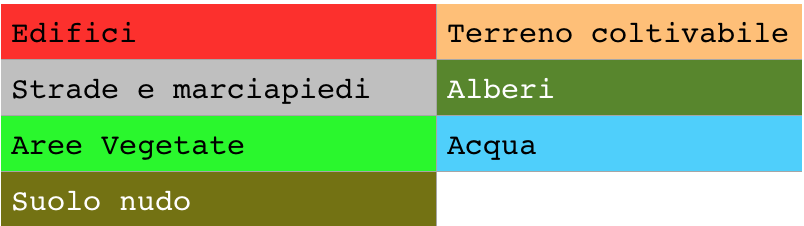
\includegraphics[scale=0.5]{Leggenda_7classi}}
    \caption{\emph{Dataset} con immagine RBG in falso colore ($4000\times4400$ pixel) acquisita su Amiens (Francia) dal sensore \textsc{SPOT5 HRG} nel 2006}
    \label{fig: Amiens62_5m}
  \end{figure}
\clearpage


\subsection{Amiens 2012 - 2.5 \textit{m}}
L'immagine \emph{Amiens12--2.5m} è stata acquisita nel 2012 ed ha  risoluzione spaziale di $2.5\text{ }m/\text{pixel}$, coprendo sempre un'area di circa $10\text{ }km\times11\text{ }km$ ($4001\times4400$ pixel).\\
L'insieme delle classi $\Omega=\left\lbrace\omega_1,\omega_2,\ldots,\omega_{7}\right\rbrace$, che costituisce il \emph{dataset}, è lo stesso del precedente. Per uniformità vengono ugualmente riportate:
\begin{enumerate}
\item Edifici
\item Strade e marciapiedi
\item Aree vegetate
\item Suolo nudo
\item Terreno coltivabile
\item Alberi
\item Acqua
\end{enumerate}
Nella Figura \ref{fig: Amiens122_5m} vengono presentate le immagini caratterizzanti il primo \emph{dataset}; si osservi con attenzione la composizione dell'immagine di \emph{training}.
\clearpage
\begin{figure}[!ht]
   \center
   \subfigure[Immagine telerilevata]{
      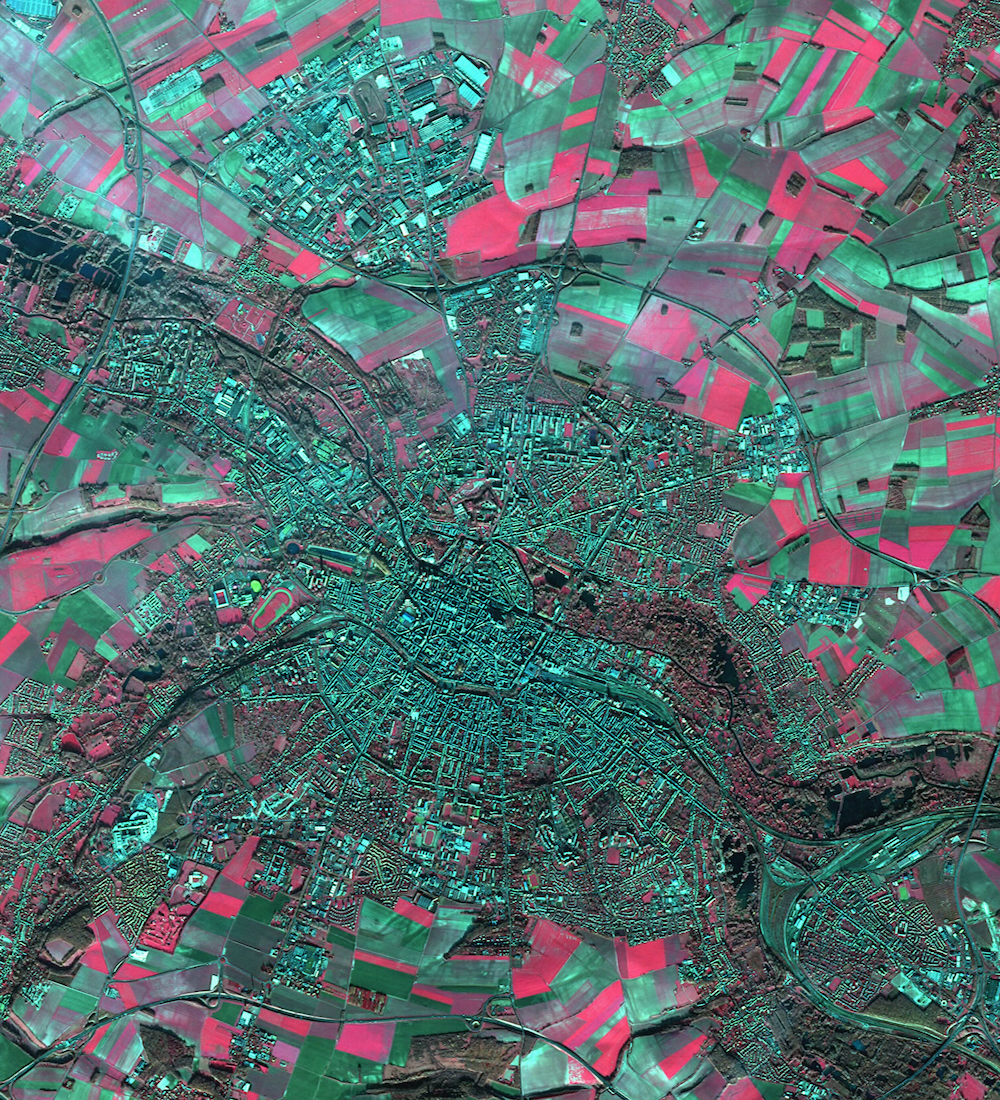
\includegraphics[width=0.8\textwidth]{Amiens_2012_SPOT_2_5m}}\\%pdf0.45
         \subfigure[Mappa di \emph{training}]{
      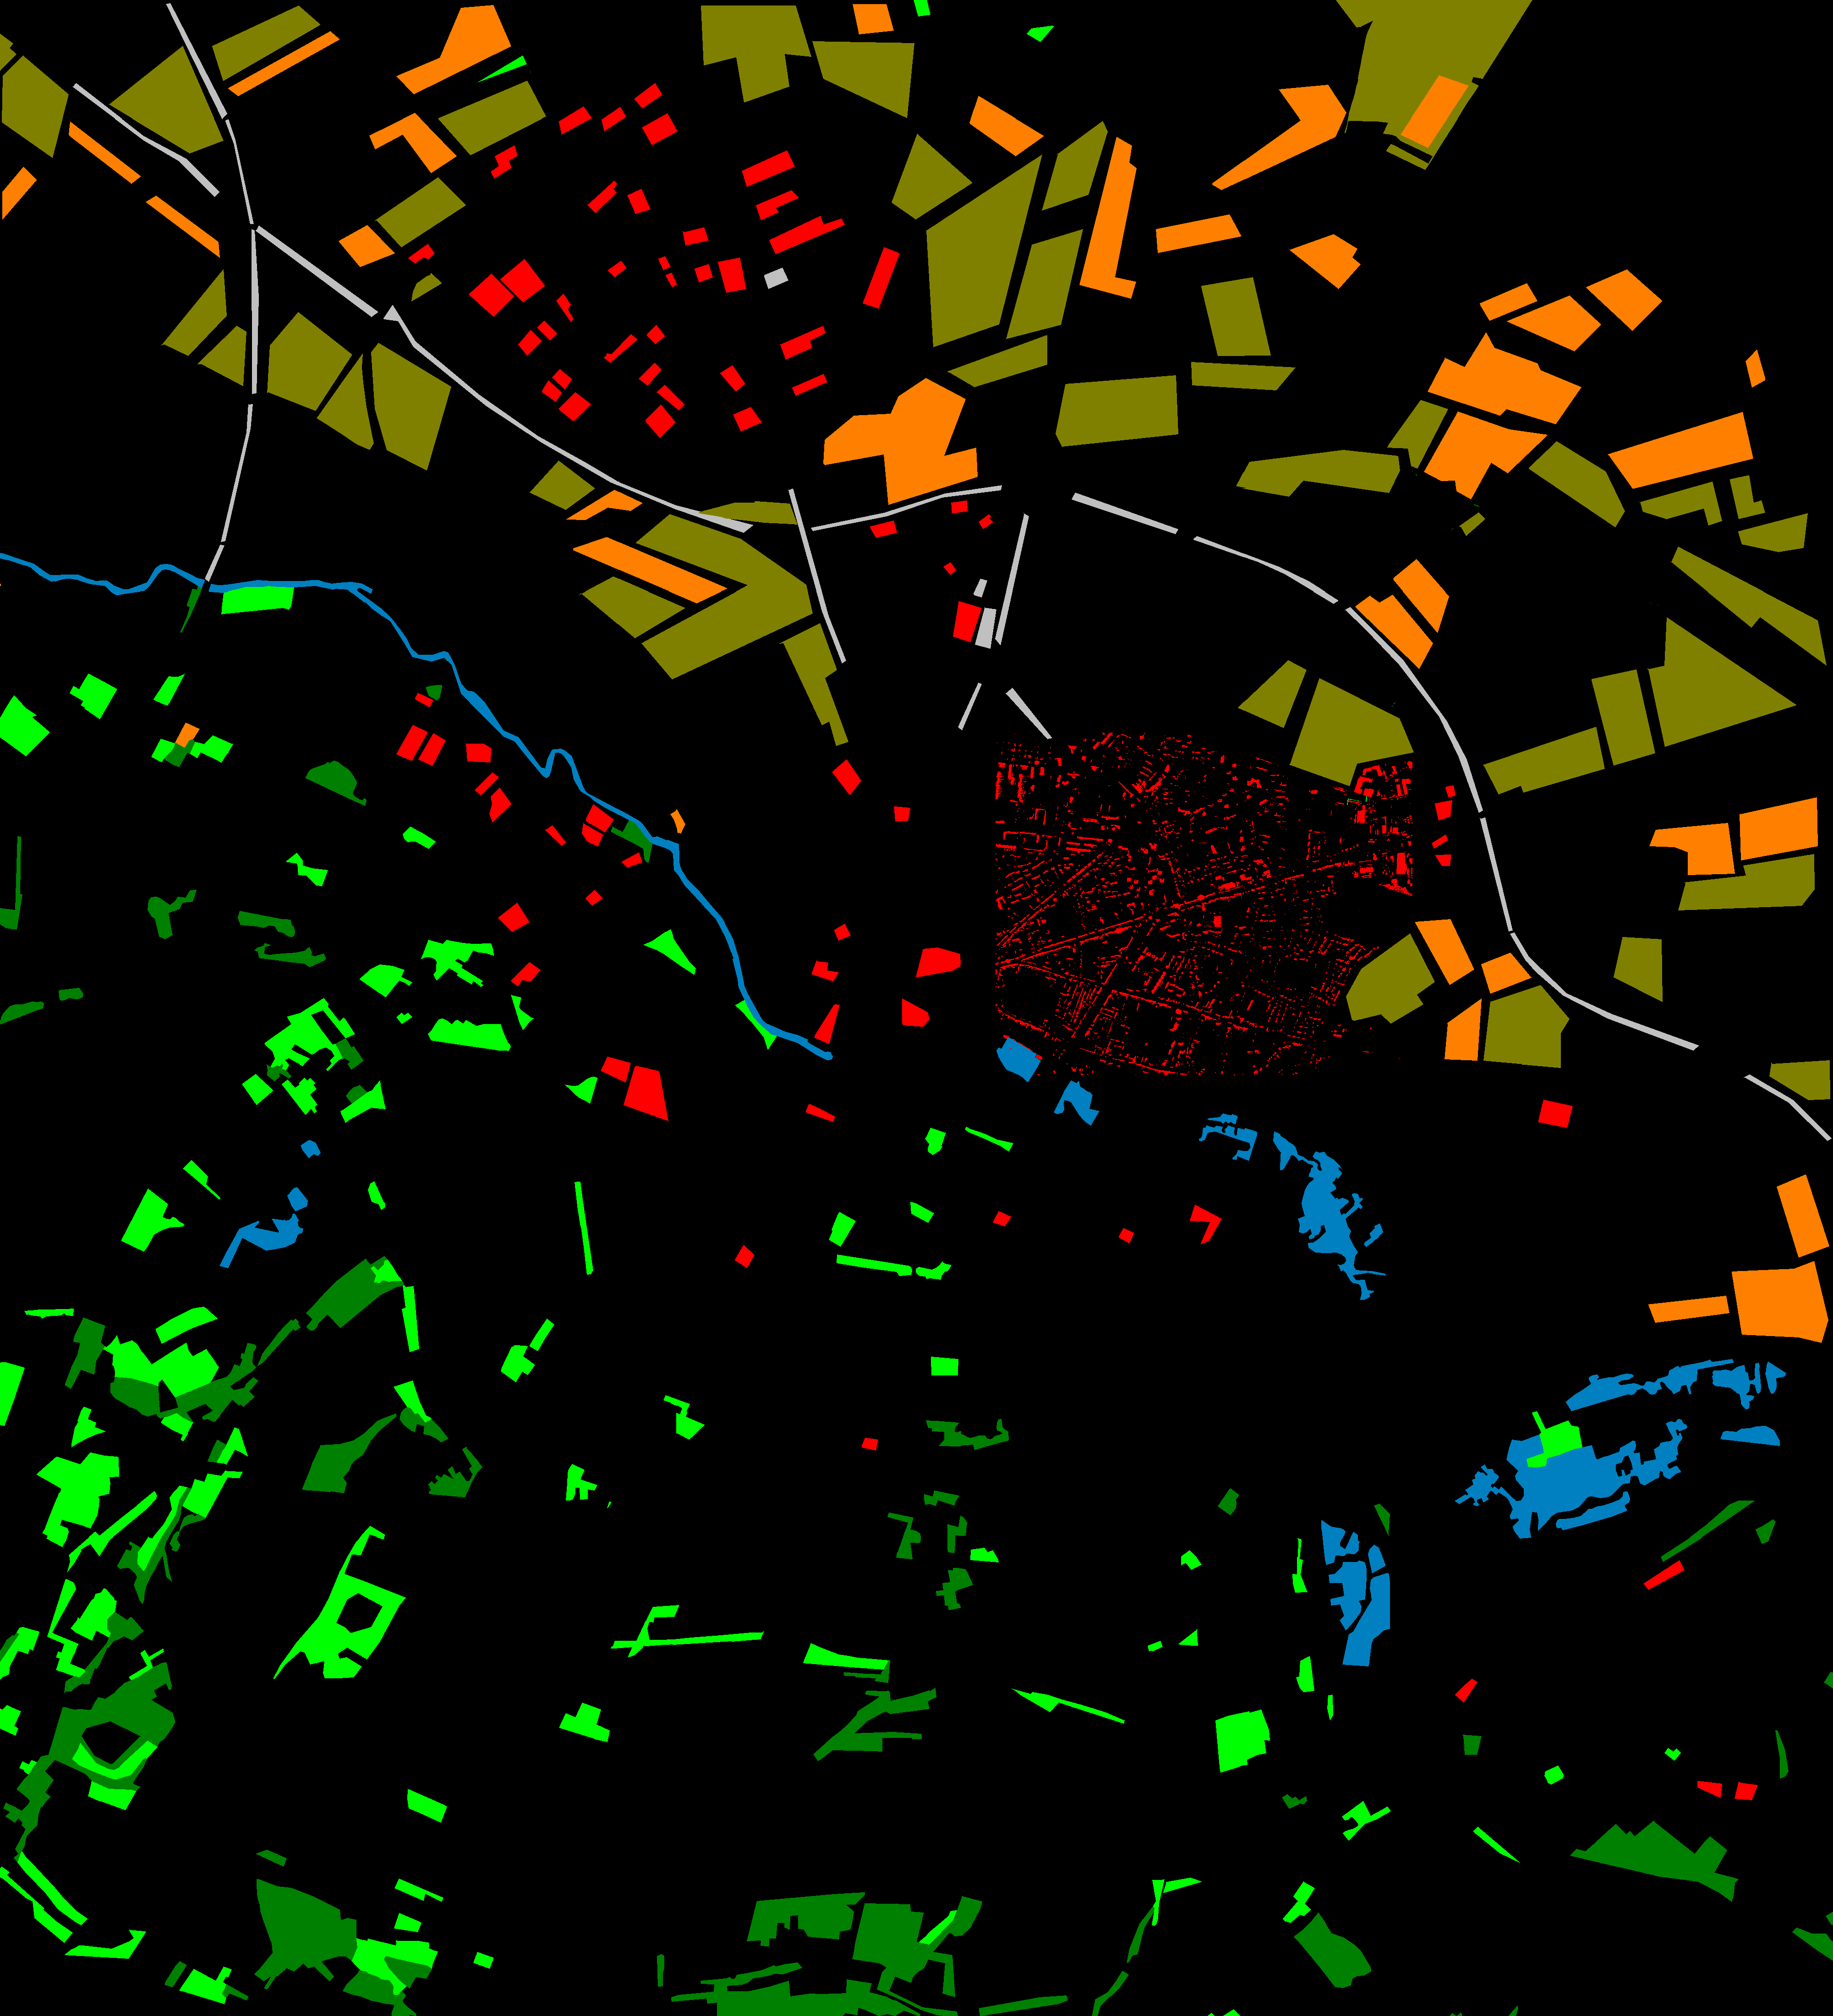
\includegraphics[width=0.4\textwidth]{GT_Amiens2012_2_5m_7classes_TR}}
     \hspace{4mm}
    \subfigure[Legenda classi della mappa di \emph{training}]{
      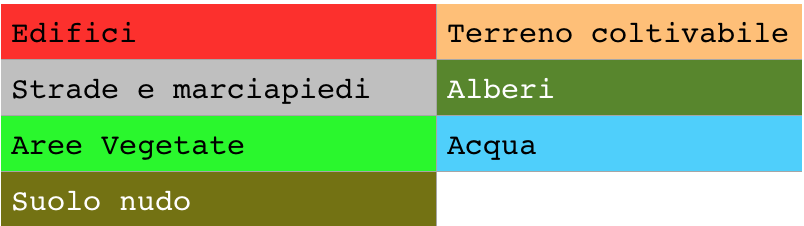
\includegraphics[scale=0.5]{Leggenda_7classi}}
    \caption{\emph{Dataset} con immagine RBG in falso colore ($4000\times4400$ pixel) acquisita su Amiens (Francia) dal sensore \textsc{SPOT5 HRG} nel 2012}
    \label{fig: Amiens122_5m}
  \end{figure}
\clearpage

\section{Descrizione del classificatore SVM}
Il classificatore usato è un classificatore \emph{soft-margin} SVM con $C=X$ e \emph{kernel} gaussiano a $\sigma = $. L'implementazione usata è una variante \emph{ad hoc} della \texttt{LIBSVM} [RIF] scritta in \texttt{C++}.\\
Il setup utilizzato per la fase di classificazione è composto da un \texttt{MacBookPro Retina} con un processore dual core Intel Core i5 $2.8$ GHz e $16$ GB di memoria e un iMac con processore quad core Intel Core i7 $3.4$ GHz e $8$ GB di memoria. \\

La fase di \emph{training} della SVM, la quale ha complessità temporale $O(n^\alpha)$ polinomialmente proporzionale al numero di vettori di \emph{training}, ha impiegato, in media, 30 minuti per completare l'ottimizzazione dei parametri, mentre la fase di etichettatura (con complessità $O(n)$ dove $n$ è il numero di vettori da etichettare) ha impiegato, in media, un'ora.

%

\section{Descrizione parametri per estrazione di \emph{feature} di tessitura}
Qui di seguito verranno presentate le variazioni di precisione del nostro algoritmo al variare delle diverse combinazioni dei parametri in gioco, evidenziando le motivazioni alla base delle nostre scelte progettuali.

\subsection{Pulitura del rumore(da rifinire)}
La pulitura del rumore è stata effettuata, come già illustrato in figura[], tramite un filtraggio passa-basso attraverso una gaussiana bi-dimensionale avente varianza $\sigma$ pari a 2 pixel e media nulla. Si può chiaramente vedere dalla tabella, come, applicando questa gaussiana sia sull'immagine in ingresso all'algoritmo HOG sia sulle immagini HOG risultanti, si abbia un incremento della \emph{overall accuracy} pari a ....

\subsection{Calcolo dei gradienti}
Per quanto riguarda la scelta della maschera da utilizzare per il calcolo del gradiente, sono state valutate diverse opzioni, tra cui la semplice maschera in $1D$ a differenze separate $[-1, 0 ,1]^T$, la maschera cubica $[1,-8,0,8,-1]$ e filtri  $2D$ più classici come le matrici di Prewitt e Sobel.\\
I risultati migliori sono stati ottenuti con il \emph{kernel} più semplice a $1D$ $3\times1$. Variazioni sulla maschera utilizzata non hanno modificato così tanto i risultati per giustificare un aumento computazionale dovuto all'utilizzo di filtri più complessi. Per questo motivo abbiamo deciso di utilizzare in tutti e tre i casi la soluzione più semplice e ottimale.\\

La fase del gradiente è stata considerata tra $0$ e $180$ (ignorandone quindi il segno) in quanto le strutture geometriche di cui ci interessa avere informazioni (quali strade, fiumi, \ldots) possono essere identificate univocamente dalla direzione e non è invece rilevante il verso del gradiente.

\subsection{Numero di canali dei vettori delle \emph{feature}}
Per quanto riguarda il numero di canali utilizzati per l'istogramma, la scelta che ha fornito prestazioni migliori è risultata essere quella con numero di bande pari a 4. Un aumento del numero di \emph{bins} comporta un aumento della risoluzione angolare e, pur apportando complessivamente poca informazione aggiuntiva,  aumenta la dimesionalità dello spazio delle \emph{feature} $\mathbb{R}^d$. Infatti, in primo luogo, all'aumentare di $d$, cresce la complessità computazionale del classificatore, che si traduce in un allungamento dei tempi di calcolo e in una maggiore occupazione di memoria.

\subsection{Dimensione delle celle}
La scelta di utilizzare celle di elevate dimensioni introduce un'alta correlazione tra i vettori delle \emph{feature}, mentre un' eccessiva riduzione comporta l'inserimento di vettori così scorrelati da avere valori praticamente associabili a rumore. La giusta via di mezzo è stata trovata empiricamente attraverso diverse sperimentazioni ed è risultata essere diversa (come ci si può aspettare) a seconda della risoluzione spaziale con cui si operava:
\begin{itemize}
\item cella da $4\times 4$ pixel per immagini a risoluzione $2000 \times 2200$ (\ref{fig: Amiens65m})
\item cella da $2 \times 2$ pixel per immagini a risoluzione $4001 \times 4400$ (\ref{fig: Amiens62_5m} e\ref{fig: Amiens122_5m} )
\end{itemize}

\subsection{Dimensione dei blocchi}
Si è deciso di mantenere costante il numero di pixel usati per la normalizzazione dei blocchi ad un valore di $16\times16$, dal momento che questo valore non inficia la quantità di informazione a disposizione.

\clearpage
\section{Discussione dei risultati}
\subsection{Amiens 2006 - 5m - 10 classi}
\'E riportata in Figura \ref{fig:ClassMap_Amiens2006_5m} la mappa di classificazione con \emph{feature} HOG aggiuntive in configurazione di $4$ \emph{bins}, celle di dimensione $4\times4$ pixel e blocchi di normalizzazione con $16\times16$ pixel, con filtraggio gaussiano sia per l'immagine in ingresso che per le immagini HOG.
\begin{figure}[!ht]
 \center
 \subfigure{
      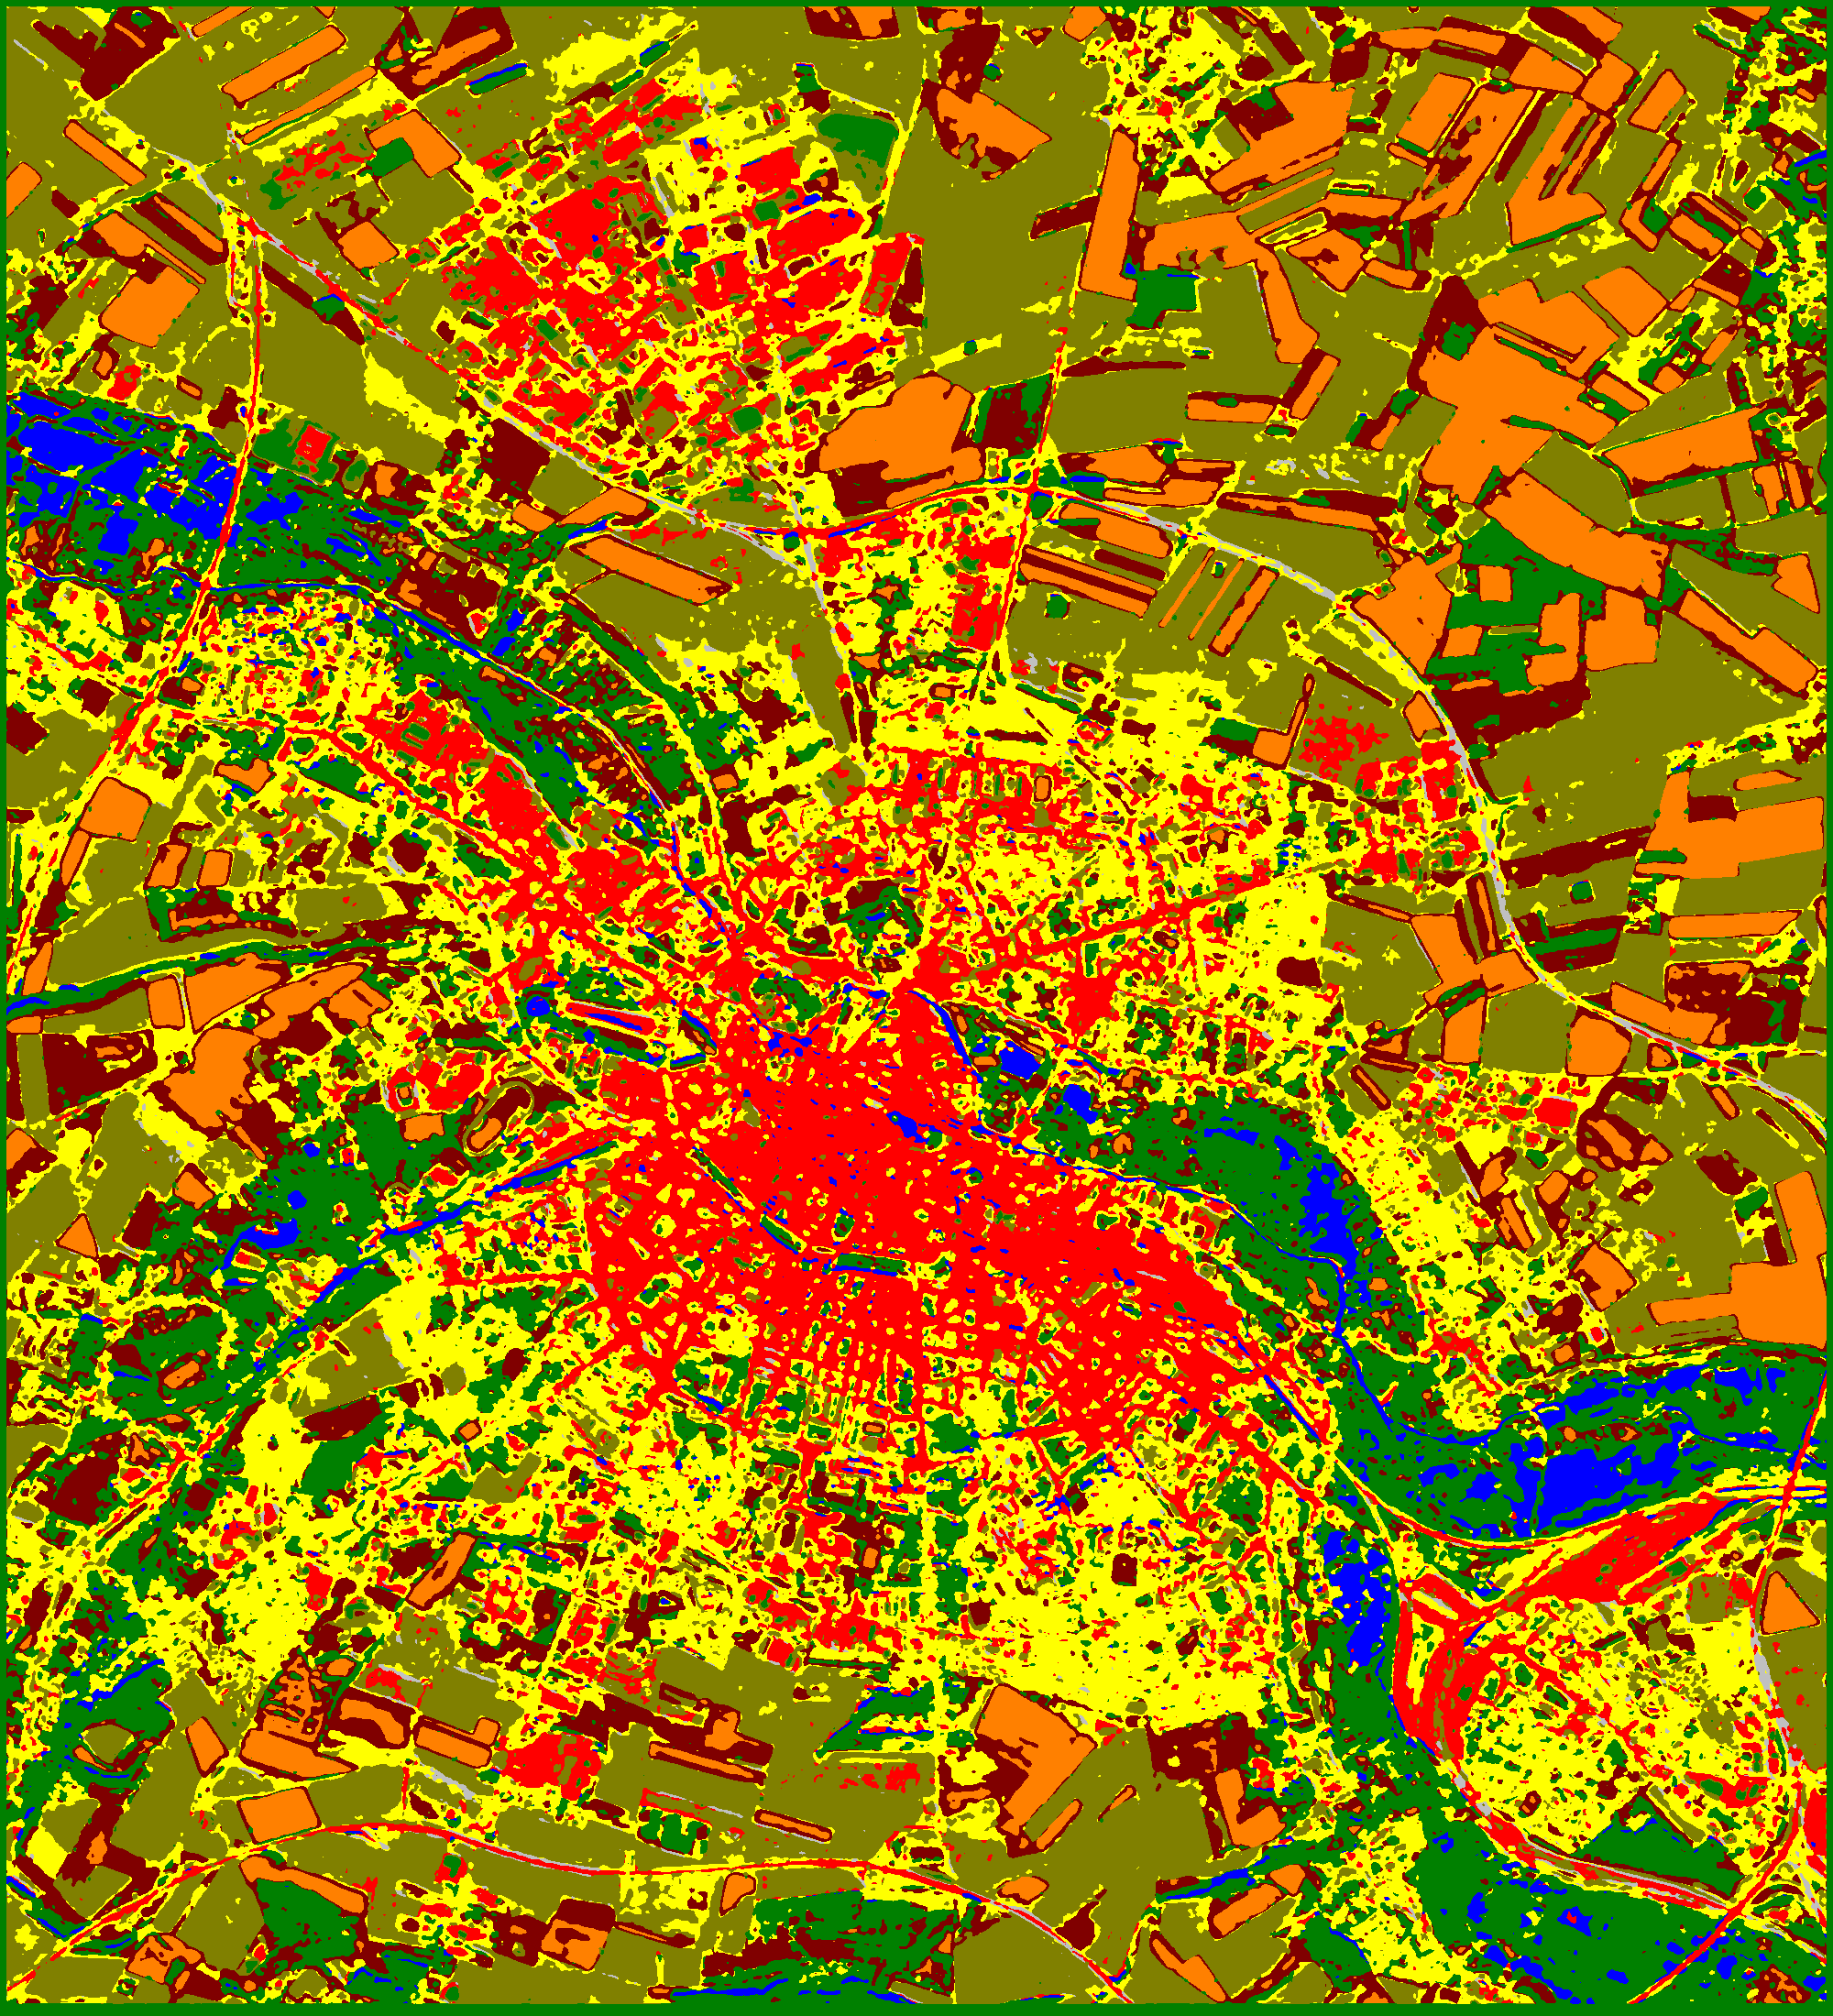
\includegraphics[width=0.7\textwidth]{ClassMap_Amiens2006_5m}}
      \\
      \subfigure{
      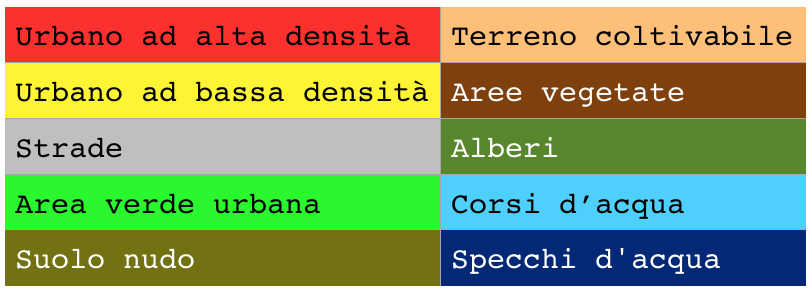
\includegraphics[width=0.35\textwidth]{Leggenda_2006_10classi}}
     
    \caption{Mappa di classificazione del \emph{dataset} \emph{Amiens 2006 - 5m - 10 classi}}
    \label{fig:ClassMap_Amiens2006_5m}
  \end{figure} 
 
Da una prima sommaria analisi visiva, si può chiaramente constatare come nel complesso la mappa di classificazione sia soddisfacente, sebbene si noti già adesso difficoltà nella classificazione delle strade (classe 3) soprattutto all'interno dell'area urbana. Inoltre, è evidente che la classe relativa ai corsi d'acqua (classe 9) non è presente (o almeno non apprezzabile).\\

Queste prime impressioni vengono confermate anche dall'analisi numerica della matrice di confusione (Figura \ref{fig:Matrice_di_confusione_Amiens2006_5m_HOG}). 
\begin{figure}[!ht]
    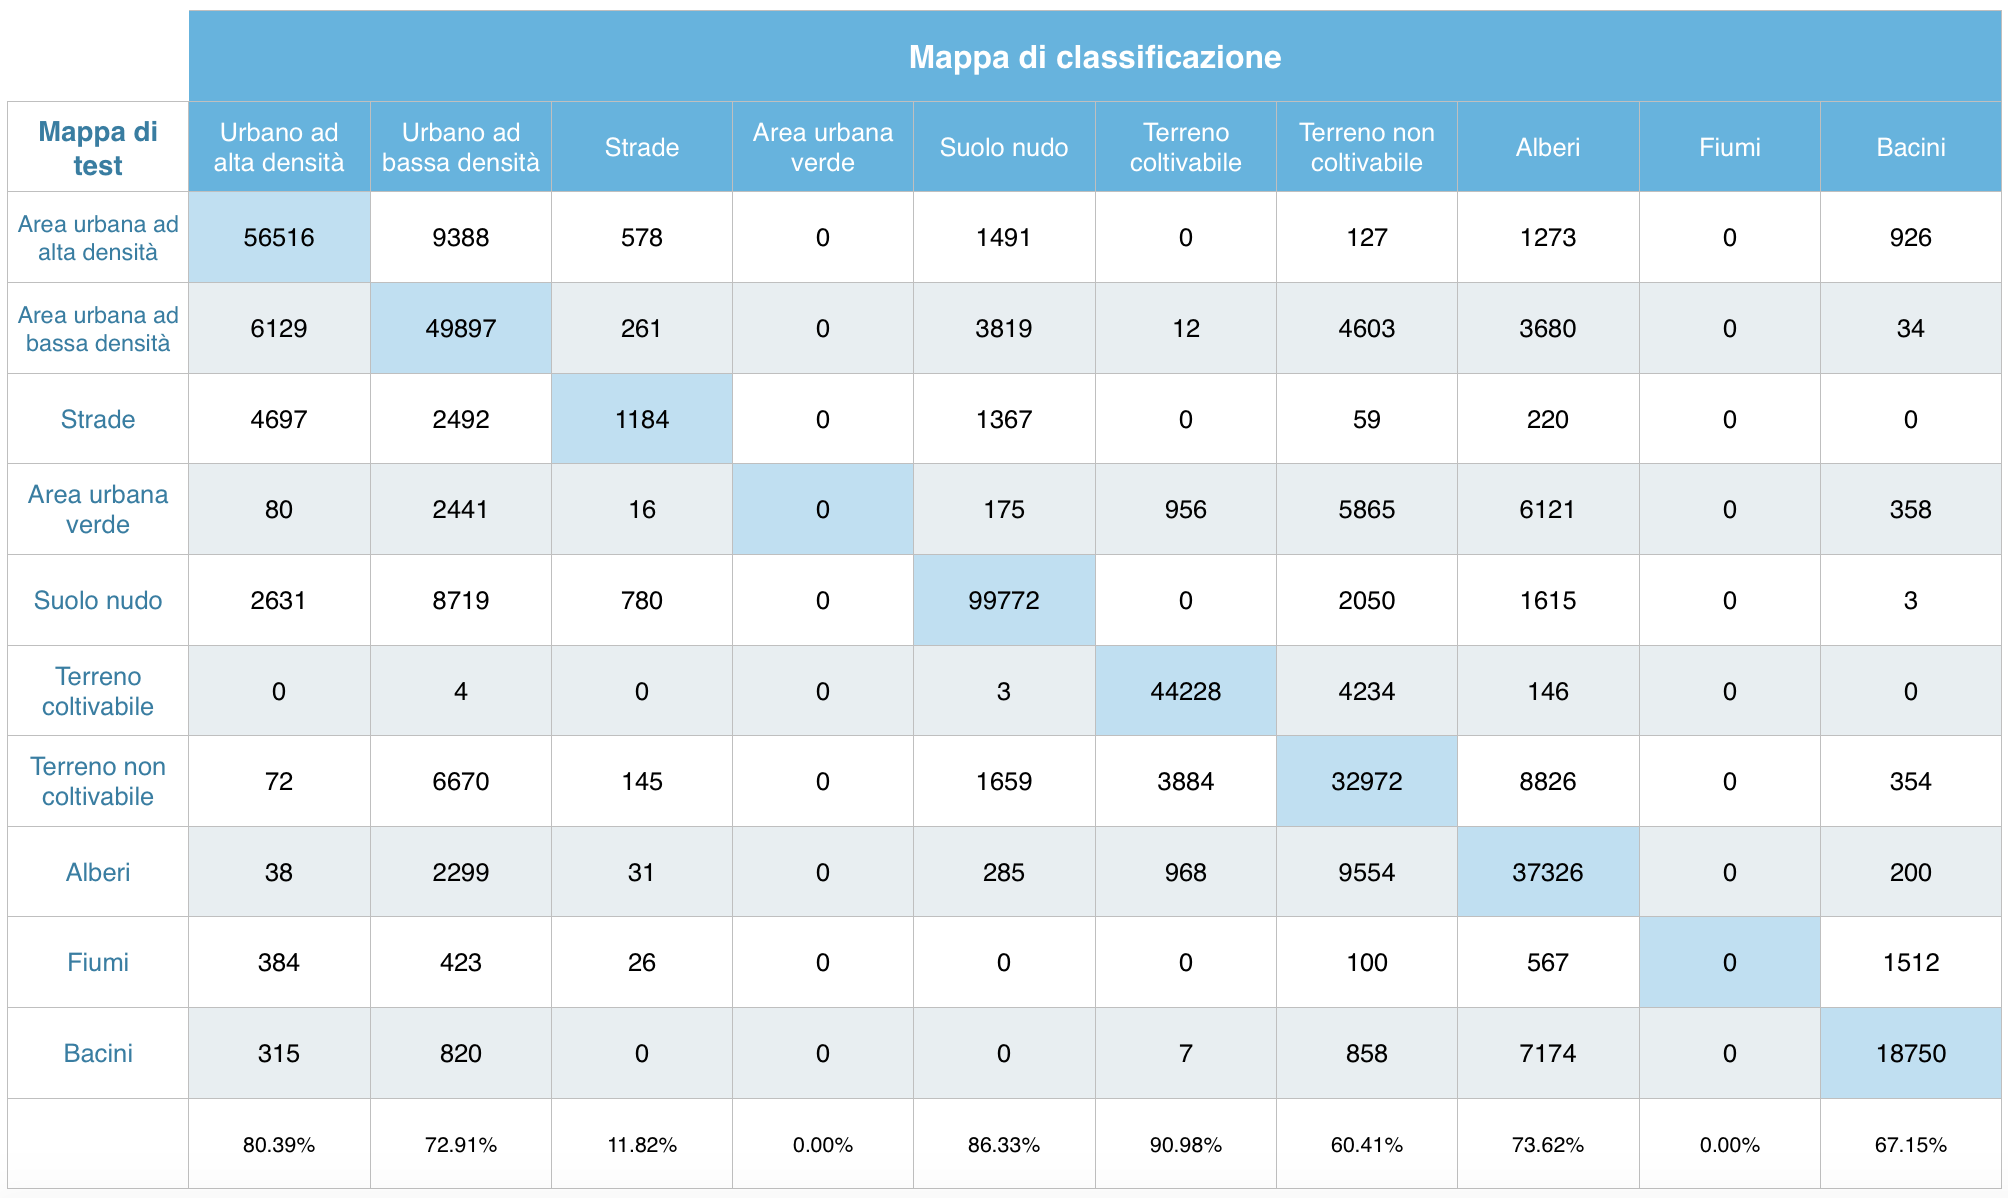
\includegraphics[width=1\textwidth]{Matrice_di_confusione_Amiens2006_5m_HOG}
    \caption{Matrice di confusione della sessione di classificazione del dataset \emph{Amiens 2006 - 5m - 10 classi}}
    \label{fig:Matrice_di_confusione_Amiens2006_5m_HOG}
\end{figure}

Analizzando la matrice di confusione saltano subito all'occhio alcuni comportamenti interessanti nella classificazione. La zona urbana (classe 1 e 2) viene discriminata in modo soddisfacente (con accuratezze nell'ordine del $75\%$); ciò che si perde nell'accuratezza deriva in massima parte dalla difficoltà del classificatore di distinguere le aree urbane di diversa densità.\\
L'analisi quantitativa della matrice di confusione conferma quanto già ipotizzato precedentemente,  ovvero che le strade sono quasi del tutto perse registrando un'accuratezza di circa $11\%$, a scapito sopratutto dell'area urbana. \\
Si è registrata un'ottima \emph{performace} nelle classificazioni di aree più uniformi quali suolo nudo (classe 5) e terreni coltivabili e non (classi 6 e 7): pochissimi sono i pixel etichettati in modo errato per queste regioni.\\
Tuttavia, il classificatore ha avuto serie difficoltà in quelle zone minoritarie dove il numero di pixel di training erano inferiori. In particolare, vengono completamente perse l'area verde urbana e i corsi d'acqua ($0\%$), le cui etichette sono state assegnate in maggioranza alla classe alberi e alla classe  bacini d'acqua, rispettivamente.\\
La difficoltà di classificazione di questo \emph{dataset} risiede soprattutto nella sovrabbondanza del numero di classi da distinguere, in quanto molti errori fatti nella mappa di classificazione sono proprio causati dalla confusione di coperture di suolo simili tra loro.\\

In termini generali, l'\emph{Overall Accuracy} (OA) complessivo di questo primo \emph{dataset} è stato di $73.23\%$, mentre l'AA è risultato essere $54.36\%$. 
\\
Per concludere questa prima sessione di discussione, è interessante confrontare questi risultati con quelli ottenuti senza estrazione delle \emph{feature} HOG. La Figura \ref{fig:Confronto_Amiens2006_5m} sintetizza i miglioramenti/peggioramenti classe per classe.
 
 \begin{figure}[!ht]
      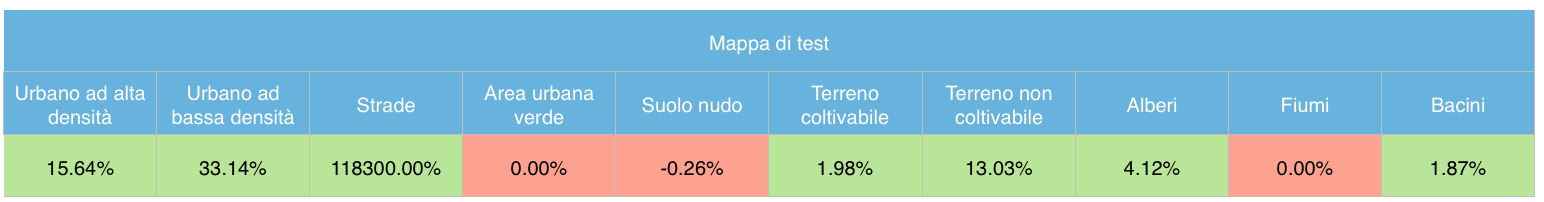
\includegraphics[width=1\textwidth]{Confronto_Amiens2006_5m}
    \caption{Confronto percentuale tra accuratezze classe per classe con e senza estrazione di \emph{feature}}
    \label{fig:Confronto_Amiens2006_5m}
  \end{figure}
Si può chiaramente osservare che l'introduzione delle \emph{feature} HOG ha quasi sempre apportato miglioramenti, con benefici notevoli soprattutto per le classi di suolo urbano. La Figura \ref{fig:Confronto_Amiens2006_5m} dimostra come effettivamente il risultato della classificazione dell'immagine a tre canali mostri in generale più dettaglio; così facendo, però, ciò che si guadagna in risoluzione si perde in accuratezza nella classificazione, in quanto molti pixel urbani vengono etichettati come appartenenti ad altre classi (in particolare la classe 10, rappresentata dal bianco nelle immagini).

 \begin{figure}[!ht]
 \center
   \subfigure[Mappa di classificazione con HOG]{
      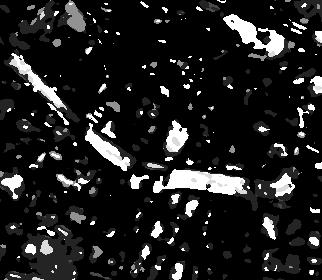
\includegraphics[width=0.4\textwidth]{ClassMap_Amiens2006_5m_HOG}}
\hspace{2mm}      
      \subfigure[Mappa di classificazione senza HOG]{
      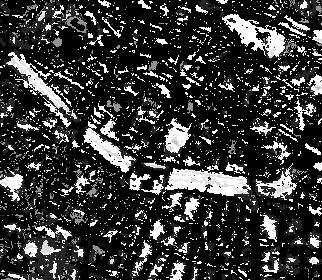
\includegraphics[width=0.4\textwidth]{ClassMap_Amiens2006_5m_riferimento}}
    \caption{Confronto su una porzione dell'area urbana di $250\times250$ pixel della mappa di classificazione con e senza estrazione di \emph{feature} HOG sul \emph{dataset} Amiens 2006 a $5$ m}
    \label{fig:confrontoAmiens2006_5m}
  \end{figure}


\clearpage

%\subsection{Amiens 2006 - 2.5m - 7 classi}
%Come già introdotto nel caso precedente, anche per questo esperimento
%foto-interpretativa 
%\clearpage

\subsection{Amiens 2012 - 2.5m - 7 classi}
\'E riportata in Figura \ref{fig:ClassMap_Amiens2012_2_5m_noroads} la mappa di classificazione con \emph{feature} HOG aggiuntive in configurazione di $4$ \emph{bins}, celle di dimensione $2\times2$ pixel e blocchi di normalizzazione con $16\times16$ pixel, con filtraggio gaussiano sia per l'immagine in ingresso che per le immagini HOG.
\begin{figure}[!ht]
 \center
 \subfigure{
      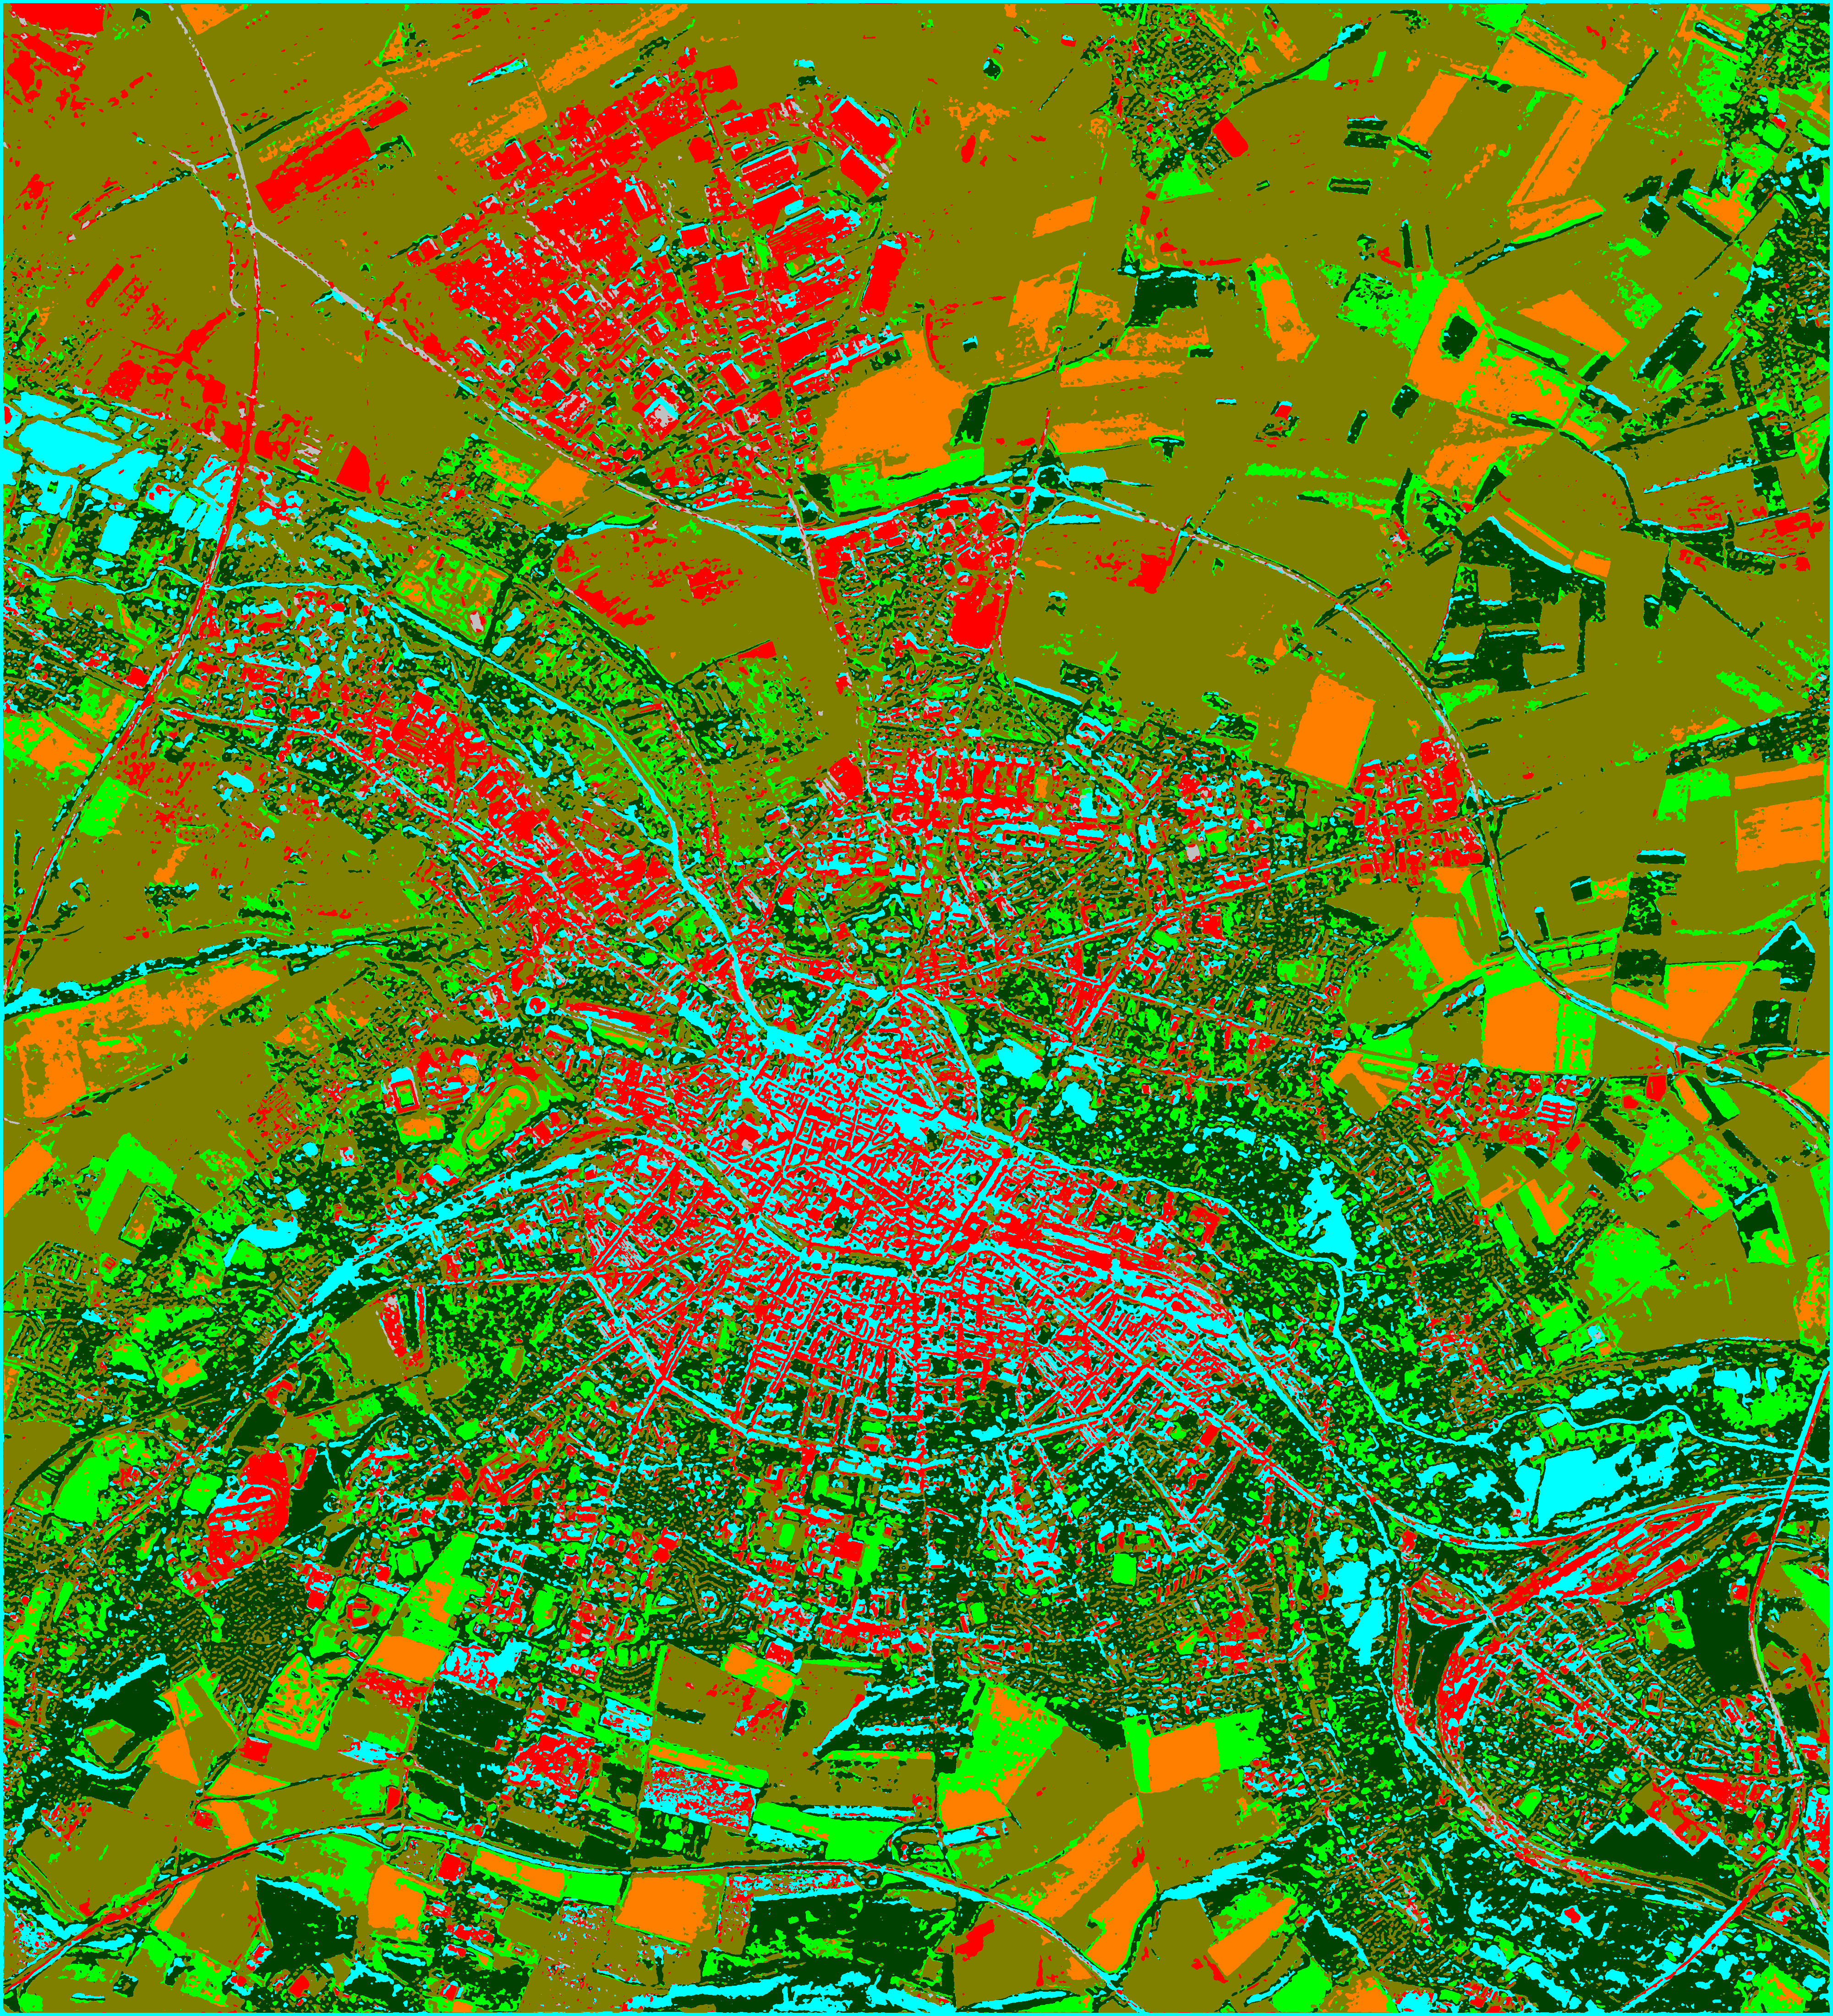
\includegraphics[width=0.7\textwidth]{ClassMap_Amiens2012_2_5m_noroads}}
      \\
      \subfigure{
      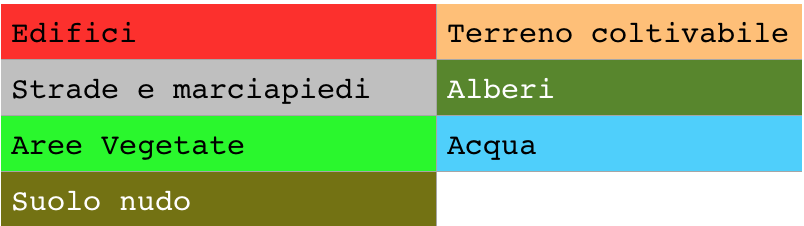
\includegraphics[width=0.35\textwidth]{Leggenda_7classi}}
     
    \caption{Mappa di classificazione del dataset \emph{Amiens 2012 - 2.5m - 7 classi}}
    \label{fig:ClassMap_Amiens2012_2_5m_noroads}
  \end{figure} 

\'E importante far notare fin da subito che l'immagine telerilevata che fa parte di questo \emph{dataset} è stata acquisita in situazioni ambientali e in periodi di tempo diversi da quelle precedenti (nell'inverno 2012). Questo costituisce un evidente deficit nell'informazione proveniente dal suolo, in quanto la presenza di neve uniformemente distribuita nell'area di interesse ha reso altamente più complesso la discriminazione delle 7 diverse coperture di suolo.\\

Già con un'analisi della mappa, si osserva che qualitativamente il risultato sembra peggiorare rispetto ai due esperimenti precedenti. Due sono i punti critici già a prima vista apprezzabili:
\begin{itemize}
\item i pixel etichettati come appartenenti al suolo nudo (classe 4) sono in misura sovrabbondante rispetto ai risultati precedenti: ciò può essere giustificato dall'uniformità del suolo introdotta dal manto nevoso;
\item la quasi totale scomparsa delle strade (classe 2) nel centro, che quasi ovunque vengono classificate come pixel appartenenti alla classe acqua (classe 7) GIUSTIFICAZIONE
\end{itemize}

Queste considerazioni trovano conferma  negli indici di accuratezza  che raggiungono valori meno soddisfacenti rispetto ai casi esaminati in precedenza.
L'OA per questo esperimento, infatti, si è fermata al $56.63\%$, mentre l'AA ha raggiunto il valore di  solo $57.33\%$.\\
 In Figura \ref{fig:Matrice_di_confusione_Amiens2012_5m_HOG_without_roads} viene presentata la matrice di confusione di questo esperimento.
\\
\begin{figure}[!ht]
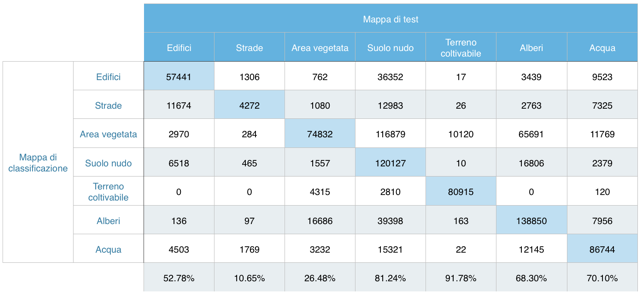
\includegraphics[width=1\textwidth]{Matrice_di_confusione_Amiens2012_5m_HOG_without_roads}
\caption{Matrice di confusione della sessione di classificazione del \emph{dataset} \emph{Amiens 2012 - 5m - 7 classi}}
\label{fig:Matrice_di_confusione_Amiens2012_5m_HOG_without_roads}
\end{figure}
\
\\
Si può osservare che la classe per la quale la classificazione ha ottenuto i risultati migliori è stata quella relativa al terreno coltivabile (classe 5), che ha registrato un accuratezza del $90\%$. Prestazioni soddisfacenti sono state raggiunte anche per le classi di suolo nudo e acqua (classi 4 e 7), in cui una buona percentuale di pixel della mappa di classificazione coincide con la verità al suolo.\\

% \begin{figure}[!ht]
%\center 
%   \subfigure[Mappa di classificazione senza HOG]{
%   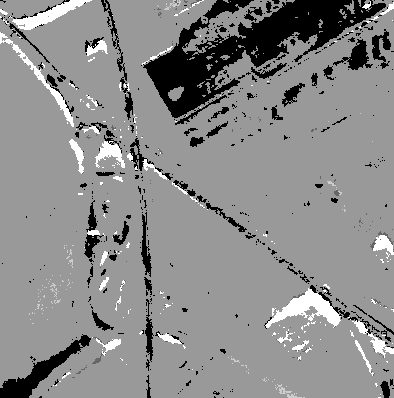
\includegraphics[width=0.4\textwidth]{ClassMap_Amiens2012_2_5m_riferimento}
%   }
%   \hspace{3mm}
%   \subfigure[Mappa di classificazione con HOG]{
%   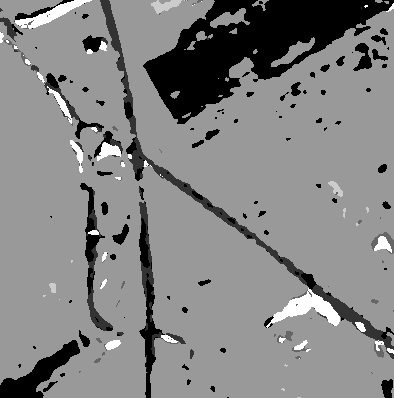
\includegraphics[width=0.4\textwidth]{ClassMap_Amiens2012_2_5m_HOG}
%   }
%      
%    \caption{Confronto su una porzione dell'area urbana di $250\times250$ pixel della mappa di classificazione con e senza estrazione di \emph{feature} HOG sul \emph{dataset} Amiens 2012 a $2.5$ m }
%    \label{fig:confrontoAmiens2012_2_5m}
%  \end{figure}

\begin{figure}[!ht]
      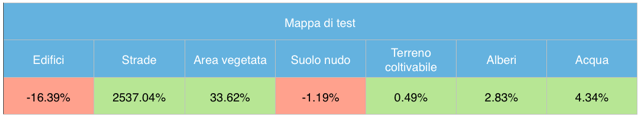
\includegraphics[width=1\textwidth]{Confronto_Amiens2012_con_e_senza_hog}
    \caption{Confronto percentuale tra accuratezze classe per classe con e senza estrazione di \emph{feature} per il \emph{dataset} Amiens 2012 a $2.5$ m}
    \label{fig:Confronto_Amiens2012_2.5m}
  \end{figure}

Confrontando i risultati ottenuti dalla classificazione con HOG e da quella avente come \emph{feature} le sole tre bande telerilevate, si osserva come, anche questa volta, l'introduzione degli HOG porti, in generale, ad un incremento della percentuale di pixel classificati correttamente: in particolare in Figura \ref{fig:Confronto_Amiens2012_2.5m} si può notare un netto miglioramento ($+2537\%$) per le strade, benché in termini assoluti restino ancora ben poco classificate ($10\%$). Si è rilevato, tuttavia, un leggero peggioramento ($-16\%$) nell' individuazione degli edifici. \\ In conclusione la presenza degli HOG migliora anche OA e AA, seppure in maniera limitata. \\

Vista la non ancora soddisfacente percentuale di pixel di strada classificati in maniera adeguata, si è deciso di inserire una \emph{feature} aggiuntiva della struttura cartografica delle strade di Amiens. L'immagine binaria in Figura \ref{fig:immagine_roads} è stata inserita nel vettore delle \emph{feature} in coda all'immagine precedente con vettori HOG.
Quest'immagine è il risultato della fusione di tre mappe tematiche (strade principali, strade secondarie e binari ferroviari), ottenuta dal servizio di mappatura stradale della Urban Atlas European. In particolare l'immagine è aggiornata all'anno $2006$ e possiede una risoluzione spaziale di 5 m/pixel.

\begin{figure}[!ht]
\center
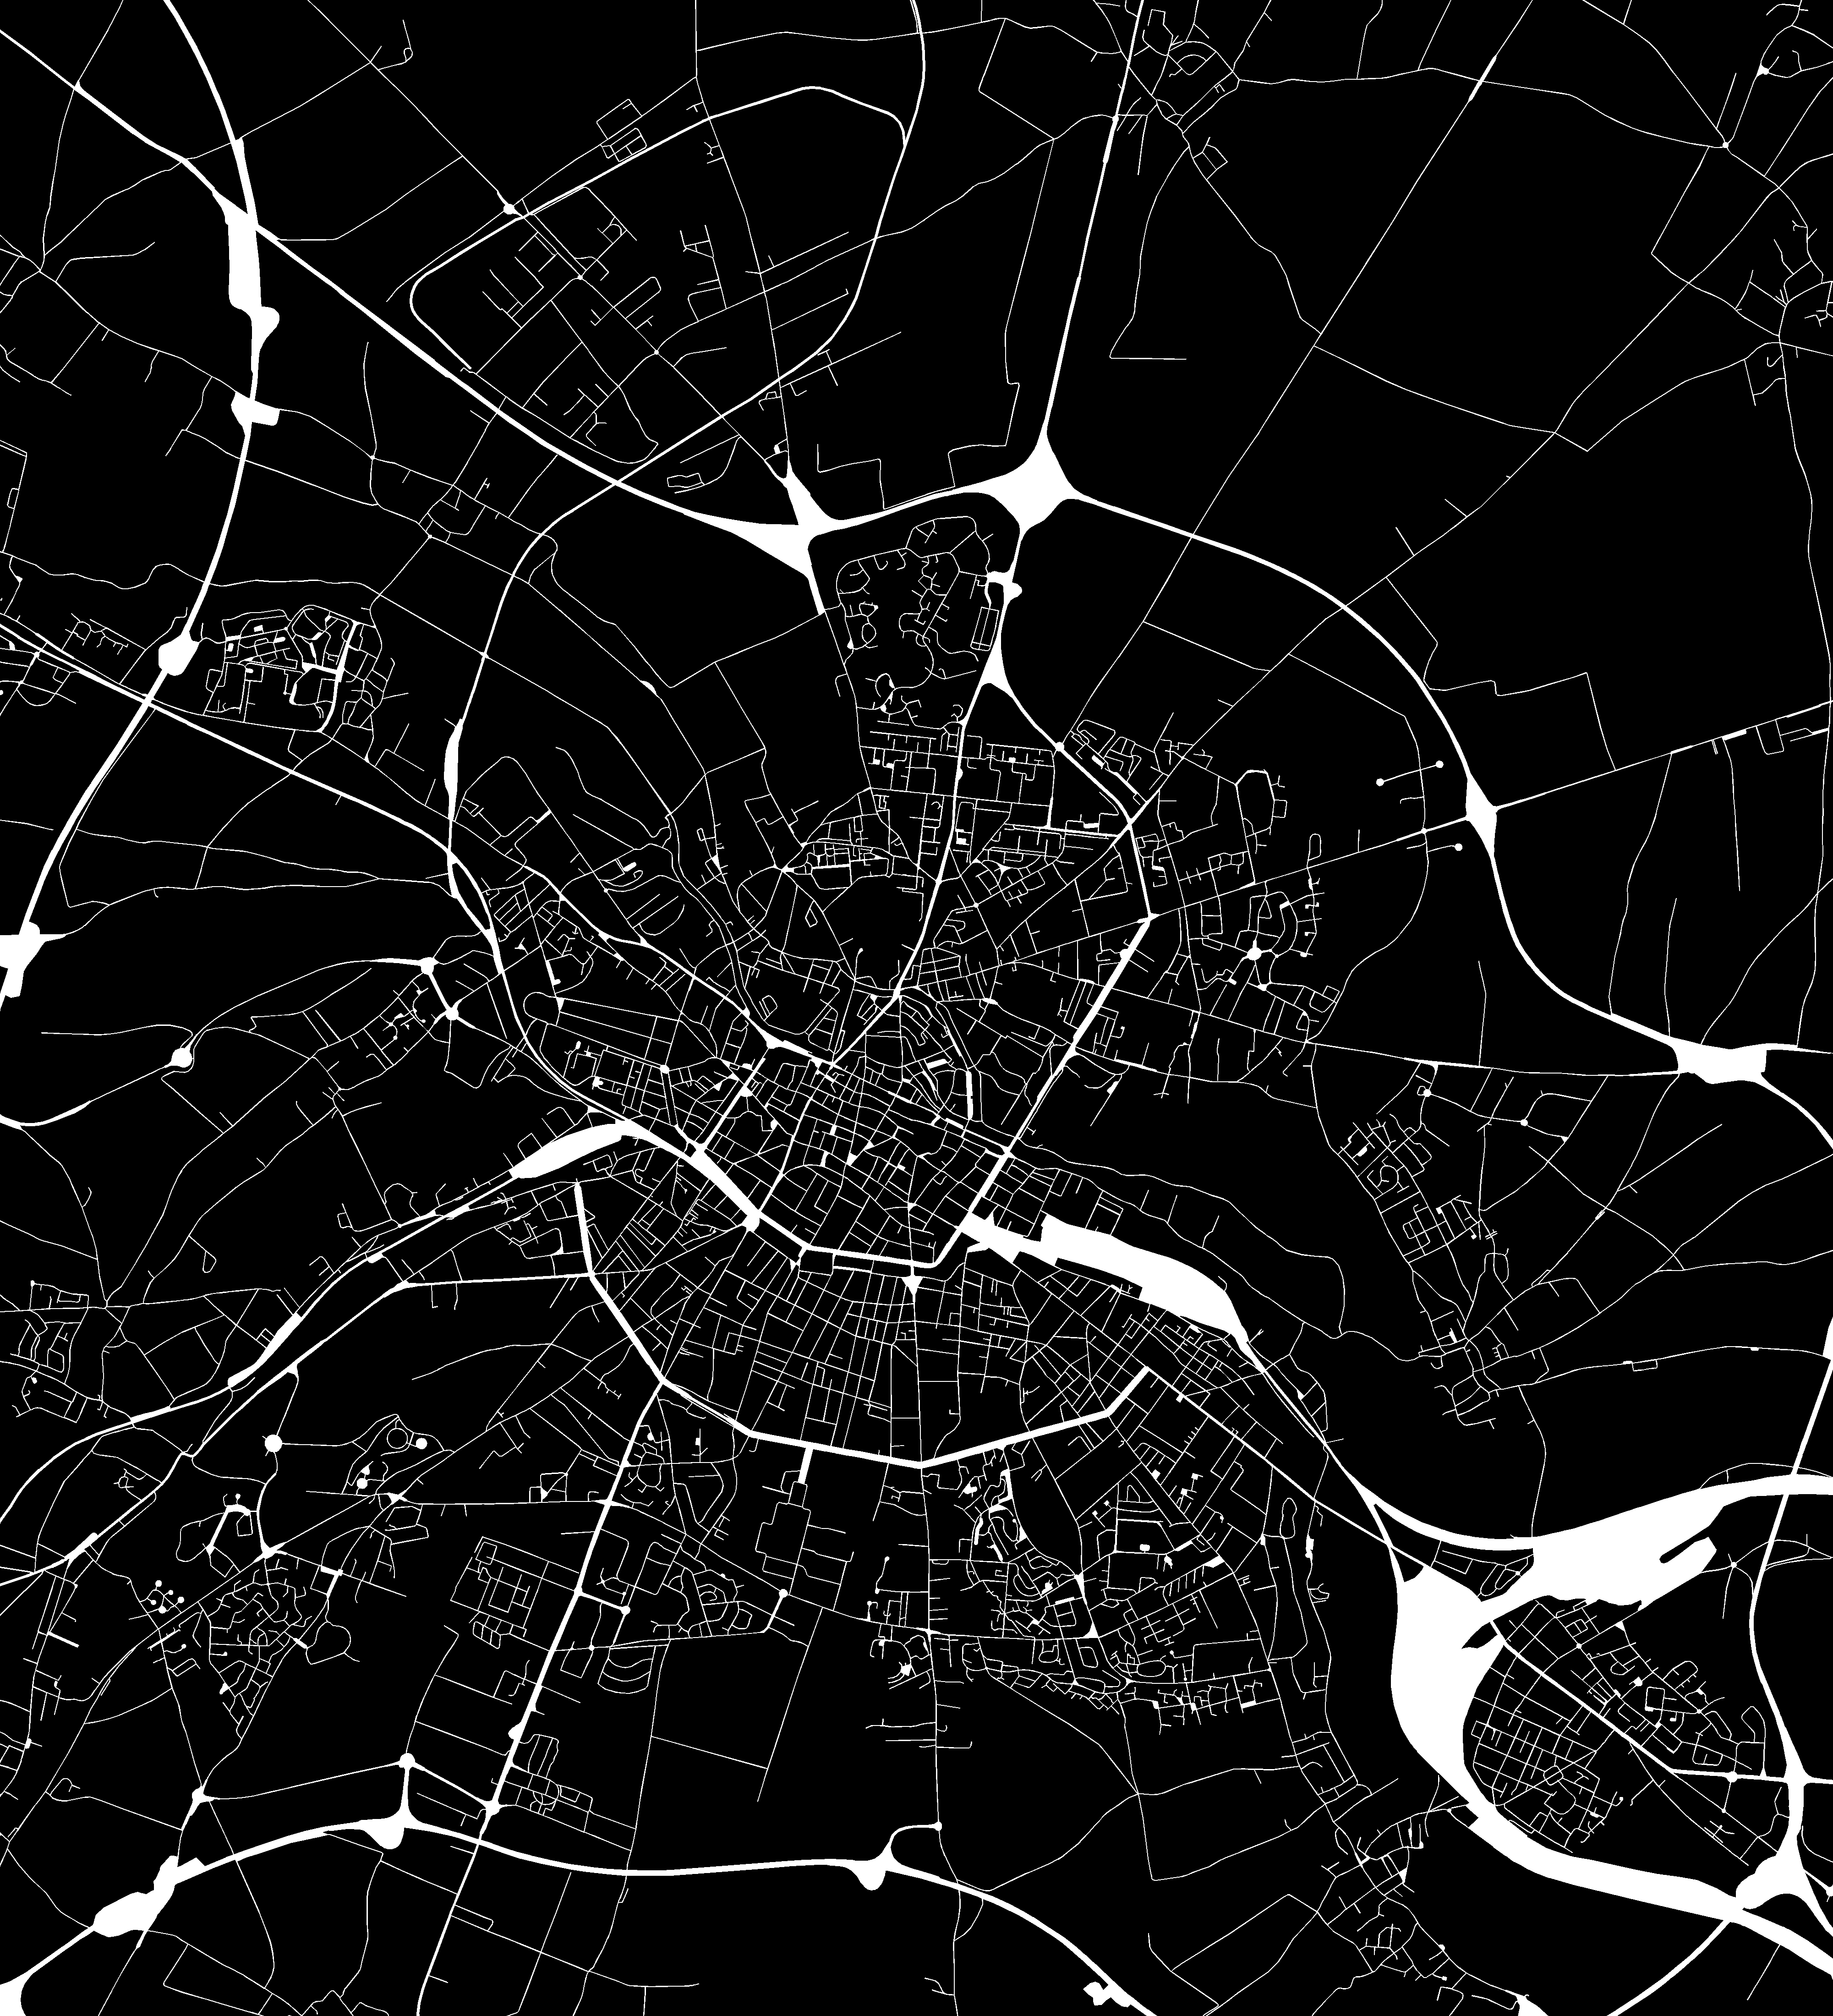
\includegraphics[width=0.5\textwidth]{amiens6_roads}
\caption{Immagine binaria della struttura cartografica delle strade di Amiens: le strade sono rappresentate con il  bianco e lo sfondo in nero.}
\label{fig:immagine_roads}
\end{figure}
\

 In questo modo, si è riusciti a limitare la degradazione della classe strade (classe 2) portandola ad un più che accettabile valore di accuratezza ($64.61\%$); dal momento che il numero di pixel classificati come strade non è molto significativo nella totalità dei pixel dell'immagine, non si ha un'apprezzabile incremento dell'OA, al contrario della AA che, pesando gli errori uniformemente, registra un significativo miglioramento ($63.54\%$).
In Figura ref[] viene mostrato l'effetto di questa \emph{feature} aggiuntiva per la classificazione delle strade.
% (la porzione di immagine utilizzata è la stessa della Figura \ref{fig:confrontoAmiens2012_2_5m}, per una più immediata comprensione).
 \begin{figure}[!ht]
\center 
   \subfigure[Mappa di classificazione senza HOG]{
   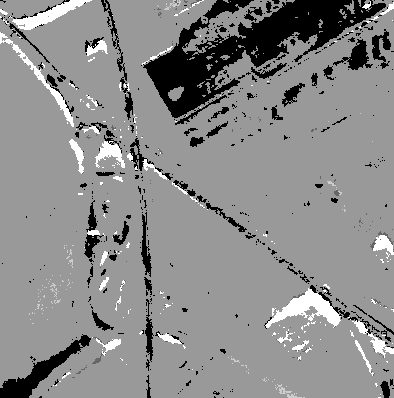
\includegraphics[width=0.4\textwidth]{ClassMap_Amiens2012_2_5m_riferimento}
   }
   \hspace{3mm}
   \subfigure[Mappa di classificazione con HOG]{
   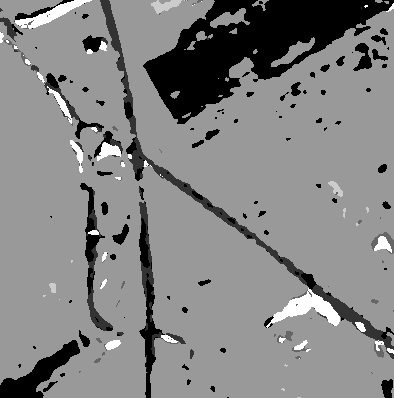
\includegraphics[width=0.4\textwidth]{ClassMap_Amiens2012_2_5m_HOG}
   }
      \\
     \subfigure[Mappa di classificazione con HOG e cartografia]{
   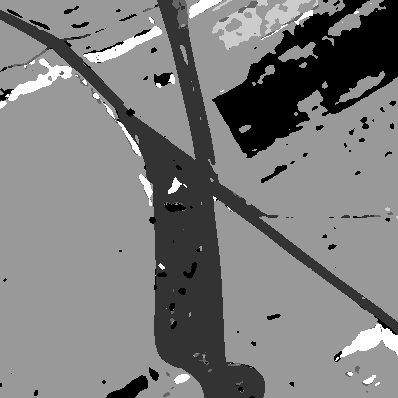
\includegraphics[width=0.4\textwidth]{ClassMap_Amiens2012_2_5m_HOG_and_roads}
   } 
    \caption{Confronto su una porzione della periferia di Amiens di $250\times250$ pixel della mappa di classificazione con e senza estrazione di \emph{feature} HOG e con l'aggiunta della cartografia stradale sul \emph{dataset} Amiens 2012 a $2.5$ m. }
    \label{fig:confrontoAmiens2012_2_5m}
  \end{figure}
  \clearpage
  

\subsection{Amiens 2006 - 2.5m - 7 classi}
\'E riportata in Figura \ref{fig:ClassMap_Amiens2006_2_5m_roadsandhog} la mappa di classificazione con \emph{feature} HOG aggiuntive in configurazione di $4$ \emph{bins}, celle di dimensione $2\times2$ pixel e blocchi di normalizzazione con $16\times16$ pixel, con filtraggio gaussiano sia per l'immagine in ingresso che per le immagini HOG e con l'aggiunta della \emph{feature} cartografica delle strade di Amiens.

\begin{figure}[!ht]
 \center
 \subfigure{
      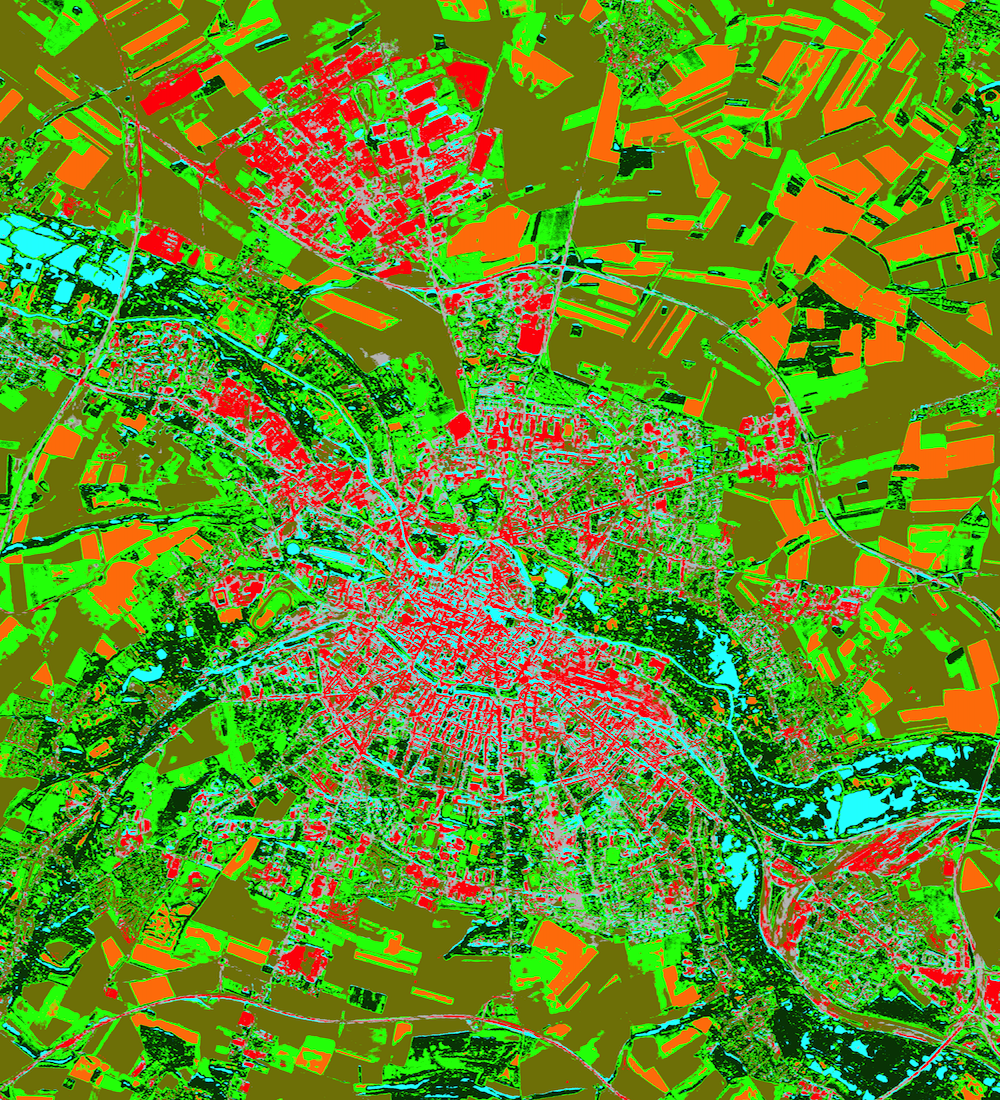
\includegraphics[width=0.7\textwidth]{ClassMap_Amiens2006_2_5m_roadsandhog}}
      \\
      \subfigure{
      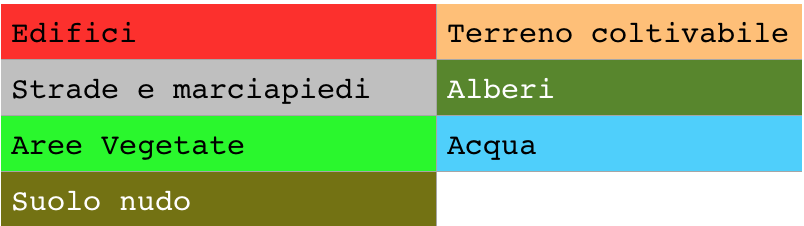
\includegraphics[width=0.35\textwidth]{Leggenda_7classi}}
     
    \caption{Mappa di classificazione del dataset \emph{Amiens 2006 - 2.5m - 7 classi}}
    \label{fig:ClassMap_Amiens2006_2_5m_roadsandhog}
  \end{figure} 

Su questo \emph{dataset} i risultati sono stati interessanti, poichè si differenziano notevolmente dai due casi studiati in precedenza.\\
E' innanzitutto importante far notare che questo esperimento ha registrato il valore più alto a livello di OA ($74.88\%$) e AA ($70.61\%$). \\
L'analisi della matrice di confusione (riportata in Figura \ref{fig:ClassMap_Amiens2006_2_5m_roadsandhog}) conferma il fatto che il classificatore, per questo \emph{dataset}, si comporti mediamente bene in tutte le classi, non mostrando grandi problemi a etichettare le 7 classi presenti.\\L'unico caso in cui i risultati non sono del tutto accettabili riguarda la distinzione tra area vegetata (classe 3) e alberi (classe 6), i cui pixel vengono spesso confusi tra le due categorie.

\begin{figure}[!ht]
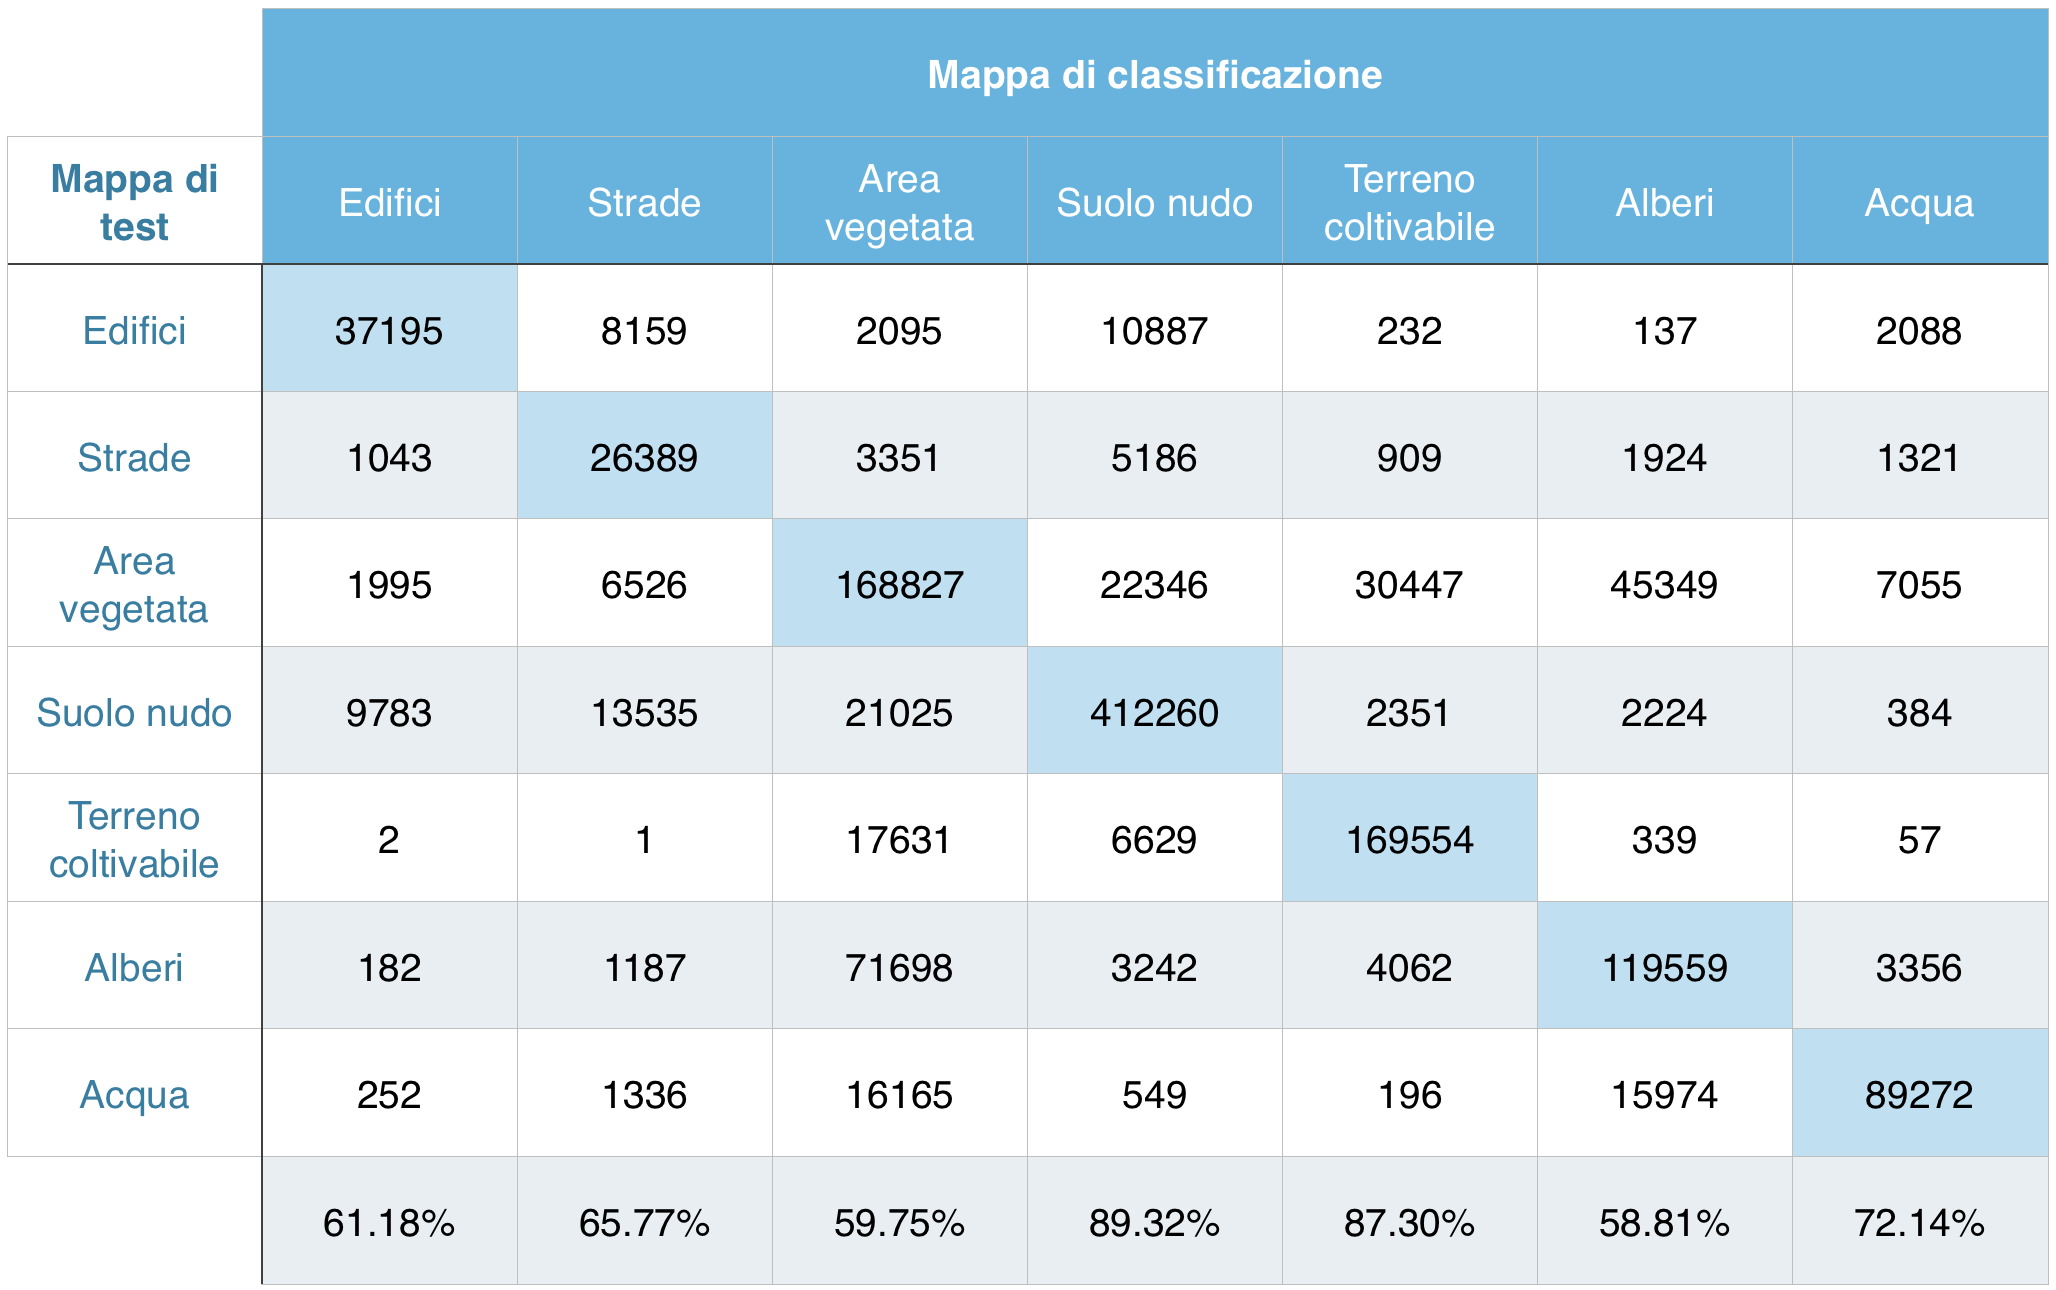
\includegraphics[width=1\textwidth]{Matrice_di_confusione_Amiens2006_2_5m_HOG_and_roads}
\caption{Mappa di classificazione del dataset \emph{Amiens 2006 - 2.5m - 7 classi}}
\label{fig:Matrice_di_confusione_Amiens2006_2_5m_HOG_and_roads}
\end{figure}


La particolarità di questo \emph{dataset} risiede nel fatto che, confrontando questi risultati con quelli senza estrazione di \emph{feature}, possono nascere dubbi sul reale beneficio di questo metodo di estrazione di 
\emph{feature} di tessitura. In Figura \ref{fig:Confronto_Amiens2006_2_5m_con_e_senza_hog_e_roads} vengono proposte le variazioni di prestazioni classe per classe.\\

\begin{figure}[!ht]
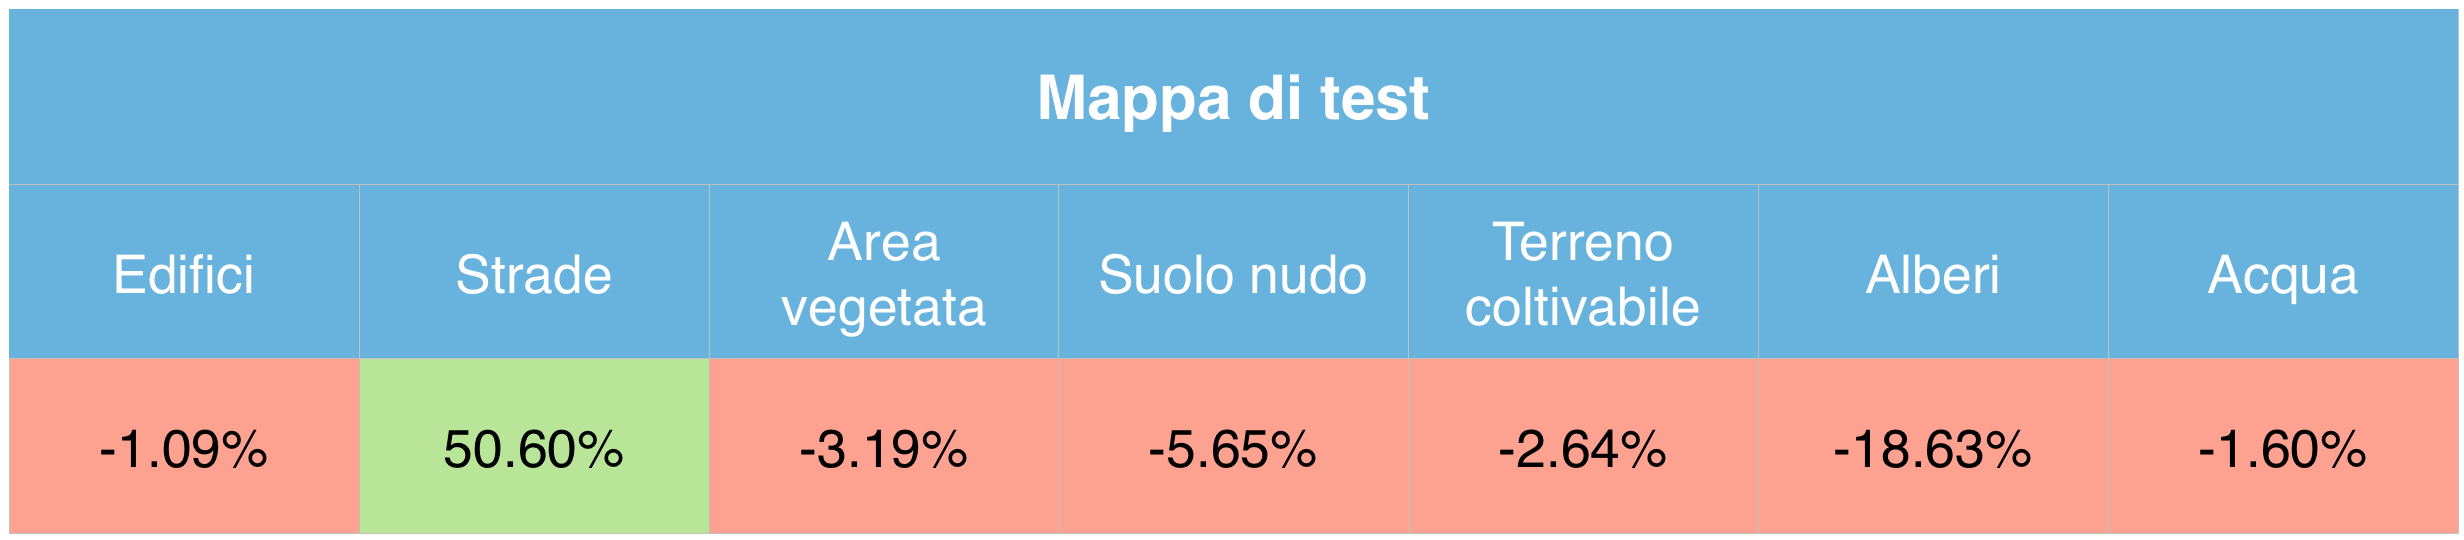
\includegraphics[width=1\textwidth]{Confronto_Amiens2006_2_5m_con_e_senza_hog_e_roads}
\caption{Confronto percentuale tra accuratezze classe per classe con e senza estrazione di \emph{feature} per il \emph{dataset} Amiens 2006 a $2.5$ m}
\label{fig:Confronto_Amiens2006_2_5m_con_e_senza_hog_e_roads}
\end{figure}

Si osserva chiaramente come l'introduzione delle \emph{feature} HOG peggiora (in alcuni casi anche drasticamente) quasi tutti i valori di precisione del classificatore.\\
Tuttavia, come era possibile ipotizzare già dopo l'analisi dei due precedenti esperimenti, l'uso di \emph{HOG}, unito all'aggiunta della mappa cartografica, permette di far registrare un incremento notevole alla classe deputata all'etichettatura delle strade, che senza HOG è sempre la classe che registra i livelli di accuratezza più bassi, spesso insufficienti a dare una buona rappresentazione della verità al suolo. 



%
%\chapter{Conclusioni}
% Si, possiamo dirci soddisfatti dei miglioramenti relativo. In particolare, è interessante che AA migliori sempre introducendo le feature HOG. In pratica, la differenza fra OA ed AA è che OA pesa gli errori commessi sulle varie classi in proporzione ai loro numeri di campioni di test, mentre AA li pesa in maniera uniforme. Quindi OA è influenzata maggiormente dagli errori sulle classi maggioritarie. Il fatto che AA migliori sempre con l'inclusione delle HOG suggerisce che queste feature aggiuntive permettano di discriminare meglio soprattutto classi minoritarie.
%Si tratta di accuratezze che, in assoluto, sono basse, ma la cosa è giustificata dalla difficoltà a discriminare classi così simili.

%% !TEX encoding = utf8
% !TEX root = ../main.tex


\chapter{CIao Title Here} % Main chapter title

\label{ChapterX} % Change X to a consecutive number; for referencing this chapter elsewhere, use \ref{ChapterX}


ciao ciao ciao ciao ciao ciao ciao ciao ciao ciao ciao ciao ciao ciao ciao ciao ciao ciao ciao ciao ciao ciao ciao ciao ciao ciao ciao ciao 
ciao ciao ciao ciao ciao ciao ciao ciao ciao ciao ciao ciao ciao ciao ciao ciao ciao ciao ciao ciao ciao ciao ciao ciao ciao ciao ciao ciao 
ciao ciao ciao ciao ciao ciao ciao ciao ciao ciao ciao ciao ciao ciao ciao ciao ciao ciao ciao ciao ciao ciao ciao ciao ciao ciao ciao ciao 
ciao ciao ciao ciao ciao ciao ciao ciao ciao ciao ciao ciao ciao ciao ciao ciao ciao ciao ciao ciao ciao ciao ciao ciao ciao ciao ciao ciao 
ciao ciao ciao ciao ciao ciao ciao ciao ciao ciao ciao ciao ciao ciao ciao ciao ciao ciao ciao ciao ciao ciao ciao ciao ciao ciao ciao ciao 
ciao ciao ciao ciao ciao ciao ciao ciao ciao ciao ciao ciao ciao ciao ciao ciao ciao ciao ciao ciao ciao ciao ciao ciao ciao ciao ciao ciao 
ciao ciao ciao ciao ciao ciao ciao ciao ciao ciao ciao ciao ciao ciao ciao ciao ciao ciao ciao ciao ciao ciao ciao ciao ciao ciao ciao ciao 
ciao ciao ciao ciao ciao ciao ciao ciao ciao ciao ciao ciao ciao ciao ciao ciao ciao ciao ciao ciao ciao ciao ciao ciao ciao ciao ciao ciao 
ciao ciao ciao ciao ciao ciao ciao ciao ciao ciao ciao ciao ciao ciao ciao ciao ciao ciao ciao ciao ciao ciao ciao ciao ciao ciao ciao ciao 
ciao ciao ciao ciao ciao ciao ciao ciao ciao ciao ciao ciao ciao ciao ciao ciao ciao ciao ciao ciao ciao ciao ciao ciao ciao ciao ciao ciao 
ciao ciao ciao ciao ciao ciao ciao ciao ciao ciao ciao ciao ciao ciao ciao ciao ciao ciao ciao ciao ciao ciao ciao ciao ciao ciao ciao ciao 
ciao ciao ciao ciao ciao ciao ciao ciao ciao ciao ciao ciao ciao ciao ciao ciao ciao ciao ciao ciao ciao ciao ciao ciao ciao ciao ciao ciao 
ciao ciao ciao ciao ciao ciao ciao ciao ciao ciao ciao ciao ciao ciao ciao ciao ciao ciao ciao ciao ciao ciao ciao ciao ciao ciao ciao ciao 
ciao ciao ciao ciao ciao ciao ciao ciao ciao ciao ciao ciao ciao ciao ciao ciao ciao ciao ciao ciao ciao ciao ciao ciao ciao ciao ciao ciao 
ciao ciao ciao ciao ciao ciao ciao ciao ciao ciao ciao ciao ciao ciao ciao ciao ciao ciao ciao ciao ciao ciao ciao ciao ciao ciao ciao ciao 
ciao ciao ciao ciao ciao ciao ciao ciao ciao ciao ciao ciao ciao ciao ciao ciao ciao ciao ciao ciao ciao ciao ciao ciao ciao ciao ciao ciao 
ciao ciao ciao ciao ciao ciao ciao ciao ciao ciao ciao ciao ciao ciao ciao ciao ciao ciao ciao ciao ciao ciao ciao ciao ciao ciao ciao ciao 
ciao ciao ciao ciao ciao ciao ciao ciao ciao ciao ciao ciao ciao ciao ciao ciao ciao ciao ciao ciao ciao ciao ciao ciao ciao ciao ciao ciao 
ciao ciao ciao ciao ciao ciao ciao ciao ciao ciao ciao ciao ciao ciao ciao ciao ciao ciao ciao ciao ciao ciao ciao ciao ciao ciao ciao ciao 
ciao ciao ciao ciao ciao ciao ciao ciao ciao ciao ciao ciao ciao ciao ciao ciao ciao ciao ciao ciao ciao ciao ciao ciao ciao ciao ciao ciao 
ciao ciao ciao ciao ciao ciao ciao ciao ciao ciao ciao ciao ciao ciao ciao ciao ciao ciao ciao ciao ciao ciao ciao ciao ciao ciao ciao ciao 
ciao ciao ciao ciao ciao ciao ciao ciao ciao ciao ciao ciao ciao ciao ciao ciao ciao ciao ciao ciao ciao ciao ciao ciao ciao ciao ciao ciao 
ciao ciao ciao ciao ciao ciao ciao ciao ciao ciao ciao ciao ciao ciao ciao ciao ciao ciao ciao ciao ciao ciao ciao ciao ciao ciao ciao ciao 
ciao ciao ciao ciao ciao ciao ciao ciao ciao ciao ciao ciao ciao ciao ciao ciao ciao ciao ciao ciao ciao ciao ciao ciao ciao ciao ciao ciao 



\label{Bibliography}

%\lhead{\emph{Bibliografia}} % Change the page header to say "Bibliography"

\bibliographystyle{acm} % Use the "unsrtnat" BibTeX style for formatting the Bibliography
\nocite{*}
\bibliography{Bibliography} % The references (bibliography) information are stored in the file named "Bibliography.bib"


\end{document}
